% ------------------------------------------------------------------------
% ------------------------------------------------------------------------
% Modelo UFSC para Trabalhos Academicos (tese de doutorado, dissertação de
% mestrado) utilizando a classe abntex2
%
% Autor: Alisson Lopes Furlani
% 	Modificações:
%	- 27/08/2019: Alisson L. Furlani, add 'glossaries' package
%   - 30/10/2019: Alisson L. Furlani, adjusted some spacing errors and changed math fonts
%   - 17/01/2020: Alisson L. Furlani, updated certification page
%   - 07/02/2020: Alisson L. Furlani, fixed table counter bug
%   - 11/03/2020: Alisson L. Furlani, changed greek letters in math and fixed citation style
%   - 14/09/2020: Alisson L. Furlani, little adjustments
%   - 30/08/2021: Alisson L. Furlani, add glossaries
% ------------------------------------------------------------------------
% ------------------------------------------------------------------------

\documentclass[
	% -- opções da classe memoir --
	12pt,				% tamanho da fonte
	%openright,			% capítulos começam em pág ímpar (insere página vazia caso preciso)
	oneside,			% para impressão no anverso. Oposto a twoside
	a4paper,			% tamanho do papel. 
	% -- opções da classe abntex2 --
	chapter=TITLE,		% títulos de capítulos convertidos em letras maiúsculas
	section=TITLE,		% títulos de seções convertidos em letras maiúsculas
	%subsection=TITLE,	% títulos de subseções convertidos em letras maiúsculas
	%subsubsection=TITLE,% títulos de subsubseções convertidos em letras maiúsculas
	% -- opções do pacote babel --
	english,			% idioma adicional para hifenização
	%french,				% idioma adicional para hifenização
	%spanish,			% idioma adicional para hifenização
	brazil				% o último idioma é o principal do documento
	]{abntex2}

\usepackage{setup/ufscthesisA4-alf}
\usepackage{float}
\usepackage{array,multirow,booktabs,ragged2e,tabularx}
\usepackage{xltabular}
\usepackage{xurl}
\usepackage{subcaption}

\addbibresource{aftertext/references.bib} % Seus arquivos de referências

% ajusta espaçamento das listas itemize e enumerate
\setitemize{topsep=0pt,itemsep=0pt,leftmargin=\parindent+\labelwidth-\labelsep}
\setenumerate{topsep=0pt,itemsep=0pt,leftmargin=\parindent+\labelwidth-\labelsep}

% define a macro \Autoref to allow multiple references to be passed to \autoref
\makeatletter
\newcommand\Autoref[1]{\@first@ref#1,@}
\def\@throw@dot#1.#2@{#1}% discard everything after the dot
\def\@set@refname#1{%    % set \@refname to autoefname+s using \getrefbykeydefault
	\edef\@tmp{\getrefbykeydefault{#1}{anchor}{}}%
	\xdef\@tmp{\expandafter\@throw@dot\@tmp.@}%
	\ltx@IfUndefined{\@tmp autorefnameplural}%
	{\def\@refname{\@nameuse{\@tmp autorefname}s}}%
	{\def\@refname{\@nameuse{\@tmp autorefnameplural}}}%
}
\def\@first@ref#1,#2{%
	\ifx#2@\autoref{#1}\let\@nextref\@gobble% only one ref, revert to normal \autoref
	\else%
	\@set@refname{#1}%  set \@refname to autoref name
	\@refname~\ref{#1}% add autoefname and first reference
	\let\@nextref\@next@ref% push processing to \@next@ref
	\fi%
	\@nextref#2%
}
\def\@next@ref#1,#2{%
	\ifx#2@ e~\ref{#1}\let\@nextref\@gobble% at end: print e+\ref and stop
	\else, \ref{#1}% print  ,+\ref and continue
	\fi%
	\@nextref#2%
}
\makeatother

% Cria comando para referenciar Anexo automaticamente \refanexo
\newcommand{\refanexo}[1]{\hyperref[#1]{Anexo~\ref{#1}}}

% Define comandos para tabelas que permite ajustar o tamanho da coluna e manter alinhamento C, R ou L
%\newcommand{\PreserveBackslash}[1]{\let\temp=\\#1\let\\=\temp}
\newcolumntype{C}[1]{>{\centering\let\arraybackslash}m{#1}}
\newcolumntype{R}[1]{>{\RaggedLeft\let\arraybackslash}m{#1}}
\newcolumntype{L}[1]{>{\RaggedRight\let\arraybackslash}m{#1}}

% ---
% Filtering and Mapping Bibliographies
% ---
\DeclareSourcemap{
	\maps[datatype=bibtex]{
		% remove fields that are always useless
		\map{
			\step[fieldset=abstract, null]
			\step[fieldset=pagetotal, null]
			\step[fieldset=doi, null]
		}
		% remove URLs for types that are primarily printed
		\map{
			\pernottype{software}
			\pernottype{online}
			\pernottype{report}
			\pernottype{techreport}
			\pernottype{standard}
			\pernottype{manual}
			\pernottype{misc}
			\step[fieldset=url, null]
			\step[fieldset=urldate, null]
		}
		\map{
			\pertype{inproceedings}
			% remove mostly redundant conference information
			%\step[fieldset=venue, null]
			%\step[fieldset=eventdate, null]
			%\step[fieldset=eventtitle, null]
			% do not show ISBN for proceedings
			\step[fieldset=isbn, null]
			% Citavi bug
			%\step[fieldset=volume, null]
		}
	}
}
% ---

% ---
% Informações de dados para CAPA e FOLHA DE ROSTO
% ---
% FIXME Substituir 'Nome completo do autor' pelo seu nome.
\autor{Gabriel de Oliveira Aguiar}
% FIXME Substituir 'Título do trabalho' pelo título da trabalho.
\titulo{Crash-Aware Traffic Prioritization in Vehicular Wi-Fi Networks}
% FIXME Substituir 'Subtítulo (se houver)' pelo subtítulo da trabalho.  
% Caso não tenha substítulo, comente a linha a seguir.
% \subtitulo{Uma Alternativa de Baixo Custo}
% FIXME Substituir 'XXXXXX' pelo nome do seu
% orientador.
\orientador[Supervisor]{Prof. Giovani Gracioli, Ph.D.}
% FIXME Se for orientado por uma mulher, comente a linha acima e descomente a linha a seguir.
% \orientador[Supervisor]{Nome da orientadora, Dra.}
% FIXME Substituir 'XXXXXX' pelo nome do seu
% coorientador. Caso não tenha coorientador, comente a linha a seguir.
% \coorientador{Prof. XXXXXX, Dr.}
% FIXME Se for coorientado por uma mulher, comente a linha acima e descomente a linha a seguir.
% \coorientador[Co-supervisor]{XXXXXX, Dra.}
% FIXME Substituir '[ano]' pelo ano (ano) em que seu trabalho foi defendido.
\ano{2026}
% FIXME Substituir '[dia] de [mês] de [ano]' pela data em que ocorreu sua defesa.
%\data{[dia] de [mês] de [ano]}
% FIXME Substituir 'Local' pela cidade em que ocorreu sua defesa.
\local{Florianópolis}
\instituicaosigla{UFSC}
\instituicao{Universidade Federal de Santa Catarina}
% FIXME Substituir 'Dissertação/Tese' pelo tipo de trabalho (Tese, Dissertação). 
\tipotrabalho{Master's Dissertation}
% FIXME Substituir '[mestre/doutor] em XXXXXX' pela grau adequado.
\formacao{Master of Science in Computer Science}
% FIXME Substituir '[mestrado/doutorado]' pelo nivel adequado.
\nivel{Master's}
% FIXME Substituir 'Programa de Pós-Graduação em XXXXXX' pela curso adequado.
\programa{Graduate Program in Computer Science}
% FIXME Substituir 'Campus XXXXXX ou Centro de XXXXXX' pelo campus ou centro adequado.
\centro{Campus Reitor João David Ferreira Lima}
\preambulo
{%
\imprimirtipotrabalho~submitted~to~the~\imprimirprograma~of~the~\imprimirinstituicao~as~a~requirement~for~obtaining~the~degree~of~\imprimirformacao.
}
% ---

% ---
% Configurações de aparência do PDF final
% ---
% alterando o aspecto da cor azul
\definecolor{blue}{RGB}{41,5,195}
% informações do PDF
\makeatletter
\hypersetup{
     	%pagebackref=true,
		pdftitle={\@title}, 
		pdfauthor={\@author},
    	pdfsubject={\imprimirpreambulo},
	    pdfcreator={LaTeX with abnTeX2},
		pdfkeywords={ufsc, v2x, vehicular networks, ieee 802.11p, qos, edca, crash-aware}, 
		colorlinks=true,       		% false: boxed links; true: colored links
    	linkcolor=black,%blue,          	% color of internal links
    	citecolor=black,%blue,        		% color of links to bibliography
    	filecolor=black,%magenta,      		% color of file links
		urlcolor=black,%blue,
		breaklinks=true,       		% allow line breaks inside citation/hyperref links
		bookmarksdepth=4
}
\makeatother

% Allow ABNT author-year citations to break after ; and , so they stay inside margins
\DeclareDelimFormat{multinamedelim}{\addsemicolon\allowbreak\space}
\DeclareDelimFormat{finalnamedelim}{\addsemicolon\allowbreak\space}
\DeclareDelimFormat{nameyeardelim}{\addcomma\allowbreak\space}
\DeclareDelimFormat{andothersdelim}{\addcomma\allowbreak\space}
\setlength{\emergencystretch}{3em}
% ---

% ---
% Lista de abreviaturas e siglas / símbolos
% Descrição em inglês (expansão no texto); user1 em português (lista bilíngue)
% Only entries used via \gls/\glspl appear in the printed list.
% ---

\newacronym[user1=\emph{Projeto de Parceria de 3ª Geração}]{threegpp}{3GPP}{3rd Generation Partnership Project}
\newacronym[user1=\emph{categoria de acesso}]{ac}{AC}{Access Category}
\newacronym[user1=\emph{confirmação de recebimento}]{ack}{ACK}{Acknowledgment}
\newacronym[user1=\emph{espaço entre quadros de arbitragem}]{aifs}{AIFS}{Arbitration Interframe Space}
\newacronym[user1=\emph{número do espaço entre quadros de arbitragem}]{aifsn}{AIFSN}{Arbitration Interframe Space Number}
\newacronym[user1=\emph{melhor esforço}]{be}{BE}{Best Effort}
\newacronym[user1=\emph{retirada exponencial binária}]{beb}{BEB}{Binary Exponential Backoff}
\newacronym[user1=\emph{categoria background}]{bk}{BK}{Background}
\newacronym[user1=\emph{mensagem básica de segurança}]{bsm}{BSM}{Basic Safety Message}
\newacronym[user1=\emph{conjunto básico de serviços}]{bss}{BSS}{Basic Service Set}
\newacronym[user1=\emph{mensagem de consciência cooperativa}]{cam}{CAM}{Cooperative Awareness Message}
\newacronym[user1=\emph{razão de ocupação do canal}]{cbr}{CBR}{Channel Busy Ratio}
\newacronym[user1=\emph{canal de controle}]{cch}{CCH}{Control Channel}
\newacronym[user1=\emph{acesso múltiplo por detecção de portadora com prevenção de colisões}]{csma}{CSMA/CA}{Carrier Sense Multiple Access with Collision Avoidance}
\newacronym[user1=\emph{autorização para enviar}]{cts}{CTS}{Clear to Send}
\newacronym[user1=\emph{janela de contenção}]{cw}{CW}{Contention Window}
\newacronym[user1=\emph{controle de congestionamento descentralizado}]{dcc}{DCC}{Decentralized Congestion Control}
\newacronym[user1=\emph{função de coordenação distribuída}]{dcf}{DCF}{Distributed Coordination Function}
\newacronym[user1=\emph{mensagem de notificação ambiental descentralizada}]{denm}{DENM}{Decentralized Environmental Notification Message}
\newacronym[user1=\emph{espaço entre quadros DCF}]{difs}{DIFS}{DCF Interframe Space}
\newacronym[user1=\emph{serviços diferenciados}]{diffserv}{DiffServ}{Differentiated Services}
\newacronym[user1=\emph{ponto de código de serviços diferenciados}]{dscp}{DSCP}{Differentiated Services Code Point}
\newacronym[user1=\emph{comunicações dedicadas de curto alcance}]{dsrc}{DSRC}{Dedicated Short-Range Communications}
\newacronym[user1=\emph{acesso ao canal distribuído aprimorado}]{edca}{EDCA}{Enhanced Distributed Channel Access}
\newacronym[user1=\emph{função de coordenação distribuída aprimorada}]{edcf}{EDCF}{Enhanced Distributed Coordination Function}
\newacronym[user1=\emph{encaminhamento acelerado}]{ef}{EF}{Expedited Forwarding}
\newacronym[user1=\emph{Instituto Europeu de Normas de Telecomunicações}]{etsi}{ETSI}{European Telecommunications Standards Institute}
\newacronym[user1=\emph{máquina de estados finitos}]{fsm}{FSM}{Finite-State Machine}
\newacronym[user1=\emph{retransmissão de grupo confiável}]{gcr}{GCR}{Groupcast with Retries}
\newacronym[user1=\emph{função de coordenação híbrida}]{hcf}{HCF}{Hybrid Coordination Function}
\newacronym[user1=\emph{acesso ao canal controlado por HCF}]{hcca}{HCCA}{HCF Controlled Channel Access}
\newacronym[user1=\emph{instituto de engenheiros eletricistas e eletrônicos}]{ieee}{IEEE}{Institute of Electrical and Electronics Engineers}
\newacronym[user1=\emph{framework de redes do OMNeT++}]{inet}{INET}{INET Framework}
\newacronym[user1=\emph{protocolo de internet}]{ip}{IP}{Internet Protocol}
\newacronym[user1=\emph{protocolo de internet versão 4}]{ipv4}{IPv4}{Internet Protocol version 4}
\newacronym[user1=\emph{protocolo de internet versão 6}]{ipv6}{IPv6}{Internet Protocol version 6}
\newacronym[user1=\emph{sistemas inteligentes de transporte}]{its}{ITS}{Intelligent Transportation Systems}
\newacronym[user1=\emph{comunicação entre veículos}]{ivc}{IVC}{Inter-Vehicle Communication}
\newacronym[user1=\emph{indicador-chave de desempenho}]{kpi}{KPI}{Key Performance Indicator}
\newacronym[user1=\emph{controle de acesso ao meio}]{mac}{MAC}{Medium Access Control}
\newacronym[user1=\emph{unidade de dados de serviço MAC}]{msdu}{MSDU}{MAC Service Data Unit}
\newacronym[user1=\emph{descrição de rede do OMNeT++}]{ned}{NED}{Network Description}
\newacronym[user1=\emph{fora do contexto de um BSS}]{ocb}{OCB}{Outside the Context of a BSS}
\newacronym[user1=\emph{multiplexação ortogonal por divisão de frequência}]{ofdm}{OFDM}{Orthogonal Frequency-Division Multiplexing}
\newacronym[user1=\emph{acesso múltiplo por divisão de frequência ortogonal}]{ofdma}{OFDMA}{Orthogonal Frequency-Division Multiple Access}
\newacronym[user1=\emph{simulador de redes de eventos discretos}]{omnet}{OMNeT++}{Objective Modular Network Testbed in C++}
\newacronym[user1=\emph{percentil 95}]{p95}{P95}{95th percentile}
\newacronym[user1=\emph{comportamento por salto}]{phb}{PHB}{Per-Hop Behavior}
\newacronym[user1=\emph{camada física}]{phy}{PHY}{Physical Layer}
\newacronym[user1=\emph{qualidade de serviço}]{qos}{QoS}{Quality of Service}
\newacronym[user1=\emph{pedido de comentários}]{rfc}{RFC}{Request for Comments}
\newacronym[user1=\emph{unidade de beira de estrada}]{rsu}{RSU}{Roadside Unit}
\newacronym[user1=\emph{solicitação para enviar}]{rts}{RTS}{Request to Send}
\newacronym[user1=\emph{canal de serviço}]{sch}{SCH}{Service Channel}
\newacronym[user1=\emph{espaço entre quadros curto}]{sifs}{SIFS}{Short Interframe Space}
\newacronym[user1=\emph{relação sinal-ruído-mais-interferência}]{snir}{SNIR}{Signal-to-Noise-plus-Interference Ratio}
\newacronym[user1=\emph{agendamento semi-persistente}]{sps}{SPS}{Semi-Persistent Scheduling}
\newacronym[user1=\emph{simulação de mobilidade urbana}]{sumo}{SUMO}{Simulation of Urban MObility}
\newacronym[user1=\emph{modelador ciente do tempo}]{tas}{TAS}{Time-Aware Shaper}
\newacronym[user1=\emph{acesso múltiplo por divisão de tempo}]{tdma}{TDMA}{Time Division Multiple Access}
\newacronym[user1=\emph{controle de potência de transmissão}]{tpc}{TPC}{Transmit Power Control}
\newacronym[user1=\emph{interface de controle de tráfego}]{traci}{TraCI}{Traffic Control Interface}
\newacronym[user1=\emph{controle de taxa de transmissão}]{trc}{TRC}{Transmit Rate Control}
\newacronym[user1=\emph{redes sensíveis ao tempo}]{tsn}{TSN}{Time-Sensitive Networking}
\newacronym[user1=\emph{oportunidade de transmissão}]{txop}{TXOP}{Transmission Opportunity}
\newacronym[user1=\emph{veículo aéreo não tripulado}]{uav}{UAV}{Unmanned Aerial Vehicle}
\newacronym[user1=\emph{protocolo de datagrama do usuário}]{udp}{UDP}{User Datagram Protocol}
\newacronym[user1=\emph{prioridade de usuário}]{up}{UP}{User Priority}
\newacronym[user1=\emph{comunicação ultraconfiável de baixa latência}]{urllc}{URLLC}{Ultra-Reliable Low-Latency Communication}
\newacronym[user1=\emph{comunicação veículo-a-tudo}]{v2x}{V2X}{Vehicle-to-Everything}
\newacronym[user1=\emph{comunicação veículo-a-veículo}]{v2v}{V2V}{Vehicle-to-Vehicle}
\newacronym[user1=\emph{rede ad hoc veicular}]{vanet}{VANET}{Vehicular Ad hoc Network}
\newacronym[user1=\emph{framework de simulação veicular}]{veins}{Veins}{Vehicles in Network Simulation}
\newacronym[user1=\emph{voz}]{vo}{VO}{Voice}
\newacronym[user1=\emph{vídeo}]{vi}{VI}{Video}
\newacronym[user1=\emph{acesso sem fio em ambientes veiculares}]{wave}{WAVE}{Wireless Access in Vehicular Environments}

% Declaração dos símbolos (usados no texto/equações; lista ordenada por primeira ocorrência)
\simbololista{cwmin}{\ensuremath{\mathrm{CW}_{\min}}}{Minimum contention window}
\simbololista{cwmax}{\ensuremath{\mathrm{CW}_{\max}}}{Maximum contention window}
\simbololista{W}{\ensuremath{W}}{Current contention-window size}
\simbololista{pcol}{\ensuremath{p}}{Conditional collision probability}
\simbololista{tau}{\ensuremath{\tau}}{Per-slot transmission probability}
\simbololista{mback}{\ensuremath{m}}{Maximum backoff stage}
\simbololista{aifs_i}{\ensuremath{\mathrm{AIFS}[i]}}{Arbitration interframe space of access category $i$}
\simbololista{aifsn_i}{\ensuremath{\mathrm{AIFSN}[i]}}{AIFSN parameter of access category $i$}
\simbololista{sifs_sym}{\ensuremath{\mathrm{SIFS}}}{Short interframe space duration}
\simbololista{slot}{\ensuremath{a\mathrm{SlotTime}}}{Slot time}


% compila a lista de abreviaturas e siglas e a lista de símbolos
\makenoidxglossaries 

% ---

% ---
% compila o indice
% ---
\makeindex
% ---
% \usepackage[inline]{enumitem} % no preâmbulo
% \usepackage{paralist}
\usepackage{siunitx}
\usepackage{amsmath}
\usepackage{adjustbox}

\newcommand{\E}{\mathbb{E}}
\newcommand{\Var}{\operatorname{Var}}

\usepackage{todonotes}

\pdfminorversion=7
\pdfobjcompresslevel=3
\pdfcompresslevel=2


% ----
% Início do documento
% ----
\begin{document}

% Seleciona o idioma do documento (conforme pacotes do babel)
\selectlanguage{english}
% \selectlanguage{brazil}

% Retira espaço extra obsoleto entre as frases.
\frenchspacing 

% Espaçamento 1.5 entre linhas
\OnehalfSpacing

% Corrige justificação
%\sloppy

% ----------------------------------------------------------
% ELEMENTOS PRÉ-TEXTUAIS
% ----------------------------------------------------------
% \pretextual %a macro \pretextual é acionado automaticamente no início de \begin{document}
% ---
% Capa, folha de rosto, ficha bibliografica, errata, folha de apróvação
% Dedicatória, agradecimentos, epígrafe, resumos, listas
% ---
% ---
% Capa
% ---
\imprimircapa
% ---

% ---
% Folha de rosto
% (o * indica que haverá a ficha bibliográfica)
% ---
\imprimirfolhaderosto*
% ---

% ---
% Inserir a ficha bibliografica
% ---
% http://ficha.bu.ufsc.br/
% \begin{fichacatalografica}
% 	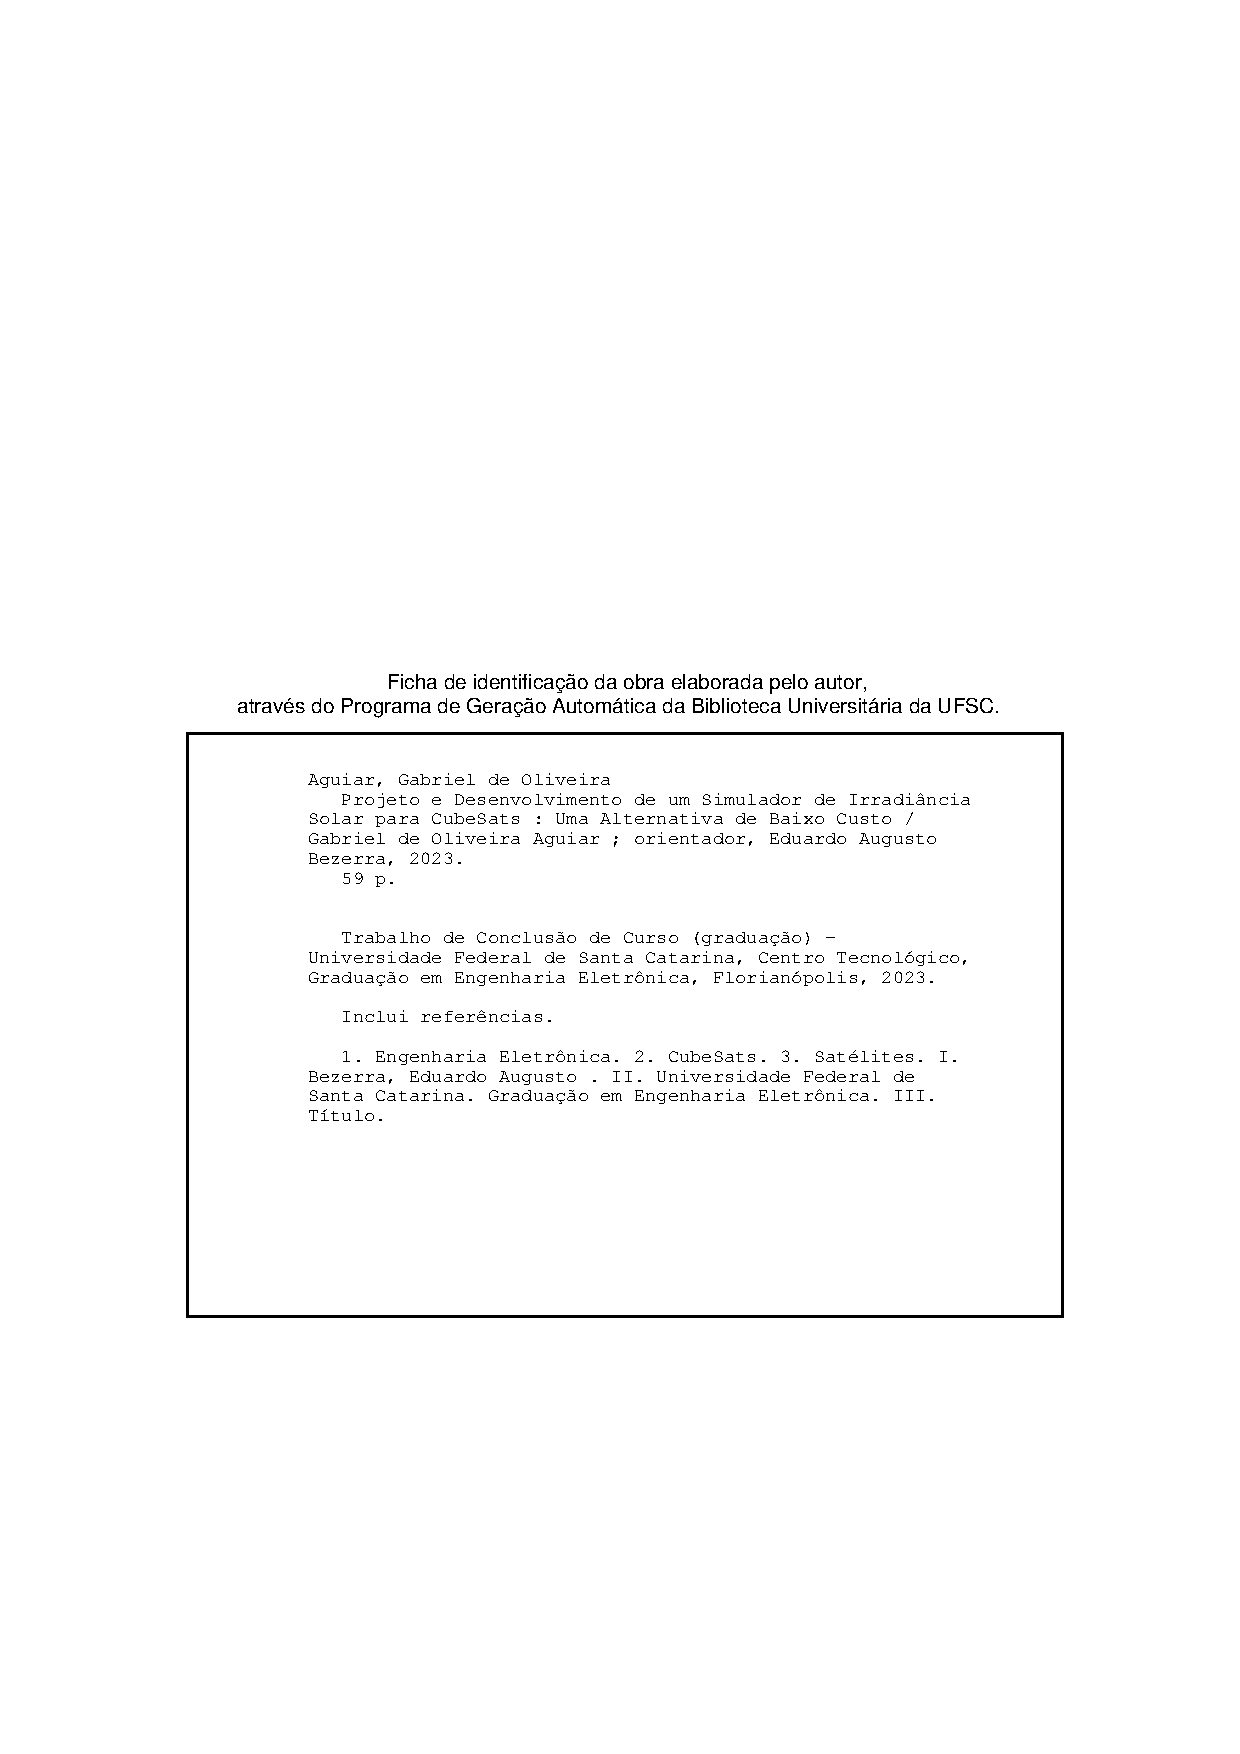
\includepdf{beforetext/Ficha_Catalografica.pdf}
% \end{fichacatalografica}
% ---

% ---
% Inserir folha de aprovação
% ---
% \begin{folhadeaprovacao}
% 	\OnehalfSpacing
% 	\centering
% 	\imprimirautor\\%
% 	\vspace*{10pt}		
% 	\textbf{\imprimirtitulo}%
% 	\ifnotempty{\imprimirsubtitulo}{:~\imprimirsubtitulo}\\%
% 	\vspace*{\baselineskip}
% 	This Master's Thesis was deemed suitable for the attainment of the Master of Science in Computer Science and was approved in its final form by the Graduate Program in Computer Science of INE - Department Of Informatics and Statistics, CTC - Technological Center of Universidade Federal de Santa Catarina.\\
%     \vspace*{\baselineskip}
%     Florianópolis, July 14, 2025. \\
% 	\vspace*{\baselineskip}
%  	\assinatura{\OnehalfSpacing Prof. xxxxxxx, Ph.D. \\ Graduate Program Coordinator}

%  	\vspace*{\baselineskip}
% 	\textbf{Examination Committee}\\
% 	\assinatura{\OnehalfSpacing\imprimirorientador \\ \imprimirorientadorRotulo}
% 	\vspace*{\fill}
%  	\assinatura{\OnehalfSpacing xxxxxxx, Eng.\\
% 	Federal University of Santa Catarina}
% 	\vspace*{\fill}
%  	\assinatura{\OnehalfSpacing xxxxxxx, M.Sc.\\
% 	Federal University of Santa Catarina\\}
% 	\vspace*{\fill}
% 	\assinatura{Prof. xxxxxxx, Ph.D.\\
% 	Federal University of Santa Catarina}

% 	\vspace*{\fill}
% 	\imprimirlocal, \imprimirano.
% \end{folhadeaprovacao}

% ---

% ---
% Dedicatória
% ---
% \begin{dedicatoria}
% 	\vspace*{\fill}
% 	\noindent
% 	\begin{adjustwidth*}{}{5.5cm} 
% 		\raggedleft       
% 		Sou grato aos meus amigos e familiares, que me apoiaram emocionalmente ao longo desta jornada acadêmica.
% 	\end{adjustwidth*}
% \end{dedicatoria}
% ---

% ---
% Agradecimentos
% ---
% \begin{agradecimentos}
% Aos meus amados pais, Leila Rosa de Oliveira e Antonio Neto Aguiar, que sempre estiveram ao meu lado, me apoiando incondicionalmente e estimulando minha busca pelo conhecimento.

% Ao meu dedicado orientador, Eduardo Bezerra, pelo seu valioso suporte, paciência e dedicação ao longo deste trabalho, além de disponibilizar o espaço no SPACELAB, que foi fundamental para a realização deste artigo.

% Agradeço de coração ao grupo AZCD, do qual faço parte e considero uma verdadeira família, pelo apoio inestimável. Sem eles, eu não seria quem sou hoje.

% Aos meus colegas do SPACELAB, em especial a João Cláudio Elsen Barcellos, pelo apoio direto no projeto e por incentivarem minhas ideias com entusiasmo.

% E, por fim, gostaria de expressar minha gratidão à Carolina Bassi, minha leal namorada e parceira, por seu apoio constante ao longo dessa jornada acadêmica.
% \end{agradecimentos}
% ---

% ---
% Epígrafe
% ---
% \begin{epigrafe}
% 	\vspace*{\fill}
% 	\begin{flushright}
% 		\textit{``The ideal engineer is a composite... \\ He is not a scientist, he is not a mathematician, \\he is not a sociologist or a writer;\\ but he may use the knowledge and techniques \\ of any or all of these disciplines in solving engineering problems.''\\
% 			(Dougherty, 1955)}
% 	\end{flushright}
% \end{epigrafe}
% ---

% ---
% RESUMOS
% ---

% resumo em português

\setlength{\absparsep}{18pt} % ajusta o espaçamento dos parágrafos do resumo
\begin{resumo}[Resumo]
	\SingleSpacing
	Alertas de colisão em comunicação veículo-a-tudo (\emph{Vehicle-to-Everything}, V2X) são mensagens raras, porém de alto impacto, cuja utilidade depende de entrega oportuna sob contenção de canal. Em redes IEEE 802.11p descentralizadas, esses alertas compartilham o meio com o tráfego de rotina, de modo que picos de atraso e congelamento de \emph{backoff} podem corroer sua prioridade sob carga. Esta dissertação avalia uma estratégia focada de priorização ciente de colisão na qual todos os veículos trocam tráfego \emph{multicast} periódico de melhor esforço (\emph{Best Effort}, BE), enquanto um veículo acidentado emite rajadas temporárias de alerta marcadas com \emph{Differentiated Services Code Point} (DSCP) 46 e mapeadas para a categoria de voz (\emph{Voice}, VO). Usando OMNeT++, Veins e INET, cinco políticas de controle de acesso ao meio (MAC) são comparadas em cenários de rodovia com 10 e 100 veículos: uma linha de base com \emph{Distributed Coordination Function} (DCF), \emph{Enhanced Distributed Channel Access} (EDCA) com mapeamento explícito de DSCP para voz, e três extensões adaptativas que temporariamente adiam ou descartam o tráfego BE concorrente enquanto os alertas estão ativos, todas sem exigir mudanças de protocolo ou infraestrutura. Sob congestionamento intenso, a preempção de emergência reduz o atraso de percentil 95 dos alertas de colisão em cerca de 49\% em relação ao EDCA (de 0,90 ms para 0,46 ms), ao custo de maior atraso BE e perdas BE explícitas; sob contenção leve, a supressão limitada penaliza principalmente o BE sem melhorar os alertas. Os resultados caracterizam uma fronteira proteção-custo e indicam que o bloqueio adaptativo deve ser uma escalada acionada por eventos, e não um modo de QoS permanentemente ativo.

	\textbf{Palavras-chave}: V2X. Wi-Fi Veicular. IEEE 802.11p. EDCA. Qualidade de Serviço. Priorização Ciente de Colisão.
\end{resumo}

% resumo em inglês
\begin{resumo}[Abstract]
	\SingleSpacing
	\begin{otherlanguage*}{english}
	Vehicle-to-everything (V2X) crash alerts are rare but high-impact messages whose usefulness depends on timely delivery under channel contention. In decentralized IEEE 802.11p networks they share the medium with routine traffic, so delay spikes and backoff freezing can erode their priority under load. This dissertation evaluates a focused crash-aware prioritization strategy in which all vehicles exchange periodic Best Effort (BE) multicast traffic while one crash vehicle emits temporary alert bursts marked with Differentiated Services Code Point (DSCP) 46 and mapped to Voice (VO). Using OMNeT++, Veins, and INET, five Medium Access Control (MAC) policies are compared on highway scenarios with 10 and 100 vehicles: a Distributed Coordination Function (DCF) baseline, Enhanced Distributed Channel Access (EDCA) with explicit DSCP-to-Voice mapping, and three adaptive extensions that temporarily suppress or drop competing BE traffic while alerts are active, all requiring no protocol changes or infrastructure. Under heavy congestion, emergency preemption reduces crash-alert 95th-percentile delay by about 49\% relative to EDCA (from 0.90 ms to 0.46 ms), at the cost of higher BE delay and explicit BE losses; under light contention, bounded suppression mainly penalizes BE without improving alerts. The results characterize a protection-versus-cost frontier and indicate that adaptive blocking should be an event-triggered escalation rather than an always-on QoS mode.

		\textbf{Keywords}: V2X. Vehicular Wi-Fi. IEEE 802.11p. EDCA. Quality of Service. Crash-Aware Prioritization.
	\end{otherlanguage*}
\end{resumo}

%% resumo em francês 
%\begin{resumo}[Résumé]
% \begin{otherlanguage*}{french}
%    Il s'agit d'un résumé en français.
% 
%   \textbf{Mots-clés}: latex. abntex. publication de textes.
% \end{otherlanguage*}
%\end{resumo}
%
%% resumo em espanhol
%\begin{resumo}[Resumen]
% \begin{otherlanguage*}{spanish}
%   Este es el resumen en español.
%  
%   \textbf{Palabras clave}: latex. abntex. publicación de textos.
% \end{otherlanguage*}
%\end{resumo}
%% ---

{%hidelinks
	\hypersetup{hidelinks}
	% ---
	% inserir lista de ilustrações
	% ---
	\pdfbookmark[0]{\listfigurename}{lof}
	\listoffigures*
	\cleardoublepage
	% ---
	
	% ---
	% inserir lista de quadros
	% ---
	% \pdfbookmark[0]{\listofquadrosname}{loq}
	% \listofquadros*
	% \cleardoublepage
	% ---
	
	% ---
	% inserir lista de tabelas
	% ---
	\pdfbookmark[0]{\listtablename}{lot}
	\listoftables*
	\cleardoublepage
	% ---
	
	% ---
	% inserir lista de abreviaturas e siglas (devem ser declarados no preambulo)
	% ---
	% \imprimirlistadesiglas
	% ---
	
	% ---
	% inserir lista de símbolos (devem ser declarados no preambulo)
	% ---
	% \imprimirlistadesimbolos
	% ---
	
	% ---
	% inserir o sumario
	% ---
	\pdfbookmark[0]{\contentsname}{toc}
	\tableofcontents*
	\cleardoublepage
	
}%hidelinks
% ---
% ---

% ----------------------------------------------------------
% ELEMENTOS TEXTUAIS
% ----------------------------------------------------------
\textual

% ---
% 0 - Introdução
% ---
\chapter{Introduction}
\label{chap:intro}

Cooperative vehicular applications depend on the timely wireless dissemination of safety-relevant information among nearby vehicles. \gls{v2x} communication enables vehicles to exchange messages directly with other vehicles, infrastructure, and pedestrians, and \gls{ieee}~802.11 remains an important reference technology for this purpose because it supports direct, decentralized exchanges without continuous infrastructure support \cite{IEEE_80211p_Survey}. In particular, IEEE~802.11p adapts the standard for vehicular operation, typically at 5.9~GHz with 10~MHz channelization, and relies on fully distributed channel access: there is no central scheduler that can reserve transmission opportunities for urgent traffic.

Among the messages exchanged in such networks, crash alerts occupy a special position. They are rare, but when they occur, their usefulness depends almost entirely on timely delivery to nearby vehicles. Contention-based channel access, however, exposes this urgent crash-related traffic to the same medium competition faced by routine transmissions: as offered load rises, delay and jitter become unstable, backoff freezing can postpone emergency frames while the channel is busy, and \gls{qos} markings are not handled consistently across deployments \cite{RFC8325_WiFi_QoS, Continuous_Backoff_Freezing_Li}. A crash alert that arrives late competes for the channel exactly when the surrounding traffic is most likely to be dense, which is also when its delivery matters most.

Within IEEE~802.11, two standard mechanisms are central to traffic differentiation. At the network layer, \gls{dscp} marking expresses traffic criticality; at the link layer, \gls{edca} translates that criticality into differentiated medium access through access categories with distinct contention parameters \cite{IEEE80211}. The resulting wireless behavior, however, depends on the local policy that maps DSCP values into 802.11 user priorities and then into EDCA queues, and default mappings are ambiguous in practice \cite{RFC8325_WiFi_QoS}. Moreover, EDCA provides statistical preference rather than guarantees: higher-priority categories obtain access earlier on average, but all categories still contend randomly, and urgent traffic improves only at the expense of lower-priority flows.

Recent literature pursues stronger contention control through slot-based schedulers inspired by \gls{tsn}, preemptive or cooperative \gls{mac} schemes, and cellular sidelink resource allocation \cite{TSNCtl_Feraudo, PRP_MAC_Li, CFC_MAC_Linn, CV2X_Sidelink_Allocation}. These approaches confirm the value of tighter contention control, but they rely on synchronization, infrastructure, or richer protocol machinery, assumptions that are difficult to satisfy in a decentralized vehicular ad hoc network. This leaves a practical gap for a local, event-driven design that isolates one crash-triggered high-priority flow against ordinary background traffic and quantifies both the protection obtained and the penalty imposed. Staying within standard IEEE~802.11p mechanisms keeps such a design deployable: no clock synchronization, infrastructure, or protocol changes are required, and adoption can proceed per node.

This dissertation addresses that gap with a deliberately narrow study: a focused crash-aware prioritization strategy built from standard mechanisms rather than a new MAC protocol. All vehicles exchange periodic \gls{be} multicast traffic, while one designated crash vehicle emits temporary alert bursts marked with DSCP~46 and mapped to the \gls{vo} access category. On top of this two-class model, five MAC policies are compared: a plain \gls{dcf} baseline, EDCA with explicit DSCP-to-Voice mapping, and three adaptive extensions (\texttt{stable}, \texttt{guarded}, and \texttt{emergency}) that temporarily suppress or drop competing BE traffic while alerts are active. The adaptive profiles are fixed design points that map a protection-versus-cost frontier, aiming at better statistical latency under congestion rather than deterministic guarantees.

\section{Research Question and Scope}
\label{sec:intro:question}

The central question investigated in this dissertation is:

\begin{quote}
	Can crash-triggered traffic obtain better wireless service than ordinary traffic in Veins/\gls{inet} simulations, and what cost does that protection impose on ordinary traffic?
\end{quote}

The scope is intentionally minimal. The study considers a single crash source, a two-class BE/VO traffic distinction, and one-hop multicast dissemination on a highway corridor, with no access points, roadside units, or centralized coordination. It does not attempt to reproduce a full \gls{its} stack, standardized cooperative-awareness message schedules, or multi-class traffic orchestration. All findings are obtained by simulation in \gls{omnet}/Veins/\gls{inet}, and all observed prioritization is statistical contention shaping: no deterministic slotting, synchronization, or provable worst-case bounds are claimed.

\section{Objectives}
\label{sec:intro:objectives}

The general objective of this dissertation is to evaluate, through simulation, whether crash-triggered Voice traffic can obtain measurably better wireless service than ordinary Best Effort traffic in decentralized vehicular Wi-Fi, using only local, standard-compliant MAC mechanisms, and to quantify the cost that this protection imposes on ordinary traffic.

The specific objectives are:

\begin{enumerate}
	\item To implement a crash-triggered two-class traffic model in Veins/\gls{inet}, in which all vehicles generate periodic BE multicast traffic and a designated crash vehicle emits DSCP~46 alert bursts mapped to the VO access category through an explicit classifier.
	\item To design and implement a lightweight adaptive MAC controller that extends EDCA with a local three-mode protection mechanism, exposed as a ladder of five policies with increasing aggressiveness, from plain DCF to emergency preemption.
	\item To evaluate the five policies across a matrix of vehicle densities (10 and 100 vehicles) and offered-load profiles, using class-specific delay, jitter, multicast reach, and MAC-loss metrics.
	\item To characterize the resulting protection-versus-cost frontier and derive engineering guidance on when adaptive suppression should be enabled.
\end{enumerate}

\section{Contributions}
\label{sec:intro:contributions}

This dissertation makes the following primary contributions:

\begin{enumerate}
	\item A lightweight adaptive MAC controller built solely from standard mechanisms---explicit DSCP~46-to-Voice mapping plus a local three-mode extension of EDCA---applied to a crash-triggered two-class traffic model in which ordinary vehicular multicast traffic remains Best Effort while a designated crash node injects temporary Voice alert bursts.
	\item An open-source Veins/\gls{inet} simulation artifact \cite{aguiar2026_veins_qos} comparing a plain IEEE~802.11p DCF baseline, an EDCA baseline with explicit mapping, and three adaptive profiles (\texttt{stable}, \texttt{guarded}, \texttt{emergency}) across density and load matrices.
	\item Engineering guidance on \emph{when} adaptive suppression should be enabled: under heavy congestion, emergency preemption compresses crash-alert tail delay beyond explicit EDCA (approximately $-49\%$ in the 95th-percentile Voice delay) at the cost of much higher BE delay and explicit BE losses, whereas at light contention bounded suppression mainly penalizes BE---supporting event-triggered escalation rather than always-on suppression.
\end{enumerate}

\section{Document Structure}
\label{sec:intro:structure}

The remainder of this dissertation is structured as follows. Chapter~2 provides the necessary background on IEEE~802.11p, contention-based channel access, EDCA, and the DSCP-to-Voice mapping path. Chapter~3 surveys related work on vehicular QoS and stronger contention-control alternatives. Chapter~4 formalizes the system model: the highway scenario, the two-class traffic abstraction, the crash event timeline, and the five MAC policies. Chapter~5 details the implementation in \gls{omnet}/Veins/\gls{inet} and presents the evaluation results and their discussion. Finally, Chapter~6 outlines the work plan and concludes.


% ---
% 1 - Capítulo 1
% ---

\chapter{Background}
\label{chap:background}

This chapter develops the technical foundation required to understand crash-aware traffic prioritization over decentralized vehicular Wi-Fi.
The study evaluated later in this dissertation compares five \gls{mac} policies on a shared IEEE~802.11p channel: a non-differentiated \gls{dcf} baseline, \gls{edca} with an explicit \gls{dscp} to Voice mapping, and three adaptive extensions that temporarily suppress competing \gls{be} traffic while crash alerts are active.
Those policies sit on top of a long standards path that runs from application criticality, through \gls{ip}-layer marking, through 802.11 user priorities and EDCA queues, down to a contention-based radio that offers neither reserved slots nor link-layer acknowledgements for group-addressed frames.
The remainder of the dissertation presupposes that this path---and its failure modes under load---is understood in detail.

The chapter is organized as follows.
Section~\ref{sec:bg:v2x} introduces vehicular safety communication and the latency budgets that motivate the work.
Section~\ref{sec:bg:dcf} presents IEEE~802.11 DCF as the non-differentiated baseline.
Section~\ref{sec:bg:edca} develops EDCA, its statistical nature, and the later QoS amendments that still leave group-addressed traffic poorly served.
Section~\ref{sec:bg:11p} specializes these mechanisms to IEEE~802.11p \gls{ocb} operation and contrasts \gls{dcc} with event-triggered suppression.
Section~\ref{sec:bg:dscp} traces the full DSCP-to-air-interface path that the study's classifier implements.
Section~\ref{sec:bg:sim} reviews the \gls{omnet}/\gls{veins}/\gls{inet} and SUMO toolchain.
Section~\ref{sec:bg:summary} summarizes the three background pillars that frame the research problem.

Throughout, the chapter attributes normative force only to Standards-Track documents (notably RFCs~2474, 3246, and 8325) and treats Informational RFCs (2475, 4594, 9119) as architecture, guidelines, or operational analysis.
No deterministic or worst-case latency claims are made for contention-based IEEE~802.11 access: EDCA and all five policies studied later provide statistical service only~\cite{kosekszott2012What}.

% ----------------------------------------------------------------------
\section{Vehicular Safety Communication and Its Requirements}
\label{sec:bg:v2x}
% ----------------------------------------------------------------------

Cooperative \gls{its} rely on wireless dissemination of safety-relevant information among nearby vehicles, roadside equipment, and, in some architectures, network backends.
\gls{v2x} denotes this family of exchanges and subsumes \gls{v2v}, vehicle-to-infrastructure (V2I), vehicle-to-pedestrian (V2P), and vehicle-to-network (V2N) patterns.
Among the messages that circulate in such systems, two operational classes dominate the design of the lower layers.
\emph{Periodic awareness} traffic---for example \glspl{cam} in \gls{etsi} ITS-G5 or \glspl{bsm} in \gls{dsrc}---is emitted continuously by every equipped station so that neighbors can maintain a local dynamic map.
\emph{Event-driven safety} traffic---crash notifications, hard-braking warnings, and related \glspl{denm}---is rare, short-lived, and high-impact: its usefulness collapses if delivery is postponed until after the surrounding vehicles have already reacted, or failed to react, on the basis of their own sensors.

These two classes compete for the same wireless medium.
A crash alert that must reach nearby vehicles within a few tens of milliseconds does so precisely when the local channel is most likely to be loaded by periodic awareness traffic and by the ordinary background flows that this dissertation abstracts as Best Effort multicast.
The dissemination primitive for both classes is one-hop broadcast or multicast rather than unicast: every vehicle in radio range must receive the same warning, and establishing per-neighbor associations or acknowledgements under high relative mobility is impractical~\cite{Continuous_Backoff_Freezing_Li}.
As discussed in Section~\ref{sec:bg:multicast}, however, group-addressed IEEE~802 frames inherit a hostile link-layer contract---no acknowledgement, no retransmission, and typically a low mandatory data rate---so the burden of timely delivery falls almost entirely on contention control and on the correctness of the priority mapping that admits urgent frames into the highest access category~\cite{RFC9119_Multicast_IEEE802_Wireless}.

\subsection{Quantified latency and reliability budgets}
\label{sec:bg:budgets}

Service requirements for V2X scenarios are stated quantitatively by \textcite{ts22186} in TS~22.186.
Table~5.2-1 of that specification lists performance targets for vehicle platooning as a function of the degree of automation.
Requirement~[R.5.2-004] specifies, for the lowest degree of automation, an end-to-end latency of \SI{25}{\milli\second}, a reliability of 90\%, a message size of 300--400~bytes, and a rate of 30~messages per second.
Harsher rows in the same table raise reliability and tighten latency as automation increases; the \SI{25}{\milli\second} figure is therefore a conservative, widely cited reference bound rather than the most stringent requirement in the document.
The broader 5G service-requirements specification of \textcite{3gpp_ts_22_261_r18} (TS~22.261) defines \gls{urllc} classes in general terms but defers the concrete V2X \glspl{kpi} to TS~22.186; citing the latter for platooning and related scenarios is therefore the accurate practice.

These budgets are application-layer end-to-end targets.
They do not imply that a MAC-layer study must meet them, nor that a sub-millisecond MAC delay constitutes a safety outcome.
They do, however, establish the order of magnitude against which MAC-level tail shaping is later interpreted: when absolute \gls{vo} delays remain far below \SI{25}{\milli\second}, the evaluation claims headroom under synthetic saturation rather than a proven crash-mitigation benefit.
That framing is returned to in the evaluation discussion; the present chapter needs only the budget itself.

\subsection{IEEE~802.11p as the target access technology}
\label{sec:bg:11p-position}

IEEE~802.11p adapts IEEE~802.11 for vehicular operation in the \SI{5.9}{\giga\hertz} band with \SI{10}{\mega\hertz} channelization and introduces \gls{ocb} mode, in which stations exchange frames without association, authentication, or a \gls{bss} context~\cite{jiang2008ieee80211p,IEEE80211}.
The European ITS-G5 access layer builds on the same physical and MAC foundations for operation in the \SI{5}{\giga\hertz} ITS band~\cite{etsi_en_302663}.
The decisive property for this dissertation is \emph{decentralized access}: there is no access point, roadside unit, or cellular scheduler that can reserve transmission opportunities for urgent traffic.
Every station contends for a shared channel under the rules of DCF or EDCA, and any prioritization of crash alerts must therefore be realized locally, from mechanisms that a node can apply without clock synchronization or infrastructure support.
\autoref{sec:rel_work} surveys stronger alternatives---\gls{tsn}-inspired slotting, cooperative \gls{tdma}, preemptive MAC designs, and cellular sidelink allocation---that relax this constraint; the background that follows explains why, within the constraint, EDCA alone is necessary but not sufficient.

% ----------------------------------------------------------------------
\section{IEEE~802.11 Distributed Channel Access}
\label{sec:bg:dcf}
% ----------------------------------------------------------------------

The \gls{dcf} is the fundamental contention-based access method of IEEE~802.11~\cite{IEEE80211}.
It is also the non-differentiated baseline of this study: the \texttt{plain} policy runs a single pending queue with no DSCP-to-access-category classifier and no EDCA parameter differentiation.
Understanding DCF in detail is therefore prerequisite both to reading the evaluation baselines and to appreciating what EDCA adds---and what it still fails to guarantee.

\subsection{Carrier Sense Multiple Access with Collision Avoidance}
\label{sec:bg:csma}

DCF implements \gls{csma} with a \gls{beb}~\cite{bianchi2000DCF,IEEE80211}.
A station that has a frame to transmit first senses the medium.
If the channel has been idle for a \gls{difs}, the station may transmit immediately.
If the channel is busy, or becomes busy during the DIFS, the station defers: it draws a random backoff counter uniformly from the integer interval $[0, \gls{W}-1]$, where $W$ is the current \gls{cw}, and begins counting down only while the medium is sensed idle.
The countdown is \emph{frozen} whenever a transmission is detected on the channel and is resumed only after the channel has again been idle for a DIFS~\cite{bianchi2000DCF}.
When the counter reaches zero, the station transmits.
For unicast frames, a positive \gls{ack} confirms success; the absence of an ACK within an ACK Timeout triggers a retransmission after a new backoff drawn from a doubled contention window, up to a configured maximum.
The contention window starts at $\gls{cwmin}$ and doubles after each unsuccessful transmission until it reaches $\gls{cwmax}$; after a successful transmission, or after the retry limit is exhausted, it is reset.
\autoref{fig:bg:dcf-backoff} illustrates a two-station contention episode, including a freeze interval caused by an overlapping transmission.

\begin{figure}[htb]
	\caption{\label{fig:bg:dcf-backoff}Timeline of the IEEE~802.11 DCF backoff process, including carrier sensing, DIFS deferral, slotted countdown, and backoff freezing while the medium is busy.}
	\begin{center}
		\fbox{\parbox{0.92\linewidth}{\centering\vspace{1.8cm}
		  \textbf{[Figure placeholder: DCF CSMA/CA backoff timeline]}\\[0.4em]
		  \textit{Two stations contend after a busy medium. Show DIFS, random backoff countdown, freeze during an overlapping transmission, resume after a further DIFS, and successful transmission with ACK. Annotate $\mathrm{CW}_{\min}$, backoff slots, and the freeze interval.}
		  \vspace{1.8cm}}}
	\end{center}
	\fonte{Prepared by the author.}
\end{figure}

Two properties of this process are central to the later argument.
First, \emph{backoff freezing is not an anomaly}: it is part of baseline DCF and becomes the dominant contribution to access delay when the channel is repeatedly busy~\cite{bianchi2000DCF,Continuous_Backoff_Freezing_Li}.
Second, every station that runs a single DCF queue with the same \gls{cwmin} and \gls{cwmax} has the same medium-access priority, regardless of the criticality of its traffic~\cite{mangold2003QoS,RFC8325_WiFi_QoS}.
DCF therefore provides no \gls{qos} differentiation whatsoever.

\subsection{Saturation throughput and the cost of contention}
\label{sec:bg:saturation}

Bianchi's classical analysis models the per-station backoff process under saturation---every station always has a packet ready to send---as a two-dimensional discrete-time Markov chain whose state is the pair $(\text{backoff stage}, \text{backoff counter})$, as developed by~\textcite{bianchi2000DCF}.
Under the approximation that each transmission attempt collides with a constant conditional probability \gls{pcol} independent of retransmission history, the chain yields a nonlinear system in $p$ and in the per-slot transmission probability \gls{tau}, with a unique solution.
From $\tau$ and $p$ one obtains the saturation throughput of the Basic Access and \gls{rts}/\gls{cts} modes.

The qualitative consequences for this dissertation do not require reproducing the full derivation.
Three results matter.
First, saturation throughput is the maximum load the system can carry in stable conditions; beyond that point queues grow and delay becomes unbounded in the offered-load sense~\cite{bianchi2000DCF}.
Second, under Basic Access---the mode relevant to short safety frames and to group-addressed traffic that cannot use \gls{rts}/\gls{cts}---throughput degrades as the number of contending stations grows, because collisions waste large channel intervals on full-length frames~\cite{bianchi2000DCF}.
Third, the contention-window parameters that maximize throughput depend on the network size, yet \gls{cwmin} and the maximum backoff stage \gls{mback} are fixed by the standard; in some regimes the resulting throughput is therefore ``significantly lower than the maximum achievable,'' and adaptive tuning of \gls{W} and $m$ is a natural response~\cite{bianchi2000DCF}.
That observation is the earliest conceptual hook for the adaptive MAC profiles evaluated later: when fixed contention parameters cannot track the operating point, local, load- or event-driven adaptation becomes an engineering alternative.

\subsection{Implications for the \texttt{plain} baseline}
\label{sec:bg:plain}

Taken together, Sections~\ref{sec:bg:csma}--\ref{sec:bg:saturation} define the \texttt{plain} policy of this study.
A single DCF pending queue, no classifier, and identical contention parameters for every frame imply that crash-alert and background packets receive identical MAC treatment.
Any difference that later appears between their measured delay statistics under \texttt{plain} must therefore be attributed to differences in the traffic processes themselves---number of senders, activity window, payload size---and not to prioritization.
That sampling caveat is stated explicitly in the evaluation discussion; the background needed to understand it is the absence of differentiation in DCF~\cite{mangold2003QoS,RFC8325_WiFi_QoS}.

% ----------------------------------------------------------------------
\section{Quality of Service in IEEE~802.11: EDCA and Its Limits}
\label{sec:bg:edca}
% ----------------------------------------------------------------------

IEEE~802.11e introduced the \gls{hcf} as the QoS-aware MAC coordination function, combining contention-based \gls{edca} with the polling-based \gls{hcca}~\cite{IEEE80211e_2005,mangold2003QoS,IEEE80211}.
HCCA can bound delay under a single Hybrid Coordinator by granting \gls{txop} according to a schedule, but it requires a coordinator, does not solve inter-cell interference without additional coordination, and is not available in fully decentralized OCB operation~\cite{mangold2003QoS,kosekszott2012What}.
This dissertation therefore focuses exclusively on EDCA, which is the mechanism underlying the \texttt{edca\_only} policy and the three adaptive extensions.

\subsection{EDCA access categories and contention parameters}
\label{sec:bg:edca-mech}

EDCA maintains four \glspl{ac}---Voice (\texttt{AC\_VO}), \gls{vi} (\texttt{AC\_VI}), Best Effort (\texttt{AC\_BE}), and \gls{bk} (\texttt{AC\_BK})---as parallel backoff entities within a station~\cite{IEEE80211e_2005,mangold2003QoS,kong2004EDCA}.
Each category has its own transmit queue and its own set of contention parameters: an \gls{aifsn}, a minimum and maximum contention window ($\mathrm{CW}_{\min}[\mathrm{AC}]$, $\mathrm{CW}_{\max}[\mathrm{AC}]$), and an optional \gls{txop} limit.
The \gls{aifs} of category $i$ is built from the \gls{sifs} as
\begin{equation}
  \gls{aifs_i} = \gls{sifs_sym} + \gls{aifsn_i}\cdot \gls{slot},
\end{equation}
with $\mathrm{AIFSN}[i] \ge 2$ in the standardized parameter sets~\cite{mangold2003QoS,RFC8325_WiFi_QoS}.
A smaller AIFSN, a smaller $\mathrm{CW}_{\min}$, and a smaller $\mathrm{CW}_{\max}$ all raise the probability that the corresponding category wins a contention episode.
When two local categories expire their backoff counters in the same slot, an \emph{internal} (virtual) collision is resolved in favor of the higher-priority category; the lower-priority category behaves as if an external collision had occurred and doubles its contention window~\cite{kong2004EDCA,mangold2003QoS}.
\autoref{fig:bg:edca-queues} summarizes the four-queue architecture and the mapping from IEEE~802.1D user priorities into access categories.

\begin{figure}[htb]
	\caption{\label{fig:bg:edca-queues}EDCA architecture: four parallel access-category queues with independent backoff entities, virtual-collision resolution, and the canonical user-priority to access-category mapping.}
	\begin{center}
		\fbox{\parbox{0.92\linewidth}{\centering\vspace{1.8cm}
		  \textbf{[Figure placeholder: EDCA four-queue architecture]}\\[0.4em]
		  \textit{Show \glspl{msdu} entering four AC queues (VO, VI, BE, BK), each with its own AIFSN/CW/TXOP backoff entity, a virtual-collision resolver favoring higher ACs, and a single transmission onto the shared medium. Annotate the \gls{up}$\rightarrow$AC mapping (UP~6/7$\rightarrow$VO, UP~4/5$\rightarrow$VI, UP~0/3$\rightarrow$BE, UP~1/2$\rightarrow$BK).}
		  \vspace{1.8cm}}}
	\end{center}
	\fonte{Prepared by the author.}
\end{figure}

\autoref{tab:bg:edca-params} reports representative EDCA parameter relationships as summarized by \gls{rfc}~8325 for infrastructure WLANs; the numerical defaults used in the present study's INET configuration are stated in the System Model chapter and need not coincide with every published draft-era table~\cite{RFC8325_WiFi_QoS}.
The essential ordering is stable across revisions: \texttt{AC\_VO} is the most aggressive category, followed by \texttt{AC\_VI}, \texttt{AC\_BE}, and \texttt{AC\_BK}.

\begin{table}[htb]
	\ABNTEXfontereduzida
	\caption{\label{tab:bg:edca-params}Representative EDCA differentiation relative to Best Effort, following the UP$\rightarrow$AC and parameter discussion in RFC~8325. Absolute defaults vary by band and standard revision; the study's configured values are given in the System Model.}
	\begin{center}
		\begin{tabular}{@{}llccc@{}}
		    \toprule
		    Access category & Typical UP & Relative AIFSN & Relative $\mathrm{CW}_{\min}$ & Relative $\mathrm{CW}_{\max}$ \\
		    \midrule
		    \texttt{AC\_VO} & 6, 7 & shortest & smallest & smallest \\
		    \texttt{AC\_VI} & 4, 5 & short    & small    & small \\
		    \texttt{AC\_BE} & 0, 3 & medium   & large    & large \\
		    \texttt{AC\_BK} & 1, 2 & longest  & large    & large \\
		    \bottomrule
		  \end{tabular}
	\end{center}
	\fonte{Adapted from \textcite{RFC8325_WiFi_QoS}.}
\end{table}

Kong et al.\ provide an analytical model of EDCA that accounts for virtual collisions, heterogeneous AIFS values, and heterogeneous contention windows, and that yields throughput and mean access delay per category~\cite{kong2004EDCA}.
The model confirms that service differentiation is effective under moderate load but does not convert random access into a reservation service: every category still draws a random backoff, and an ongoing transmission from any station occupies the medium for all others.

\subsection{Statistical priority, not guarantees}
\label{sec:bg:statistical}

The literature is unambiguous that EDCA provides relative, statistical differentiation rather than absolute delay or throughput bounds.
Mangold et al.\ show by simulation that higher-priority access categories restrain the throughput of lower-priority ones as offered load increases, yet that EDCA delays themselves ``increase unpredictably'' with load, whereas HCCA delays remain below a TXOP-defined threshold under a single coordinator~\cite{mangold2003QoS}.
Kosek-Szott et al.\ state the same conclusion directly: ``Using only these parameters, EDCA cannot guarantee any throughput or delay bounds, but only performance differentiation among the categories''~\cite{kosekszott2012What}.
Malik et al.\ further observe that MAC-layer differentiation ``can ensure QoS only when network load is reasonable''; beyond a load limit, even high-priority traffic loses its advantage, and that a strict priority discipline can starve lower-priority flows to a ``zero-valued throughput'' under a sustained high-priority arrival process~\cite{Evolution_QoS_Mechanisms}.

These facts have two consequences for the present work.
First, mapping crash alerts into \texttt{AC\_VO} is expected to improve their average and tail delay relative to Best Effort, but the improvement remains contingent on the contention regime and cannot be claimed as a bound.
Second, the starvation of lower-priority traffic under aggressive high-priority service is not an exotic failure mode: it is the ordinary cost of prioritization.
The adaptive profiles evaluated later deliberately impose a \emph{bounded, event-triggered} form of that cost---deferring or dropping BE while alerts are active---rather than leaving suppression to the uncontrolled side-effect of sustained VO load.
Framing the cost as intentional and measurable is therefore consistent with the QoS literature, not a departure from it~\cite{Evolution_QoS_Mechanisms,kosekszott2012What}.

\subsection{Adaptive EDCA and the design space for local control}
\label{sec:bg:adaptive-edca}

Because fixed EDCA parameters cannot track every operating point, a substantial body of work retunes contention parameters in response to observed traffic.
Romdhani, Ni, and Turletti proposed Adaptive \gls{edcf}, which adjusts persistence factors based on estimated collision rates to improve differentiation under load~\cite{romdhani2003AdaptiveEDCF}.
Surveys classify such schemes alongside distributed fair scheduling, varying interframe spaces, differentiated frame lengths, admission control, and related MAC enhancements~\cite{ni2004Qiang,Evolution_QoS_Mechanisms}.
The common theme is continuous, measurement-driven adaptation of the contention process itself.

The mechanism studied in this dissertation belongs to a neighboring but distinct corner of the design space.
It does not retune AIFSN or CW values.
It leaves the EDCA parameter set of \texttt{edca\_only} unchanged and instead interposes a local three-mode controller that temporarily withholds BE channel-access requests---and, in the emergency profile, may drop BE---while crash-related Voice activity is detected.
The adaptation is therefore \emph{event-triggered and per-class}, not a permanent retuning of aggregate contention parameters.
Related Work develops the contrast with adaptive EDCA, with DCC, and with synchronized or infrastructure-assisted designs; the background point is simply that local, load-aware control of who is allowed to contend is a recognized response to the limits of static EDCA~\cite{romdhani2003AdaptiveEDCF,Evolution_QoS_Mechanisms}.

\subsection{Later QoS amendments and the group-addressed gap}
\label{sec:bg:80211aa}

IEEE~802.11aa and IEEE~802.11ae later extended the QoS toolkit for infrastructure WLANs~\cite{kosekszott2012What}.
802.11aa introduced the Group Addressed Transmission Service (GATS), including GroupCast with Retries (\gls{gcr}) Unsolicited Retry and GCR Block Ack, to raise the delivery probability of group-addressed frames that the base standard transmits without retries.
It also added intra-AC queue splitting for Voice and Video and a Stream Classification Service (SCS) that can map streams to queues independently of the 802.1D user-priority table.
802.11ae introduced the QoS Management Frame (QMF) policy so that management frames need not always consume the highest access category.

These amendments are evidence of an acknowledged gap: standard group-addressed delivery was recognized as unreliable or unscalable, and substantial protocol machinery was added to repair it in BSS operation~\cite{kosekszott2012What}.
They do not, however, transfer to the OCB setting of this study.
GCR, directed multicast, and related AP-centric mechanisms presuppose an infrastructure BSS, association state, and often a coordinator; none of these are present when vehicles exchange frames Outside the Context of a BSS.
The crash-alert multicast of this dissertation therefore inherits the unresolved group-addressed contract of the base standard, as elaborated in Section~\ref{sec:bg:multicast}.

% ----------------------------------------------------------------------
\section{IEEE~802.11p and Vehicular Ad Hoc Operation}
\label{sec:bg:11p}
% ----------------------------------------------------------------------

The mechanisms of Sections~\ref{sec:bg:dcf}--\ref{sec:bg:edca} are realized, in this work, on an IEEE~802.11p-like radio operating in \gls{ocb} mode.
This section specializes the background to that environment and introduces \gls{dcc} as the standardized, always-on counterpart to the study's event-triggered suppression.

\subsection{OCB mode, channelization, and multi-channel context}
\label{sec:bg:ocb}

IEEE~802.11p was designed so that vehicles can exchange frames during brief contact intervals without the overhead of joining a BSS~\cite{jiang2008ieee80211p}.
In \gls{ocb} mode, frames carry a wildcard BSSID; stations neither associate nor authenticate with an access point; and management procedures that assume a BSS are omitted~\cite{IEEE80211}.
The physical layer typically uses \SI{10}{\mega\hertz} \gls{ofdm} channels in the \SI{5.9}{\giga\hertz} band, doubling the symbol duration relative to \SI{20}{\mega\hertz} 802.11a and improving robustness to multipath and Doppler at highway speeds~\cite{jiang2008ieee80211p,etsi_en_302663}.
\autoref{fig:bg:ocb} contrasts BSS-mode infrastructure Wi-Fi with OCB vehicular operation.

\begin{figure}[htb]
	\caption{\label{fig:bg:ocb}Comparison of infrastructure BSS operation and IEEE~802.11p Outside the Context of a BSS (OCB) vehicular operation. Prioritization in OCB must be realized locally; AP-centric QoS mechanisms do not apply.}
	\begin{center}
		\fbox{\parbox{0.92\linewidth}{\centering\vspace{1.8cm}
		  \textbf{[Figure placeholder: BSS infrastructure Wi-Fi vs.\ 802.11p OCB]}\\[0.4em]
		  \textit{Left: stations associated to an AP inside a BSS, with uplink/downlink and AP-coordinated services. Right: vehicles in \gls{ocb} mode exchanging direct V2V frames on a shared 5.9~GHz / 10~MHz channel with no association, no AP, and no central scheduler. Annotate ``wildcard BSSID'' and ``distributed contention only.''}
		  \vspace{1.8cm}}}
	\end{center}
	\fonte{Prepared by the author.}
\end{figure}

Above the 802.11p MAC, the IEEE~1609.4 multi-channel specification organizes time into synchronization intervals that alternate a Control Channel interval with a Service Channel interval, so that safety and non-safety traffic can be separated in frequency and time~\cite{ieee1609_4}.
The present study does not model that multi-channel schedule.
It evaluates MAC policies on a single shared channel under controlled offered load, holding the physical layer fixed across configurations so that BE--VO differences isolate queueing and contention effects.
IEEE~1609.4 remains relevant context---and appears in related work on multi-channel scheduling~\cite{SkipCCH_Garrido}---but is outside the experimental scope.

\subsection{EDCA under OCB and the broadcast safety contract}
\label{sec:bg:ocb-edca}

EDCA is available in vehicular deployments and is the mechanism by which a correctly mapped crash alert obtains \texttt{AC\_VO} treatment.
Its limitations, however, interact poorly with the broadcast safety contract.
Group-addressed frames are transmitted without link-layer acknowledgement and without retransmission; the sender cannot detect loss and therefore does not apply collision-driven backoff on behalf of failed receivers~\cite{kosekszott2012What,RFC9119_Multicast_IEEE802_Wireless}.
Priority markings still govern which local queue is served and how aggressively that queue contends, but they cannot recover a frame that collided or faded at a particular neighbor.
In a dense highway scenario, the same density that raises the value of a crash warning also raises the collision probability and the frequency of backoff freezing, so the frames that most need prompt channel access are deferred by the very congestion they are meant to mitigate~\cite{Continuous_Backoff_Freezing_Li}.

Wu et al.\ analyze IEEE~802.11p broadcast performance under continuous backoff freezing and show that accounting for repeated freeze intervals yields higher access delay than models that ignore the effect, and that both delay and packet delivery ratio degrade as vehicle density increases~\cite{Continuous_Backoff_Freezing_Li}.
Their absolute numerical delays correspond to a lightly loaded configuration and are not transferable to the saturated BE loads of this study; the \emph{trend}---freezing inflates delay under load, and density worsens both delay and delivery---is the transferable claim and matches the qualitative prediction of Bianchi's saturation analysis~\cite{bianchi2000DCF}.

\subsection{Decentralized Congestion Control}
\label{sec:bg:dcc}

European ITS-G5 deployments complement EDCA with \gls{dcc} at the access layer~\cite{etsi_dcc_2018}.
DCC measures the \gls{cbr}---the fraction of time the medium is sensed busy---and applies \gls{tpc}, \gls{trc}, and DCC access control so that each station's contribution to channel load remains within a target operating region.
Both reactive and adaptive algorithm variants are defined; in all cases the control loop acts \emph{continuously} on a station's \emph{aggregate} offered load, across traffic classes, as a function of local (and optionally shared) CBR~\cite{etsi_dcc_2018}.

DCC and the adaptive profiles of this dissertation therefore address related but distinct problems.
DCC is a permanent congestion-management regime that throttles how much traffic a station injects as the channel fills.
The crash-aware controller intervenes only while a crash alert is active, and it discriminates between BE and VO rather than scaling all traffic uniformly.
The two mechanisms are complementary: DCC can keep the long-term operating point away from collapse, while event-triggered BE suppression can temporarily reshape contention during a short alert window.
The evaluation deliberately does not enable DCC, so that the protection-versus-cost frontier of the five MAC policies is isolated; claiming superiority over DCC is neither intended nor supported.

% ----------------------------------------------------------------------
\section{From DSCP to the Air Interface}
\label{sec:bg:dscp}
% ----------------------------------------------------------------------

Application criticality reaches the wireless MAC only through an explicit cross-layer mapping when IP-layer marking is used.
This section traces that mapping from the \gls{diffserv}, through the \gls{ef} per-hop behavior and DSCP~46, through the DSCP-to-user-priority-to-access-category path standardized for Wi-Fi, to the multicast limitations that still apply after a correct mapping.
The path is exactly what the study's \texttt{QosClassifier} implements for crash alerts and is the reason the dissertation carefully distinguishes DSCP~46, the EF per-hop behavior, user priority~6, and \texttt{AC\_VO}: they are related objects on a chain, not synonyms.

\begin{figure}[htb]
	\caption{\label{fig:bg:dscp-path}Cross-layer path from IP DSCP marking to EDCA channel access. Correct Voice treatment of Expedited Forwarding traffic requires an explicit DSCP-to-user-priority mapping; the default three-MSB heuristic places EF in Video.}
	\begin{center}
		\fbox{\parbox{0.92\linewidth}{\centering\vspace{1.8cm}
		  \textbf{[Figure placeholder: DSCP$\rightarrow$UP$\rightarrow$AC cross-layer path]}\\[0.4em]
		  \textit{Horizontal flow: Application marks DSCP~0 (BE) or DSCP~46 (EF) $\rightarrow$ IP DiffServ field $\rightarrow$ host DSCP-to-UP classifier $\rightarrow$ 802.11 user priority $\rightarrow$ EDCA AC queue $\rightarrow$ contention on the shared medium. Annotate the RFC~8325 default pitfall (EF$\rightarrow$UP~5$\rightarrow$AC\_VI) versus the study's explicit mapping (EF$\rightarrow$UP~6$\rightarrow$AC\_VO).}
		  \vspace{1.8cm}}}
	\end{center}
	\fonte{Prepared by the author.}
\end{figure}

\subsection{Differentiated Services architecture}
\label{sec:bg:diffserv}

RFC~2474 defines the Differentiated Services (DS) field in \gls{ipv4} and \gls{ipv6} headers: six bits form the DSCP used to select a \gls{phb} at each node, and DS-compliant nodes must select PHBs by matching the entire six-bit field against a configurable mapping~\cite{RFC2474_DSField}.
Packets received with an unrecognized codepoint should be forwarded as if marked for the Default behavior; the Default PHB is ordinary best-effort forwarding, and its recommended codepoint is \texttt{000000} (DSCP~0)~\cite{RFC2474_DSField}.
RFC~2475, an Informational architecture document, situates these codepoints in a scalable edge-core model: complex classification and conditioning occur at network boundaries or hosts, while interior nodes apply PHBs to behavior aggregates~\cite{RFC2475_DiffServ_Architecture}.
A Behavior Aggregate (BA) classifier selects packets on the DSCP alone; Multi-Field (MF) classifiers may additionally inspect addresses, ports, or other header fields.
Traffic sources within a domain may pre-mark packets so that an application's preferences are reflected before the first hop~\cite{RFC2475_DiffServ_Architecture}.

Two architectural observations are directly relevant.
First, a DSCP mark confers nothing unless some node maps it to a PHB---and, on a shared wireless link, to a link-layer service~\cite{RFC2475_DiffServ_Architecture}.
RFC~2475 already notes that extending DiffServ semantics across Layer~2 infrastructures depends on ``the mapping of PHBs to different link-layer services,'' and that under a restricted set of priority classes PHBs may be supportable only partially or may become indistinguishable.
Second, host pre-marking is a first-class part of the architecture: the crash vehicle that marks its alerts with DSCP~46 is exercising the same pattern that RFC~2475 describes for sources that know their application's requirements.

\subsection{Expedited Forwarding and DSCP~46}
\label{sec:bg:ef}

RFC~3246 defines the \gls{ef} PHB as a building block for low-delay, low-jitter, and low-loss services, obtained by ensuring that the EF aggregate is served at a configured rate independently of the non-EF load~\cite{RFC3246_EF_PHB}.
Codepoint \texttt{101110}---decimal~46---is recommended for the EF PHB~\cite{RFC3246_EF_PHB}.
The PHB specification is per-node; constructing an end-to-end service from EF hops is out of scope of the RFC and, on a single shared wireless hop, is not the claim this dissertation makes.

RFC~4594 provides Informational configuration guidelines that map application service classes onto DiffServ PHBs~\cite{RFC4594_DiffServ_Service_Classes}.
The Telephony service class is recommended for inelastic, real-time, very-low-delay, very-low-jitter, and very-low-loss traffic; it should use the EF PHB, should be configured with priority queuing, and should be pre-marked with the EF DSCP at the application or end point~\cite{RFC4594_DiffServ_Service_Classes}.
The Standard service class must use the Default Forwarding PHB with DSCP~0.
Crash alerts are not IP telephony.
They do, however, match the \emph{traffic characteristics and required performance} on which RFC~4594 bases class definitions: inelastic short bursts that tolerate little delay or loss.
Marking them with DSCP~46 and admitting them to the most aggressive MAC category is therefore the \gls{diffserv}-consistent modeling choice for the two-class abstraction, not a claim that production ITS stacks universally use EF for \gls{denm}-like messages.

\subsection{Mapping DiffServ to IEEE~802.11}
\label{sec:bg:rfc8325}

RFC~8325 is the Standards-Track reference for mapping DiffServ to IEEE~802.11~\cite{RFC8325_WiFi_QoS}.
Its central operational finding is that \emph{no standard governs the default DSCP-to-user-priority mapping}: IEEE~802.11 does not define how upper-layer markings should map to user priorities, and the example tables in the standard are not normative recommendations~\cite{RFC8325_WiFi_QoS}.
Industry practice often uses the three most significant bits of the DSCP as the user priority.
Under that heuristic, EF (\texttt{101110}) maps to user priority~5 and is therefore admitted to \texttt{AC\_VI} (Video) rather than to \texttt{AC\_VO} (Voice), ``for which it is intended''~\cite{RFC8325_WiFi_QoS}.
RFC~8325 consequently recommends a non-default mapping in which EF is mapped to user priority~6 and thence to \texttt{AC\_VO}.

User-priority markings alone do not affect over-the-air treatment; only the subsequent mapping of user priorities into access categories, and the contention parameters of those categories, produce differentiation~\cite{RFC8325_WiFi_QoS}.
\autoref{tab:bg:dscp-map} summarizes the default pitfall and the recommended Voice mapping for the two codepoints used in this study.

\begin{table}[htb]
	\ABNTEXfontereduzida
	\caption{\label{tab:bg:dscp-map}DSCP to user-priority to access-category mapping for the study's two traffic classes, contrasting the common three-MSB default with the RFC~8325 recommendation for Expedited Forwarding.}
	\begin{center}
		\begin{tabular}{@{}lllll@{}}
		    \toprule
		    Traffic & DSCP & Default 3-MSB UP & Recommended UP & Resulting AC \\
		    \midrule
		    Background (BE) & 0 (\texttt{000000}) & 0 & 0 & \texttt{AC\_BE} \\
		    Crash alert (EF) & 46 (\texttt{101110}) & 5 $\rightarrow$ \texttt{AC\_VI} & 6 & \texttt{AC\_VO} \\
		    \bottomrule
		  \end{tabular}
	\end{center}
	\fonte{Adapted from \textcite{RFC8325_WiFi_QoS}.}
\end{table}

RFC~8325 also states an honesty clause that this dissertation adopts verbatim in spirit: IEEE~802.11 ``does not support an EF PHB service, as it is not possible to assure that a given access category will be serviced with strict priority over another (due to the random element within the contention process)''~\cite{RFC8325_WiFi_QoS}.
Correct DSCP-to-Voice mapping is therefore necessary but not sufficient.
It places crash alerts in the right queue with the right contention parameters; it does not reserve the channel, silence neighbors, or bound the delay of a Voice frame that must wait for an ongoing transmission and for backoff freezes.
That residual gap is exactly why the adaptive BE-suppression profiles exist on top of \texttt{edca\_only}.

A further operational caveat, developed in the evaluation discussion, follows from the same document: any client that can mark packets with preferred user priorities can monopolize airtime, creating a WLAN denial-of-service vector~\cite{RFC8325_WiFi_QoS}.
In the vehicular setting, an unauthenticated or faulty source that continuously emits VO-marked frames could keep neighbors in a suppression regime.
Finite protection windows bound but do not eliminate that risk; authentication and rate limiting are deployment prerequisites, not contributions of the present MAC study.

RFC~8325 is written for infrastructure WLANs, with upstream and downstream directions relative to an access point.
The DSCP$\rightarrow$UP$\rightarrow$AC mechanics carry over unchanged to OCB because they are properties of the local MAC stack; the AP-centric recommendations (QoS Map element distribution, directed multicast services, and similar) do not, and are not assumed here.

\subsection{Multicast considerations over IEEE~802 wireless media}
\label{sec:bg:multicast}

RFC~9119 analyzes multicast over IEEE~802 wireless media as an Informational operational document~\cite{RFC9119_Multicast_IEEE802_Wireless}.
Three limitations dominate the crash-alert setting.
First, because there are no ACKs for multicast packets, the transmitter cannot know whether a retransmission is needed; there is consequently no loss-driven backoff on behalf of failed receivers, and packet loss rates of 5\% or more are not uncommon~\cite{RFC9119_Multicast_IEEE802_Wireless}.
Second, multicast and broadcast traffic is generally transmitted at the slowest rate among connected devices---the basic rate---so that every intended receiver can decode the frame; spectral-efficiency techniques such as multi-user MIMO spatial multiplexing are unavailable with more than one intended receiver~\cite{RFC9119_Multicast_IEEE802_Wireless}.
Third, low-rate transmissions occupy the medium longer, consuming airtime that would otherwise be available to other stations and degrading overall capacity~\cite{RFC9119_Multicast_IEEE802_Wireless}.

\autoref{tab:bg:multicast-tools} summarizes which reliability tools are available in infrastructure BSS operation versus in the OCB setting of this study.
Directed Multicast Service, GCR, and related AP-based mitigations can raise delivery probability in a BSS but ``still [do] not guarantee success'' and may introduce unacceptable latency~\cite{RFC9119_Multicast_IEEE802_Wireless,kosekszott2012What}; more importantly, they are unavailable without an AP.
The study therefore keeps one-hop multicast---the natural safety primitive---and concentrates engineering effort on contention shaping rather than on link-layer retransmission.

\begin{table}[htb]
	\ABNTEXfontereduzida
	\caption{\label{tab:bg:multicast-tools}Link-layer reliability mechanisms for group-addressed frames: availability in infrastructure BSS Wi-Fi versus in IEEE~802.11p OCB operation as used in this study.}
	\begin{center}
		\begin{tabular}{@{}p{0.42\linewidth}cc@{}}
		    \toprule
		    Mechanism & Infrastructure BSS & OCB (this study) \\
		    \midrule
		    Link-layer ACK / retransmission for group-addressed frames & No (base standard) & No \\
		    GCR Unsolicited Retry / Block Ack (802.11aa) & Yes (if implemented) & No \\
		    Directed Multicast / multicast-to-unicast conversion & Yes (AP) & No \\
		    EDCA priority via UP$\rightarrow$AC mapping & Yes & Yes \\
		    DCC aggregate load control (ITS-G5) & N/A & Possible (not enabled here) \\
		    Event-triggered BE suppression (this work) & N/A & Evaluated \\
		    \bottomrule
		  \end{tabular}
	\end{center}
	\fonte{Adapted from \textcite{RFC9119_Multicast_IEEE802_Wireless}.}
\end{table}

As with RFC~8325, RFC~9119 is written around AP/BSS terminology.
The Layer~2 facts required here---no ACK, no retransmission, basic-rate transmission, airtime cost---apply equally to OCB broadcast; the AP-based remedies surveyed in its later sections do not.

% ----------------------------------------------------------------------
\section{Simulation of Vehicular Networks}
\label{sec:bg:sim}
% ----------------------------------------------------------------------

Empirical measurement of dense, instrumented highway fleets under controlled multi-policy MAC configurations is rarely feasible at research scale.
Discrete-event simulation is therefore the dominant methodology for \gls{ivc} protocol evaluation, provided that both the network stack and the mobility process are represented at adequate fidelity~\cite{veins_sommer2011}.

\subsection{OMNeT++ and INET}
\label{sec:bg:omnet}

OMNeT++ is a modular, component-based C++ simulation framework and discrete-event engine widely used for communication-network research~\cite{varga2008omnetpp}.
The INET Framework supplies Internet protocol stacks, link-layer models including IEEE~802.11, radio propagation abstractions, and mobility bases on top of OMNeT++~\cite{inet_framework}.
In this dissertation, INET provides the IEEE~802.11p-capable MAC and \gls{phy} baseline, IP forwarding, and the hooks into which the study's traffic generators, DSCP classifier, and adaptive MAC controller are inserted.
The Implementation chapter details those modules; the background point is that the policies under test replace or configure narrow parts of an otherwise standard stack, so that cross-policy comparisons share the same PHY, mobility, and load matrix.

\subsection{Bidirectional coupling with SUMO via Veins}
\label{sec:bg:veins}

Road-traffic mobility and network protocol behavior are not independent: a crash that stops a vehicle changes both the wireless contention neighborhood and the macroscopic traffic pattern, and a protocol that disseminates warnings can in principle alter routing decisions.
Sommer, German, and Dressler argue that faithful IVC evaluation therefore requires \emph{bidirectional} coupling of a network simulator and a road-traffic microsimulator, and introduce \gls{veins} as a hybrid framework that joins OMNeT++ to the \gls{sumo} package through the \gls{traci}~\cite{veins_sommer2011}.
It allows the network model to control vehicle entities (for example, stopping a designated crash node) while SUMO continuously updates positions, headings, and neighborhood relations that feed the radio model.

SUMO itself is an open-source microscopic traffic simulator supporting multi-modal traffic, lane-changing and car-following models, and external coupling interfaces; Alvarez Lopez et al.\ provide the reference publication describing its architecture and validation role in the ITS research ecosystem~\cite{lopez2018sumo}.
\autoref{fig:bg:veins} sketches the closed loop used in this work: SUMO advances vehicle mobility; TraCI exposes state and control; \gls{veins}/\gls{inet} execute the 802.11p stack and the study's QoS modules; and KPIs are recorded from packet timestamps and MAC counters.

\begin{figure}[htb]
	\caption{\label{fig:bg:veins}Bidirectional coupling of SUMO microscopic mobility and OMNeT++/INET network simulation through Veins and TraCI, including the study-specific traffic and MAC modules.}
	\begin{center}
		\fbox{\parbox{0.92\linewidth}{\centering\vspace{1.8cm}
		  \textbf{[Figure placeholder: Veins--SUMO--INET closed-loop architecture]}\\[0.4em]
		  \textit{Show SUMO (mobility) $\leftrightarrow$ TraCI $\leftrightarrow$ Veins/OMNeT++ (network), with INET 802.11p PHY/MAC, the study's CritPacketSender / CrashBurstApp / QosClassifier / V2xHcf modules, and KPI logging sinks. Annotate the crash-node stop command flowing from the network model into SUMO.}
		  \vspace{1.8cm}}}
	\end{center}
	\fonte{Prepared by the author.}
\end{figure}

The present experiments use this toolchain on a highway corridor with light (10~vehicles) and heavy (100~vehicles) density packages.
Physical-layer assumptions---free-space path loss, binary obstacle loss, fixed \gls{snir} threshold---are held constant across MAC policies so that measured differences isolate contention and queueing.
Those assumptions, and their limitations relative to fading and shadowing models, are stated with the System Model; they are background here only insofar as they explain why a coupled microsimulation, rather than a synthetic random-waypoint model, is the appropriate mobility substrate~\cite{veins_sommer2011}.

% ----------------------------------------------------------------------
\section{Summary}
\label{sec:bg:summary}
% ----------------------------------------------------------------------

Three pillars emerge from the preceding sections and frame the research problem addressed in the remainder of this dissertation.

\begin{enumerate}
  \item \textbf{Safety alerts have millisecond-scale budgets but ride on contention-based access.}
  Cooperative V2X warnings are useful only if delivered promptly to nearby vehicles; \gls{threegpp} TS~22.186 places a representative platooning bound at \SI{25}{\milli\second} end-to-end~\cite{ts22186}.
  On IEEE~802.11p in \gls{ocb} mode, those warnings share a decentralized channel with no central scheduler~\cite{jiang2008ieee80211p,IEEE80211}.
  DCF treats every frame alike; under load, binary exponential backoff and repeated freezing postpone transmissions independently of criticality~\cite{bianchi2000DCF,Continuous_Backoff_Freezing_Li}.

  \item \textbf{EDCA provides statistical priority, and correct DSCP-to-AC mapping is not automatic.}
  Mapping crash alerts into \texttt{AC\_VO} improves their expected access relative to Best Effort, but EDCA still contends randomly and cannot guarantee delay or throughput bounds~\cite{kosekszott2012What,mangold2003QoS,RFC8325_WiFi_QoS}.
  At the IP layer, DSCP~46 is the recommended EF codepoint for inelastic low-delay traffic~\cite{RFC3246_EF_PHB,RFC4594_DiffServ_Service_Classes}, yet the common three-MSB DSCP-to-UP heuristic places EF in Video rather than Voice; an explicit mapping to user priority~6 is required~\cite{RFC8325_WiFi_QoS}.
  Even after that mapping, 802.11 cannot implement a true EF per-hop behavior on a shared medium~\cite{RFC8325_WiFi_QoS}.

  \item \textbf{Multicast alerts obtain no link-layer reliability, and standardized remedies either do not apply to OCB or act on aggregate load.}
  Group-addressed frames receive no ACK and no retransmission, are often sent at the basic rate, and consume disproportionate airtime~\cite{RFC9119_Multicast_IEEE802_Wireless}.
  Infrastructure repairs such as GCR presuppose a BSS~\cite{kosekszott2012What}; DCC regulates each station's aggregate offered load continuously rather than suppressing BE only during an alert~\cite{etsi_dcc_2018}.
  A local, event-triggered, per-class intervention that leaves EDCA parameters unchanged therefore occupies a distinct and still underexplored point in the design space.
\end{enumerate}

\autoref{sec:rel_work} surveys stronger contention-control proposals---synchronized slotting, cooperative TDMA, preemptive and UAV-assisted MACs, and cellular sidelink allocation---and positions the present event-driven approach against them.
\autoref{chap:sysmodel} then formalizes the two-class traffic model, the crash timeline, and the five MAC policies that instantiate the background developed here.

% ---

% ---
% 2 - Capítulo 2
% ---
\chapter{Related Work}
\label{sec:rel_work}

Chapter~\ref{chap:background} established that Enhanced Distributed Channel Access (EDCA) improves statistical priority for Voice traffic but cannot guarantee delay or throughput bounds on a shared wireless medium~\cite{kosekszott2012What,mangold2003QoS}, that correct Differentiated Services Code Point (DSCP) to access-category mapping is not automatic~\cite{RFC8325_WiFi_QoS}, and that group-addressed IEEE~802 frames inherit a hostile link-layer contract without acknowledgement or retransmission~\cite{RFC9119_Multicast_IEEE802_Wireless}.
Those facts define a practical research neighborhood: how to protect rare, high-impact crash alerts under contention without introducing synchronization, infrastructure, or a new MAC standard.

The literature answers that question along several axes.
Some proposals pursue \emph{stronger contention control} than plain EDCA through slot scheduling, preemption, cooperative Time Division Multiple Access (TDMA), or cellular sidelink allocation.
Others study \emph{when} traffic is allowed to contend and what ordinary traffic pays when urgent flows are favored.
A third family regulates offered load \emph{continuously} through adaptive EDCA parameters or Decentralized Congestion Control (DCC).
A fourth transplants Time-Sensitive Networking (TSN) and Orthogonal Frequency-Division Multiple Access (OFDMA) ideas from wired or infrastructure Wi-Fi into wireless settings.
Figure~\ref{fig:rw:taxonomy} situates these families in a design space whose axes are synchronization or infrastructure dependency and always-on versus event-triggered intervention.

\begin{figure}[htbp]
  \centering
  \fbox{\parbox{0.92\linewidth}{\centering\vspace{1.8cm}
  \textbf{[Figure placeholder: design-space taxonomy of related MAC approaches]}\\[0.4em]
  \textit{Two-dimensional scatter or quadrant diagram. Horizontal axis: local / infrastructure-free $\leftrightarrow$ requires synchronization, infrastructure, or cellular machinery. Vertical axis: event-triggered / short-lived $\leftrightarrow$ always-on / permanent. Place TSNCtl, CFC-MAC, PRP-MAC, NR-V2X Mode~2, adaptive EDCA, DCC, SkipCCH, wireless TSN/OFDMA, and ``this work'' (local, event-triggered BE suppression) in distinct regions. Annotate the lower-left quadrant as the dissertation's operating point.}
  \vspace{1.8cm}}}
  \caption{Design-space taxonomy of related Medium Access Control approaches according to synchronization or infrastructure dependency and always-on versus event-triggered intervention. This dissertation occupies the local, event-triggered region.}
  \label{fig:rw:taxonomy}
\end{figure}

This dissertation occupies a deliberately narrow point in that space: explicit DSCP~46-to-Voice mapping plus local, event-triggered Best Effort (BE) suppression on IEEE~802.11p Outside the Context of a BSS (OCB) operation, without reservations, clock synchronization, or protocol changes~\cite{jiang2008ieee80211p,IEEE80211}.
The remainder of the chapter surveys the four families above, synthesizes their assumptions and limitations, and states the research gap that Chapter~\ref{chap:sysmodel} instantiates as a five-policy evaluation ladder.

% ----------------------------------------------------------------------
\section{Stronger Contention Control for Vehicular Networks}
\label{sec:rw:stronger}
% ----------------------------------------------------------------------

A recurring response to EDCA's statistical limits is to replace or overlay random access with tighter coordination.
The works reviewed in this section confirm that stronger control can reduce collisions and delay for safety-oriented traffic, but they do so under operating assumptions---synchronized slotting, a coordinating master or unmanned aerial vehicle (UAV), TDMA-style reservations, or cellular resource selection---that are broader than the focused crash-protection problem addressed here~\cite{TSNCtl_Feraudo,PRP_MAC_Li,CFC_MAC_Linn,CV2X_Sidelink_Allocation}.

\subsection{TSN-inspired slot scheduling for platooning}
\label{sec:rw:tsnctl}

Feraudo, Garbugli, and Bellavista propose TSNCtl, an application-level controller for vehicle-to-vehicle (V2V) platooning that draws inspiration from Time-Sensitive Networking (TSN) slotting~\cite{TSNCtl_Feraudo}.
The controller runs a finite-state machine that manages platoon formation and assigns time slots for message dissemination, aiming to bound collisions that arise when platoon members share a Wi-Fi-like channel.
In OMNeT++/INET experiments, short slot lengths (for example, \SI{2}{\milli\second}) are reported to reduce average collision rates relative to a CSMA/CA baseline under the evaluated platooning scenarios~\cite{TSNCtl_Feraudo}.

The design's effectiveness rests on synchronized operation and on a platoon master that allocates slots.
Those assumptions are natural for a coordinated platoon with a designated leader; they are not available in a fully decentralized highway fleet in which a single crash source must warn arbitrary neighbors without prior group formation.
TSNCtl is furthermore published as an arXiv work-in-progress preprint and should be read as preliminary rather than as a peer-reviewed standard result~\cite{TSNCtl_Feraudo}.
For the present dissertation, the relevant takeaway is motivational: slot-based suppression of contention can protect critical V2V traffic, but only by introducing synchronization and leadership that the crash-aware study deliberately avoids.

\subsection{Preemptive-resume priority in UAV-assisted VANETs}
\label{sec:rw:prp}

Li et al.\ address Basic Safety Message (BSM) delivery under high vehicle density by combining IEEE~802.11 CSMA/CA with a preemptive-resume priority scheme and an arbitration device, in a setting where a UAV acts as a receiver for BSM uploads toward roadside processing~\cite{PRP_MAC_Li}.
Higher-priority packets can preempt lower-priority ones; queuing analysis is used to size transmission intervals so that BSM delay meets driving-safety targets under the modeled load~\cite{PRP_MAC_Li}.
Simulations support the claim that preemption reduces BSM delay relative to non-preemptive baselines in the UAV-assisted topology they study.

The architecture therefore couples richer MAC machinery (preemption and arbitration) with infrastructure assistance (UAV and, in the broader VANET framing, roadside units).
Crash-alert dissemination among peer vehicles on an OCB channel has neither an arbiter nor a UAV relay.
The dissertation retains the intuition that aggressive prioritization of urgent traffic can compress delay, but realizes aggression as local BE deferral or drop during an alert window rather than as a preemptive-resume service discipline under external arbitration~\cite{PRP_MAC_Li}.

\subsection{Contention-free cooperative TDMA}
\label{sec:rw:cfc}

Linn, Liu, and Gao propose CFC-MAC, a distributed contention-free cooperative MAC for VANETs that combines cooperative forwarding, vectorized trajectory estimation, and time-slot reallocation to resolve heterogeneous collisions under stochastic traffic~\cite{CFC_MAC_Linn}.
The protocol seeks deterministic access delay and low collision rates by identifying cooperative vehicles, suppressing merging collisions through relative-velocity estimation, and reclaiming or reassigning slots after collision detection~\cite{CFC_MAC_Linn}.
Reported simulations show substantial collision-rate and access-delay improvements over existing solutions under the authors' scenarios.

CFC-MAC's gains presuppose a TDMA-style organization of the medium and the signaling needed to estimate trajectories and renegotiate slots.
That is a stronger coordination contract than EDCA on a single shared OCB channel.
The present work does not attempt contention-free operation; it accepts random access and asks how much local, temporary BE suppression can reshape the contention that remains~\cite{CFC_MAC_Linn,IEEE80211}.

\subsection{Cellular NR-V2X sidelink resource allocation}
\label{sec:rw:nrv2x}

Thabet, Bendary, and Elbayoumy study adaptive autonomous resource allocation for 5G New Radio V2X (NR-V2X) sidelink, improving legacy semi-persistent scheduling (SPS) behavior for periodic safety-message transmissions in decentralized Mode~2 operation~\cite{CV2X_Sidelink_Allocation}.
Mode~2 allows vehicles to select radio resources without a base-station scheduler, but resource selection, sensing, and SPS persistence are still cellular sidelink mechanisms defined by the 3GPP stack rather than by IEEE~802.11 EDCA~\cite{CV2X_Sidelink_Allocation}.

NR-V2X is therefore a parallel access technology, not a drop-in repair for 802.11p OCB.
Comparisons that claim superiority of one stack over the other require matched scenarios and are outside this dissertation's scope.
The citation's role here is to acknowledge that the industry pursues tighter resource control for periodic safety traffic through cellular machinery, whereas this study remains inside the IEEE~802.11p design envelope~\cite{jiang2008ieee80211p,CV2X_Sidelink_Allocation}.

\subsection{Authors' prior wireless TSN exploration}
\label{sec:rw:prior}

An earlier conference study by Aguiar and Gracioli explored wireless TSN and QoS support for V2X under a simpler IEEE~802.11 setting, with emphasis on Time-Aware Shaper schedules and synchronization rather than on decentralized crash-triggered prioritization~\cite{11288825}.
That work is a precursor in the sense that it investigated determinism-oriented QoS for vehicular Wi-Fi; it is not the same research question.
The present dissertation drops TAS-oriented scheduling, abandons synchronization as a requirement, and focuses on a shared OCB channel in which crash-alert Voice bursts compete with ordinary BE multicast under five MAC policies that require no gate-control lists~\cite{11288825}.

\subsection{Synthesis: stronger control under broader assumptions}
\label{sec:rw:stronger-synth}

Table~\ref{tab:rw:comparison} summarizes the approaches in this section and the families reviewed later.
Collectively, TSNCtl, PRP-MAC, CFC-MAC, and NR-V2X Mode~2 demonstrate that tighter contention or resource control can improve safety-oriented delivery metrics, but each relies on synchronization, a coordinating entity, TDMA-style reservations, UAV or roadside assistance, or cellular sidelink machinery~\cite{TSNCtl_Feraudo,PRP_MAC_Li,CFC_MAC_Linn,CV2X_Sidelink_Allocation}.
None isolates the narrow question of whether a local, standard-compliant EDCA stack---augmented only by explicit DSCP-to-Voice mapping and short-lived BE suppression---can protect a crash-triggered multicast burst and at what cost to ordinary traffic.
That narrower question is the gap this dissertation fills.

\begin{table}[htbp]
  \centering
  \small
  \caption{Comparative summary of related approaches and this dissertation. Assumptions and mechanisms are those stated by the cited works; the final row positions the crash-aware study.}
  \label{tab:rw:comparison}
  \setlength{\tabcolsep}{3pt}
  \begin{tabular}{@{}p{2.1cm}p{2.4cm}p{2.3cm}p{2.0cm}p{2.4cm}p{2.3cm}@{}}
    \toprule
    Approach & Key mechanism & Requirements & Target traffic & Advantages (claimed) & Relation to this work \\
    \midrule
    TSNCtl~\cite{TSNCtl_Feraudo} & App-level slot schedule + FSM & Sync, platoon master & Platoon V2V & Lower collisions vs CSMA/CA & Sync/leader; preprint \\
    PRP-MAC~\cite{PRP_MAC_Li} & Preemptive-resume priority + arbiter & UAV/RSU-assisted stack & BSM uploads & Lower BSM delay & Infra + richer MAC \\
    CFC-MAC~\cite{CFC_MAC_Linn} & Cooperative TDMA + slot repair & Slot sync, coop.\ signaling & VANET safety & Low collision, determ.\ access delay & TDMA contract \\
    NR-V2X Mode~2~\cite{CV2X_Sidelink_Allocation} & Adaptive SPS / resource selection & Cellular sidelink & Periodic safety & Better resource use vs legacy SPS & Different RAT \\
    SkipCCH~\cite{SkipCCH_Garrido} & Avoid CCH-induced SCH bursts & IEEE~1609.4 multi-channel & Video + QoS ACs & Less contention, less low-AC starvation & Multi-channel video \\
    Adaptive EDCF~\cite{romdhani2003AdaptiveEDCF} & CW/persistence retuning & Continuous measurement & Differentiated ACs & Better differentiation under load & Always-on, aggregate \\
    DCC~\cite{etsi_dcc_2018} & CBR-driven TPC/TRC/access & Always-on ITS-G5 loop & Aggregate load & Congestion management & Complementary \\
    Wireless TSN / OFDMA~\cite{seliem2023wirelesstsn,schneider_trigger_2024} & TAS/TWT/RU scheduling & Wi-Fi~6/NIC mods or sync & Industrial / scheduled & Tighter latency control & Out of OCB scope \\
    \textbf{This work} & \textbf{DSCP$\rightarrow$VO + event-triggered BE suppress} & \textbf{Local OCB EDCA only} & \textbf{Crash VO vs BE multicast} & \textbf{Protection--cost frontier} & \textbf{No sync/infra} \\
    \bottomrule
  \end{tabular}
\end{table}

% ----------------------------------------------------------------------
\section{Contention Dynamics and the Cost of Protection}
\label{sec:rw:dynamics}
% ----------------------------------------------------------------------

Stronger MAC designs are one response to EDCA's limits.
A complementary literature asks how delay grows under vehicular load and what happens to ordinary traffic when urgent flows are favored.
That literature motivates evaluating not only whether crash traffic is protected, but also how much BE traffic pays for the protection~\cite{Evolution_QoS_Mechanisms,kosekszott2012What}.

\subsection{Backoff freezing under IEEE~802.11p load}
\label{sec:rw:freezing}

Wu, Xia, Fan, and Li analyze IEEE~802.11p broadcast performance when the backoff counter freezes continuously during busy periods~\cite{Continuous_Backoff_Freezing_Li}.
Their model couples highway density to the number of contenders in carrier-sense range and shows that accounting for repeated freeze intervals yields higher access delay than analyses that ignore the effect; delay and packet delivery ratio both degrade as density increases~\cite{Continuous_Backoff_Freezing_Li}.
As noted in Chapter~\ref{chap:background}, their absolute delay numbers correspond to a lightly loaded configuration and are not transferable to the saturated BE loads of this study; the transferable claim is the trend.

For crash-aware design, that trend is decisive.
The same density that raises the value of a timely warning also raises the frequency of freeze intervals that postpone channel access for every contending station, including the crash source~\cite{Continuous_Backoff_Freezing_Li,bianchi2000DCF}.
A mechanism that only remaps DSCP to Voice still contends through random backoff; a mechanism that temporarily removes BE competitors during the alert window attacks the freeze process at its source by reducing the offered load that keeps the medium busy.

\subsection{Reshaping when traffic may contend}
\label{sec:rw:skipcch}

Garrido Abenza et al.\ study video delivery over WAVE multi-channel operation and show that the IEEE~1609.4 Control Channel / Service Channel alternation can accumulate packets during the Control Channel interval and release them as a burst at the start of the Service Channel interval, inflating contention and loss~\cite{SkipCCH_Garrido,ieee1609_4}.
Their SkipCCH method reshapes transmission timing so that the MAC avoids those artificial bursts, improving reconstructed video quality and reducing starvation of lower-priority access categories under QoS operation~\cite{SkipCCH_Garrido}.

SkipCCH is not a crash-alert protocol: it targets video over multi-channel WAVE, not one-hop multicast warnings on a single channel.
Its conceptual contribution to this dissertation is the demonstration that \emph{when} traffic is allowed to contend can matter as much as \emph{which} access category contends~\cite{SkipCCH_Garrido}.
Event-triggered BE suppression is a different reshaping: instead of shifting packet release across channel intervals, it withholds BE channel-access requests while Voice activity associated with a crash is detected.
Figure~\ref{fig:rw:always-vs-event} contrasts that event-triggered philosophy with always-on congestion loops discussed in Section~\ref{sec:rw:alwayson}.

\begin{figure}[htbp]
  \centering
  \fbox{\parbox{0.92\linewidth}{\centering\vspace{1.8cm}
  \textbf{[Figure placeholder: always-on load regulation vs event-triggered BE suppression]}\\[0.4em]
  \textit{Two timelines over a 70~s run with a crash window at $t\in[30,60]$~s. Top: DCC/adaptive EDCA acting continuously on aggregate load (CBR or collision-driven parameter updates). Bottom: BE suppression armed only during the crash/alert window, with finite block windows and guard intervals; BE resumes afterward. Annotate ``aggregate, permanent'' vs ``per-class, event-triggered.''}
  \vspace{1.8cm}}}
  \caption{Conceptual contrast between always-on aggregate load regulation (adaptive EDCA / DCC) and event-triggered, per-class Best Effort suppression during a crash-alert window.}
  \label{fig:rw:always-vs-event}
\end{figure}

\subsection{Protection versus cost as a first-class metric}
\label{sec:rw:cost}

Surveys of IEEE~802.11 QoS mechanisms emphasize that preferential treatment for urgent traffic improves its service only at the expense of weaker treatment for lower-priority flows, including possible starvation under sustained high-priority load~\cite{Evolution_QoS_Mechanisms,kosekszott2012What}.
Malik et al.\ note that strict priority can drive lower-priority throughput toward zero when high-priority arrivals remain heavy, and that differentiation itself fails once the channel is overloaded beyond a load limit~\cite{Evolution_QoS_Mechanisms}.
Kosek-Szott et al.\ likewise stress that EDCA parameters yield differentiation, not bounds~\cite{kosekszott2012What}.

These observations have two consequences for related-work positioning.
First, any crash-protection scheme that suppresses BE is not inventing a new externality; it is making an existing prioritization cost explicit, bounded, and measurable.
Second, evaluation that reports only Voice delay improvements without BE delay, reach, or drop statistics is incomplete relative to the QoS literature's own warnings~\cite{Evolution_QoS_Mechanisms}.
The dissertation therefore treats the protection-versus-cost frontier as a primary result, not as a secondary side effect.

\subsection{Synthesis}
\label{sec:rw:dynamics-synth}

Backoff-freezing analysis explains why dense vehicular contention threatens timely broadcast~\cite{Continuous_Backoff_Freezing_Li}.
SkipCCH shows that controlling contention timing can protect both high-priority and lower-priority flows in a different WAVE setting~\cite{SkipCCH_Garrido}.
QoS surveys insist that protection always has a cost~\cite{Evolution_QoS_Mechanisms,kosekszott2012What}.
Together they motivate a design that (i) acts when contention is actually crash-relevant, (ii) reshapes who may contend rather than only remapping queues, and (iii) reports BE penalties with the same seriousness as Voice gains.

% ----------------------------------------------------------------------
\section{Always-On Load Regulation: Adaptive EDCA and DCC}
\label{sec:rw:alwayson}
% ----------------------------------------------------------------------

A third family of mechanisms accepts random access but continuously adapts how aggressively stations contend or how much traffic they inject.
Adaptive EDCA and ITS-G5 DCC are the most relevant instances for this dissertation.
Both are valuable congestion-management tools; neither is a substitute for short-lived, per-class crash protection.

\subsection{Adaptive EDCA parameter retuning}
\label{sec:rw:aedcf}

Romdhani, Ni, and Turletti proposed Adaptive EDCF, which adjusts persistence factors based on estimated collision rates to improve service differentiation under load in ad hoc IEEE~802.11 networks~\cite{romdhani2003AdaptiveEDCF}.
Survey work places such schemes in a broader taxonomy of DCF/EDCA enhancements that vary contention windows, interframe spaces, frame lengths, or admission-control rules in response to measurements~\cite{ni2004Qiang,Evolution_QoS_Mechanisms}.
The common pattern is \emph{continuous}, measurement-driven retuning of the contention process itself, typically aimed at sustaining differentiation as the aggregate offered load changes.

Adaptive EDCA therefore shares with this dissertation the belief that fixed EDCA parameters are insufficient across operating regimes~\cite{romdhani2003AdaptiveEDCF,bianchi2000DCF}.
It differs in \emph{what} is adapted and \emph{when}.
Adaptive EDCF-style controllers modify contention parameters for ongoing traffic classes as a permanent control loop.
The crash-aware controller leaves the \texttt{edca\_only} AIFSN and CW set unchanged and instead temporarily withholds---or, under emergency preemption, drops---BE channel-access requests while crash-related Voice activity is detected.
The adaptation is event-triggered and class-selective rather than a standing retuning of aggregate contention parameters~\cite{romdhani2003AdaptiveEDCF}.

\subsection{Decentralized Congestion Control in ITS-G5}
\label{sec:rw:dcc}

European ITS-G5 deployments standardize Decentralized Congestion Control at the access layer~\cite{etsi_dcc_2018}.
As summarized in Chapter~\ref{chap:background}, DCC measures the Channel Busy Ratio (CBR) and applies transmit power control, transmit rate control, and DCC access control so that each station's contribution to channel load remains inside a target region; reactive and adaptive algorithm variants are defined~\cite{etsi_dcc_2018}.
In all cases the loop acts continuously on a station's \emph{aggregate} offered load across traffic classes.

DCC and event-triggered BE suppression therefore optimize different objective functions.
DCC keeps the long-term operating point away from congestion collapse by throttling how much traffic a station injects as CBR rises~\cite{etsi_dcc_2018}.
Crash-aware suppression reshapes the mix of traffic that is allowed to contend during a short alert window, discriminating BE from Voice rather than scaling all traffic uniformly.
The mechanisms are complementary: a deployment could run DCC permanently and still arm local BE suppression when a crash alert is active.
The evaluation in this dissertation disables DCC deliberately, so that the five MAC policies' protection-versus-cost frontier is isolated; no claim of superiority over DCC is made or supported~\cite{etsi_dcc_2018}.

\subsection{Synthesis}
\label{sec:rw:alwayson-synth}

Adaptive EDCA and DCC demonstrate mature, always-on answers to congestion and differentiation under load~\cite{romdhani2003AdaptiveEDCF,etsi_dcc_2018,Evolution_QoS_Mechanisms}.
They do not answer whether a short, crash-triggered intervention that leaves EDCA parameters untouched can further compress Voice tails under heavy contention, nor what BE cost that intervention imposes when armed under light contention.
Those are the questions reserved for the five-policy matrix in Chapter~\ref{chap:sysmodel}.

% ----------------------------------------------------------------------
\section{Short Contrast: Wired TSN, Wireless TSN, and OFDMA}
\label{sec:rw:tsn-ofdma}
% ----------------------------------------------------------------------

For completeness, this section briefly situates the dissertation against wired TSN, wireless TSN over Wi-Fi, and OFDMA-based scheduling.
The treatment is intentionally concise: these technologies are important in industrial and next-generation Wi-Fi contexts, but they are not the operating assumptions of the crash-aware OCB study.

\subsection{Wired Time-Sensitive Networking}
\label{sec:rw:wired-tsn}

IEEE~802.1Qbv defines the Time-Aware Shaper, which opens and closes egress gates according to a Gate Control List so that scheduled traffic obtains protected transmission windows on bridged Ethernet~\cite{ieee8021qbv}.
Craciunas et al.\ study the synthesis of such schedules for real-time communication and show that feasible gate schedules depend sensitively on flow sets and timing constraints~\cite{craciunas2016}.
Debnath et al.\ quantify how combining Time-Aware Shaping with credit-based shaping and frame preemption alters delay and jitter, underscoring that hybrid shaper configurations require careful calibration along the path~\cite{debnath2023mixed,modeling}.

Wired TSN assumes full-duplex switched Ethernet, path-wide configuration, and typically IEEE~802.1AS-class synchronization.
None of those ingredients exists in decentralized 802.11p OCB V2V~\cite{jiang2008ieee80211p,ieee8021qbv}.
TSN results are therefore cited as contrast, not as transferable mechanisms.

\subsection{Wireless TSN over Wi-Fi}
\label{sec:rw:wireless-tsn}

Seliem, Zahran, and Pesch implement wireless TSN extensions that combine prioritization, frame preemption, and credit-based shaping on commodity Wi-Fi for industrial Internet-of-Things scenarios, reporting feasibility alongside the need for NIC or driver support~\cite{seliem2023wirelesstsn}.
Satka et al.\ experimentally characterize wireless TSN behavior across Wi-Fi, 4G, and 5G links and highlight physical-layer variability that complicates deterministic claims~\cite{satka2023wireless}.
Schneider, Sofia, and Kovatsch propose time-aware scheduling aligned with Target Wake Time (TWT) cycles for industrial IoT, depending on endpoint participation in schedule synthesis and on Wi-Fi features beyond legacy 802.11p~\cite{schneider2022twt}.

These efforts show that TSN-inspired determinism over Wi-Fi is an active research front, but they target industrial BSS or Wi-Fi~6 feature sets rather than vehicular OCB crash multicast.
This dissertation does not evaluate TAS, TWT, preemption hardware, or credit-based shaping on the air interface.

\subsection{OFDMA and scheduled trigger frames}
\label{sec:rw:ofdma}

IEEE~802.11ax-era OFDMA enables an access point to allocate Resource Units (RUs) to stations, creating a scheduled uplink/downlink structure that can support tighter latency control than pure EDCA.
Karthik and Palaniswamy study RU-based OFDMA scheduling that maps priorities into spectral allocation patterns~\cite{karthik2018}.
Schneider et al.\ investigate deterministic channel access using MU-EDCA parameterization and, in later work, scheduled Trigger Frames aimed at worst-case latency bounds for industrial Wi-Fi use~\cite{schneider_mu_edca_2023,schneider_trigger_2024}.

OFDMA scheduling presupposes an infrastructure AP and Wi-Fi~6/7 hardware capable of RU allocation and triggering.
Those prerequisites are outside the OCB 802.11p envelope of this study~\cite{jiang2008ieee80211p,IEEE80211}.
No OFDMA migration path is claimed or evaluated.

\subsection{Synthesis}
\label{sec:rw:tsn-synth}

Wired TSN, wireless TSN, and OFDMA illustrate how far the field goes when synchronization, infrastructure, or next-generation PHY/MAC features are available~\cite{ieee8021qbv,seliem2023wirelesstsn,schneider_trigger_2024}.
The crash-aware problem statement asks a different question: what protection-versus-cost frontier is achievable when those features are \emph{not} available and only local EDCA behavior can change.

% ----------------------------------------------------------------------
\section{Synthesis and Research Gap}
\label{sec:rw:gap}
% ----------------------------------------------------------------------

Across the surveyed literature, three recurring design philosophies appear.
The first seeks \emph{stronger coordination}---slots, preemption under arbitration, cooperative TDMA, or cellular resource selection---and accepts synchronization or infrastructure as the price of reduced collisions~\cite{TSNCtl_Feraudo,PRP_MAC_Li,CFC_MAC_Linn,CV2X_Sidelink_Allocation}.
The second reshapes \emph{contention timing} or reports the \emph{cost} of prioritization, showing that when and whom one allows to contend determines both urgent-flow delay and ordinary-flow harm~\cite{SkipCCH_Garrido,Continuous_Backoff_Freezing_Li,Evolution_QoS_Mechanisms}.
The third regulates load \emph{continuously} through adaptive EDCA parameters or DCC, optimizing aggregate congestion rather than short crash windows~\cite{romdhani2003AdaptiveEDCF,etsi_dcc_2018}.

What remains unresolved for the crash-aware OCB setting is a local mechanism that (i) uses only standard EDCA queues and an explicit DSCP-to-Voice mapping~\cite{RFC8325_WiFi_QoS,IEEE80211e_2005}, (ii) arms additional BE suppression only while crash-related Voice activity is present, (iii) requires no clock synchronization, roadside unit, UAV, or cellular sidelink, and (iv) is evaluated jointly on Voice protection and BE cost across density and load regimes.
Existing stronger MACs solve related problems under broader assumptions~\cite{TSNCtl_Feraudo,PRP_MAC_Li,CFC_MAC_Linn,CV2X_Sidelink_Allocation}.
Adaptive EDCA and DCC solve always-on congestion under complementary objectives~\cite{romdhani2003AdaptiveEDCF,etsi_dcc_2018}.
TSN and OFDMA solve determinism when infrastructure and advanced PHY/MAC features are present~\cite{ieee8021qbv,schneider_trigger_2024}.

Chapter~\ref{chap:sysmodel} instantiates the residual gap as a concrete system model: a highway one-hop multicast scenario, a two-class BE/Voice traffic abstraction with a timed crash window, and five MAC policies---\texttt{plain}, \texttt{edca\_only}, and three adaptive profiles (\texttt{stable}, \texttt{guarded}, \texttt{emergency})---that map the protection-versus-cost frontier without leaving the standard-compliant, infrastructure-free design envelope.

% ---

% ---
% 3 - Capítulo 3
% ---
\chapter{System Model}
\label{chap:sysmodel}

\autoref{chap:background} established the standards path from application criticality through \gls{dscp} marking and IEEE~802.11 \gls{edca} to a shared contention medium, and \autoref{sec:rel_work} showed that stronger vehicular \gls{mac} alternatives typically require synchronization, infrastructure, or a different radio access technology.
The residual design point occupied by this dissertation is narrower: protect rare, high-impact crash alerts with an explicit DSCP~46-to-Voice mapping plus local, event-triggered \gls{be} suppression on IEEE~802.11p \gls{ocb} operation, without reservations, clock synchronization, or a new \gls{mac} protocol~\cite{jiang2008ieee80211p,IEEE80211,RFC8325_WiFi_QoS}.

This chapter formalizes that design point as an abstract system model---what the proposed system \emph{is}, independently of any particular simulator, programming language, or software stack.
It defines the decentralized highway network, the synthetic two-class traffic abstraction, the five \gls{mac} policies and three-mode adaptive controller, the crash-event timeline, and the modeling assumptions.
Concrete numeric bindings for timing, load, radio, and access-control knobs are recorded with the software realization in \autoref{chap:implementation}; how well the system performs under experiment is deferred to the subsequent evaluation.

The chapter is organized as follows.
Section~\ref{sec:sys:network} states the network model.
Section~\ref{sec:sys:traffic} defines the traffic classes.
Section~\ref{sec:sys:qos} presents the \gls{qos} mapping and the five \gls{mac} policies.
Section~\ref{sec:sys:event} describes the crash timeline.
Section~\ref{sec:sys:scope} lists assumptions and scope limits.

%%%%%%%%%%%%%%%%%%%%%%%%%%%%%%%%%%%%%%%%%%%%%%%%%%%%%%%%%%%%%%%%%%%%%%%%%%%%%%%%
\section{Network Model}
\label{sec:sys:network}

The system considers a decentralized vehicular ad hoc network in which vehicles communicate directly over a shared IEEE~802.11p channel.
No access point, roadside unit, or centralized coordinator participates in forwarding or channel allocation~\cite{jiang2008ieee80211p}.
All stations therefore contend for the same wireless medium under \gls{ocb} operation, so the delivery of urgent traffic depends on distributed medium access rather than on reserved transmission opportunities~\cite{IEEE80211,etsi_en_302663}.

At the application level, communication follows a one-hop multicast dissemination model: each transmission is injected into the same contention-based medium and may be received by all vehicles within radio range.
Group-addressed IEEE~802 frames inherit the hostile link-layer contract already discussed in \autoref{chap:background}---no acknowledgement, no automatic retransmission, and typically a conservative mandatory data rate---so timely delivery hinges on contention control and on correct priority mapping rather than on link-layer recovery~\cite{RFC9119_Multicast_IEEE802_Wireless}.
\autoref{fig:sys:architecture} summarizes this infrastructure-free \gls{v2v} picture.

\begin{figure}[htb]
	\caption{\label{fig:sys:architecture}System architecture: decentralized vehicle nodes communicating over IEEE~802.11p without infrastructure support.}
	\begin{center}
		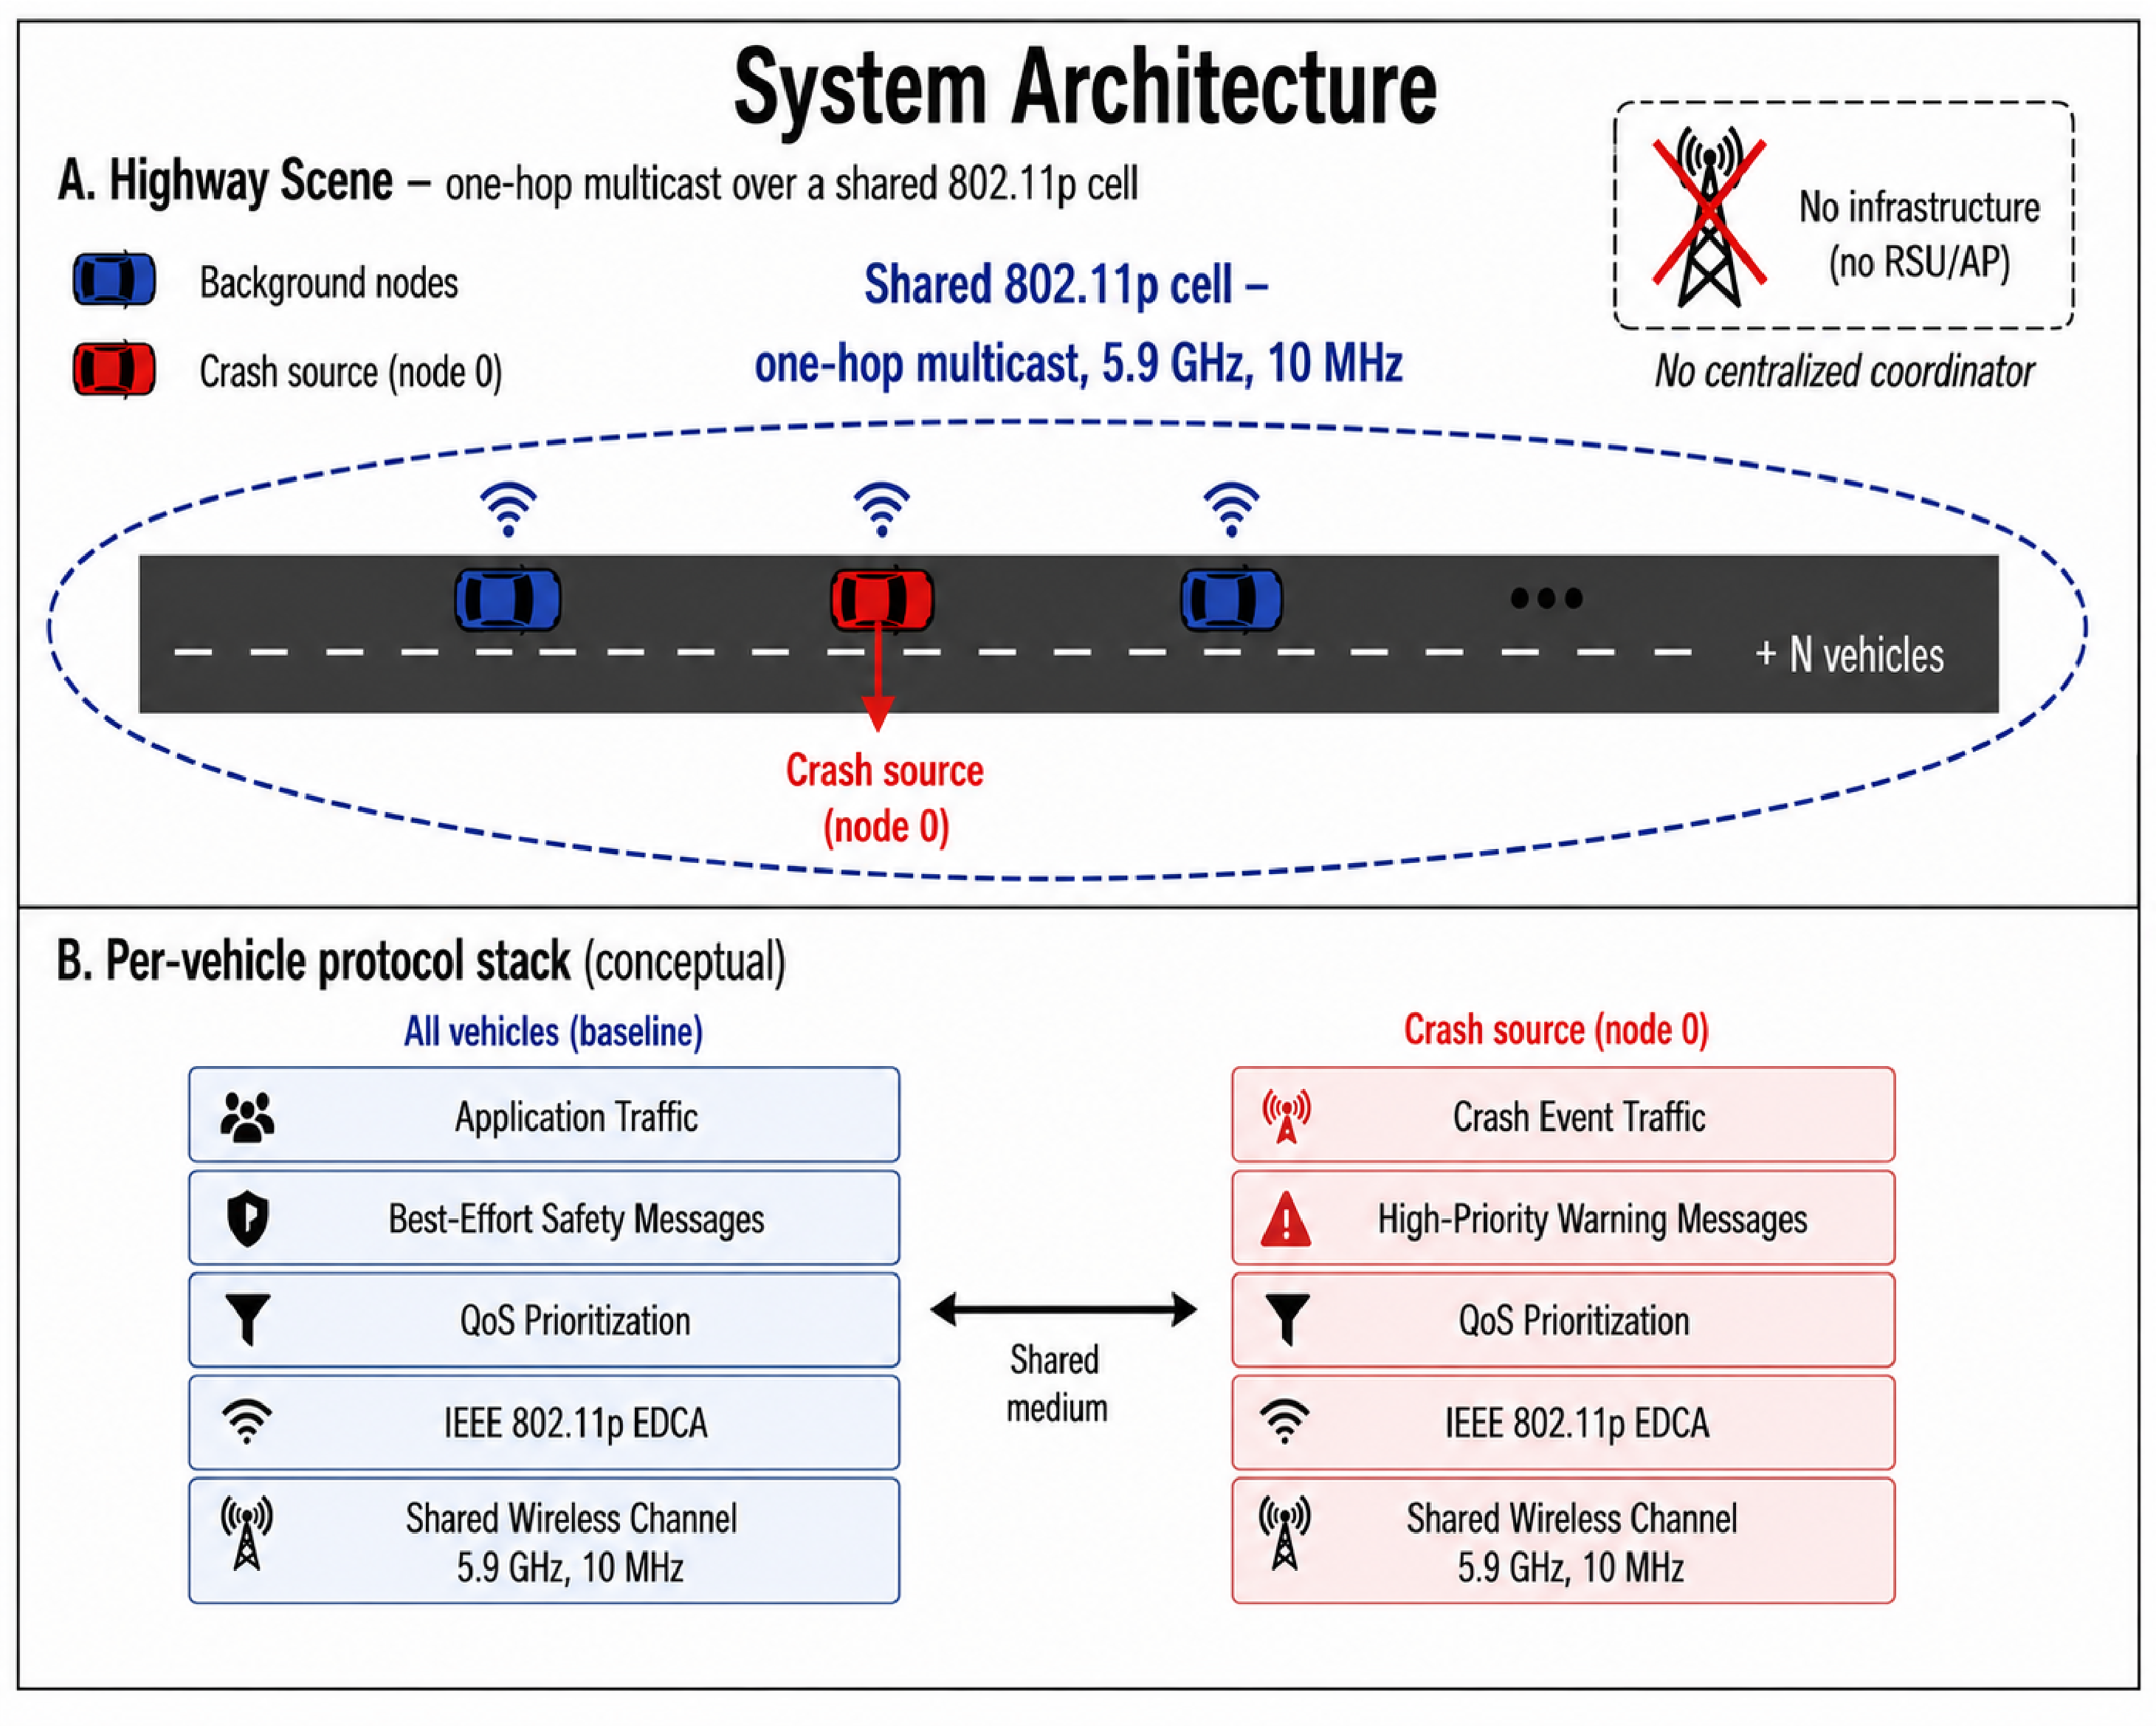
\includegraphics[width=0.92\linewidth]{Figs/system_model_architecture.pdf}
	\end{center}
	\fonte{Prepared by the author.}
\end{figure}

The radio model uses an IEEE~802.11p physical layer at 5.9~GHz with 10~MHz channelization; reference transmit power, channel index, sensitivity, noise floor, and \gls{snir} threshold are fixed for all policies and recorded with the implementation parameters in \autoref{tab:impl:parameters}.
Propagation is free-space path loss with binary obstruction and without small-scale fading or shadowing, as stated in \autoref{sec:sys:scope}.
\emph{Physical-layer connectivity is held fixed across the five \gls{mac} policies}, so differences between \gls{be} and \gls{vo} service reflect queueing and contention rather than time-varying link quality.
Dense highway broadcast already stresses this shared medium through repeated backoff freezing under load~\cite{Continuous_Backoff_Freezing_Li,bianchi2000DCF}; the model isolates that contention so that the policies can be compared under controlled offered load.

%%%%%%%%%%%%%%%%%%%%%%%%%%%%%%%%%%%%%%%%%%%%%%%%%%%%%%%%%%%%%%%%%%%%%%%%%%%%%%%%
\section{Traffic Model}
\label{sec:sys:traffic}

Traffic uses a synthetic two-class abstraction rather than standardized \gls{cam} or \gls{denm} schedules, ITS-G5 or WAVE application stacks, or production vehicular logic.
The goal is to isolate \gls{mac}-level protection-versus-cost trade-offs under controlled offered load, not to reproduce a complete \gls{its} protocol stack.

Every vehicle generates ordinary background traffic throughout the scenario horizon.
This flow represents non-critical cooperative traffic and is modeled by a configurable payload, a random inter-arrival process with a prescribed mean (exponential draws in the software artifact), and default Best Effort marking (\gls{dscp}~0).
The model instantiates this process with low, medium, and high offered-load profiles so all \gls{mac} policies face the same application-side load within a given profile; the concrete means, payloads, and Voice burst parameters appear in \autoref{tab:impl:parameters}.

Crash-alert dissemination is an event-driven overlay on that background.
One designated vehicle becomes the crash source at the configured crash time and begins emitting alert messages marked with \gls{dscp}~46, the Expedited Forwarding codepoint used in this study as the crash marker~\cite{RFC3246_EF_PHB,RFC4594_DiffServ_Service_Classes}.
Each logical alert may be repeated a configurable number of times, with configurable spacing and jitter, to represent short warning bursts.
Importantly, the crash-alert flow is \emph{superimposed} on the background flow rather than replacing it: the crash source continues to contribute ordinary \gls{be} traffic while simultaneously injecting urgent alerts.
After the crash window ends, alerts cease and the network returns to \gls{be}-only operation, as detailed in \autoref{sec:sys:event}.

%%%%%%%%%%%%%%%%%%%%%%%%%%%%%%%%%%%%%%%%%%%%%%%%%%%%%%%%%%%%%%%%%%%%%%%%%%%%%%%%
\section{QoS Model and MAC Policies}
\label{sec:sys:qos}

The model admits only two traffic classes.
Periodic background packets remain Best Effort and carry \gls{dscp}~0.
Crash-alert packets carry \gls{dscp}~46 and, in the \gls{qos}-enabled policies, are explicitly mapped to the IEEE~802.11 Voice user priority and \gls{ac}~\cite{RFC8325_WiFi_QoS,IEEE80211e_2005}.
That mapping is not automatic in every stack; the Background chapter's DiffServ path (\autoref{sec:bg:dscp}) is the normative mapping assumed here for QoS-enabled policies~\cite{RFC2474_DSField,RFC2475_DiffServ_Architecture}.
\autoref{fig:sys:stack} summarizes the abstract end-to-end path from application marking to channel access.

\begin{figure}[htb]
	\caption{\label{fig:sys:stack}Conceptual cross-layer path for crash-aware prioritization. Study-specific mechanisms act at Application, Network/\gls{qos}, and \gls{mac}; the shared \gls{phy} baseline is identical across all policies.}
	\begin{center}
		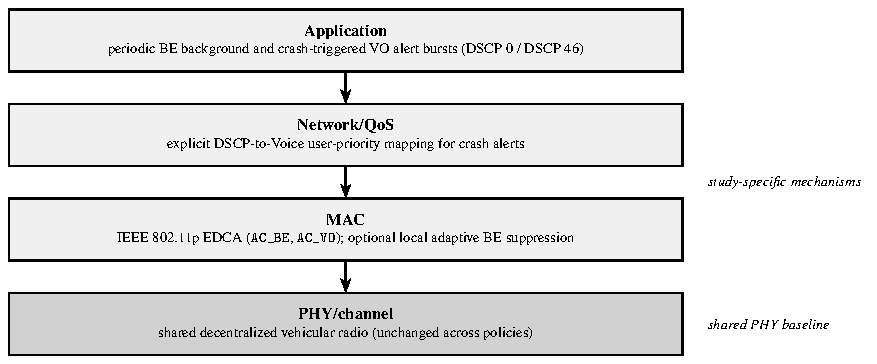
\includegraphics[width=0.95\linewidth]{Figs/sys_stack.pdf}
	\end{center}
	\fonte{Prepared by the author.}
\end{figure}

Five \gls{mac} policies operate on the same traffic and radio model.
They form a comparison ladder from undifferentiated access, through standard \gls{edca} differentiation, to three adaptive extensions that temporarily suppress competing \gls{be} traffic while crash alerts are active.
None of the policies reserves the channel or claims deterministic delay bounds: \gls{edca} provides statistical differentiation only~\cite{mangold2003QoS,kosekszott2012What,kong2004EDCA}.

\begin{itemize}
  \item \texttt{plain} --- Non-\gls{qos} \gls{dcf} baseline: undifferentiated access with a single pending queue and no DSCP-to-\gls{ac} mapping~\cite{IEEE80211,bianchi2000DCF}.
  \item \texttt{edca\_only} --- Standard \gls{qos} baseline: \gls{dscp}~46 maps to \texttt{AC\_VO}; all other packets use user priority~0~\cite{IEEE80211e_2005}.
  \item \texttt{edca\_v2x\_vo\_stable} --- Sustained Voice protection: inherits \texttt{edca\_only} and adds the adaptive controller below with comparatively long protection windows.
  \item \texttt{edca\_v2x\_vo\_guarded} --- Bounded suppression: same inheritance with tighter, shorter protection windows.
  \item \texttt{edca\_v2x\_vo\_emergency} --- Emergency preemption: same inheritance with aggressive activation; newly arriving \gls{be} packets may be dropped while protection is active.
\end{itemize}

\noindent
For brevity the adaptive policies are often abbreviated \texttt{stable}, \texttt{guarded}, and \texttt{emergency}.
Queue depths, contention windows, and controller timing knobs for each policy are bound in the implementation and listed in \autoref{tab:impl:parameters}.

\subsection{Adaptive three-mode controller}
\label{sec:sys:controller}

The three adaptive policies add a local three-mode \gls{fsm}---\emph{listening}, \emph{blocking}, and \emph{sending}---that temporarily gates \gls{be} eligibility for channel access without changing the underlying queue parameters inherited from \texttt{edca\_only}.
\autoref{fig:sys:fsm} summarizes the modes and transitions.

\begin{figure}[htb]
	\caption{\label{fig:sys:fsm}Local adaptive controller modes and transitions for the \texttt{edca\_v2x\_vo\_*} policies.}
	\begin{center}
		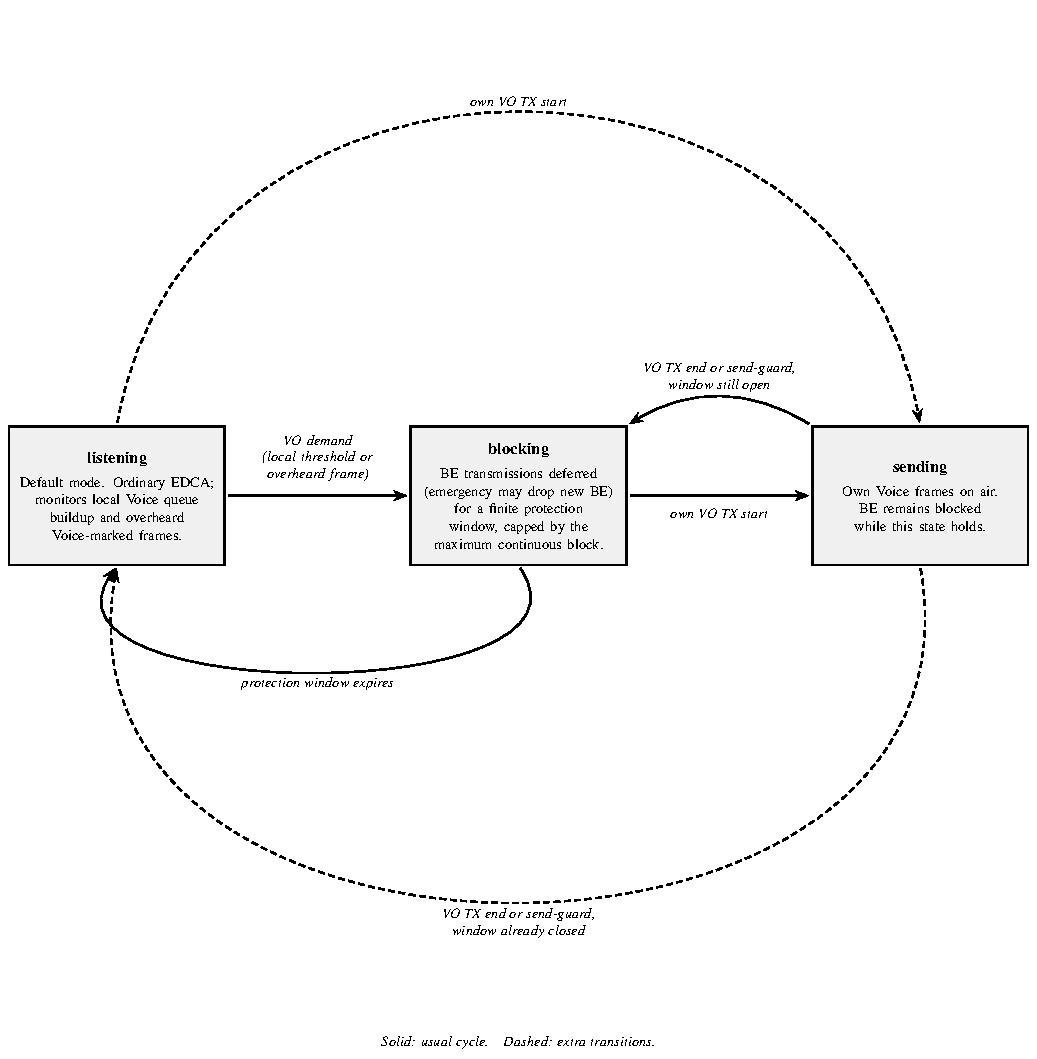
\includegraphics[width=0.95\linewidth]{Figs/sys_fsm.pdf}
	\end{center}
	\fonte{Prepared by the author.}
\end{figure}

A node leaves \emph{listening} for \emph{blocking} when the local Voice queue crosses the activation threshold or when any Voice-marked frame is overheard---a single overheard alert frame suffices to arm or extend protection; the queue threshold applies only to locally generated Voice traffic.
It moves to \emph{sending} when its own Voice frames obtain the channel.
After the Voice transmission ends---or if the send-guard timer fires first---it returns to \emph{blocking} while the protection window is still open, and to \emph{listening} once that window has expired.
Nodes that only overhear Voice traffic never enter \emph{sending}: they remain in \emph{blocking} until the window expires.
\autoref{fig:sys:fsm} also shows a skip from \emph{listening} directly to \emph{sending} when a local Voice frame wins the channel without a prior demand-triggered block.
Under \texttt{stable} and \texttt{guarded}, \gls{be} packets remain queued but lose channel-access eligibility while the controller is blocking or sending.
Under \texttt{emergency}, newly arriving \gls{be} packets may additionally be dropped and stale \gls{be} transmission opportunities released.
The mechanism shapes local contention during the alert period; it does \emph{not} reserve the medium, open scheduled gates, or provide worst-case latency bounds~\cite{IEEE80211e_2005,kosekszott2012What}.

%%%%%%%%%%%%%%%%%%%%%%%%%%%%%%%%%%%%%%%%%%%%%%%%%%%%%%%%%%%%%%%%%%%%%%%%%%%%%%%%
\section{Event Model}
\label{sec:sys:event}

The system evolves through three phases, illustrated in \autoref{fig:sys:timeline}.

\begin{figure}[htb]
	\caption{\label{fig:sys:timeline}Conceptual event timeline: normal background traffic, crash-triggered Voice prioritization, and recovery.}
	\begin{center}
		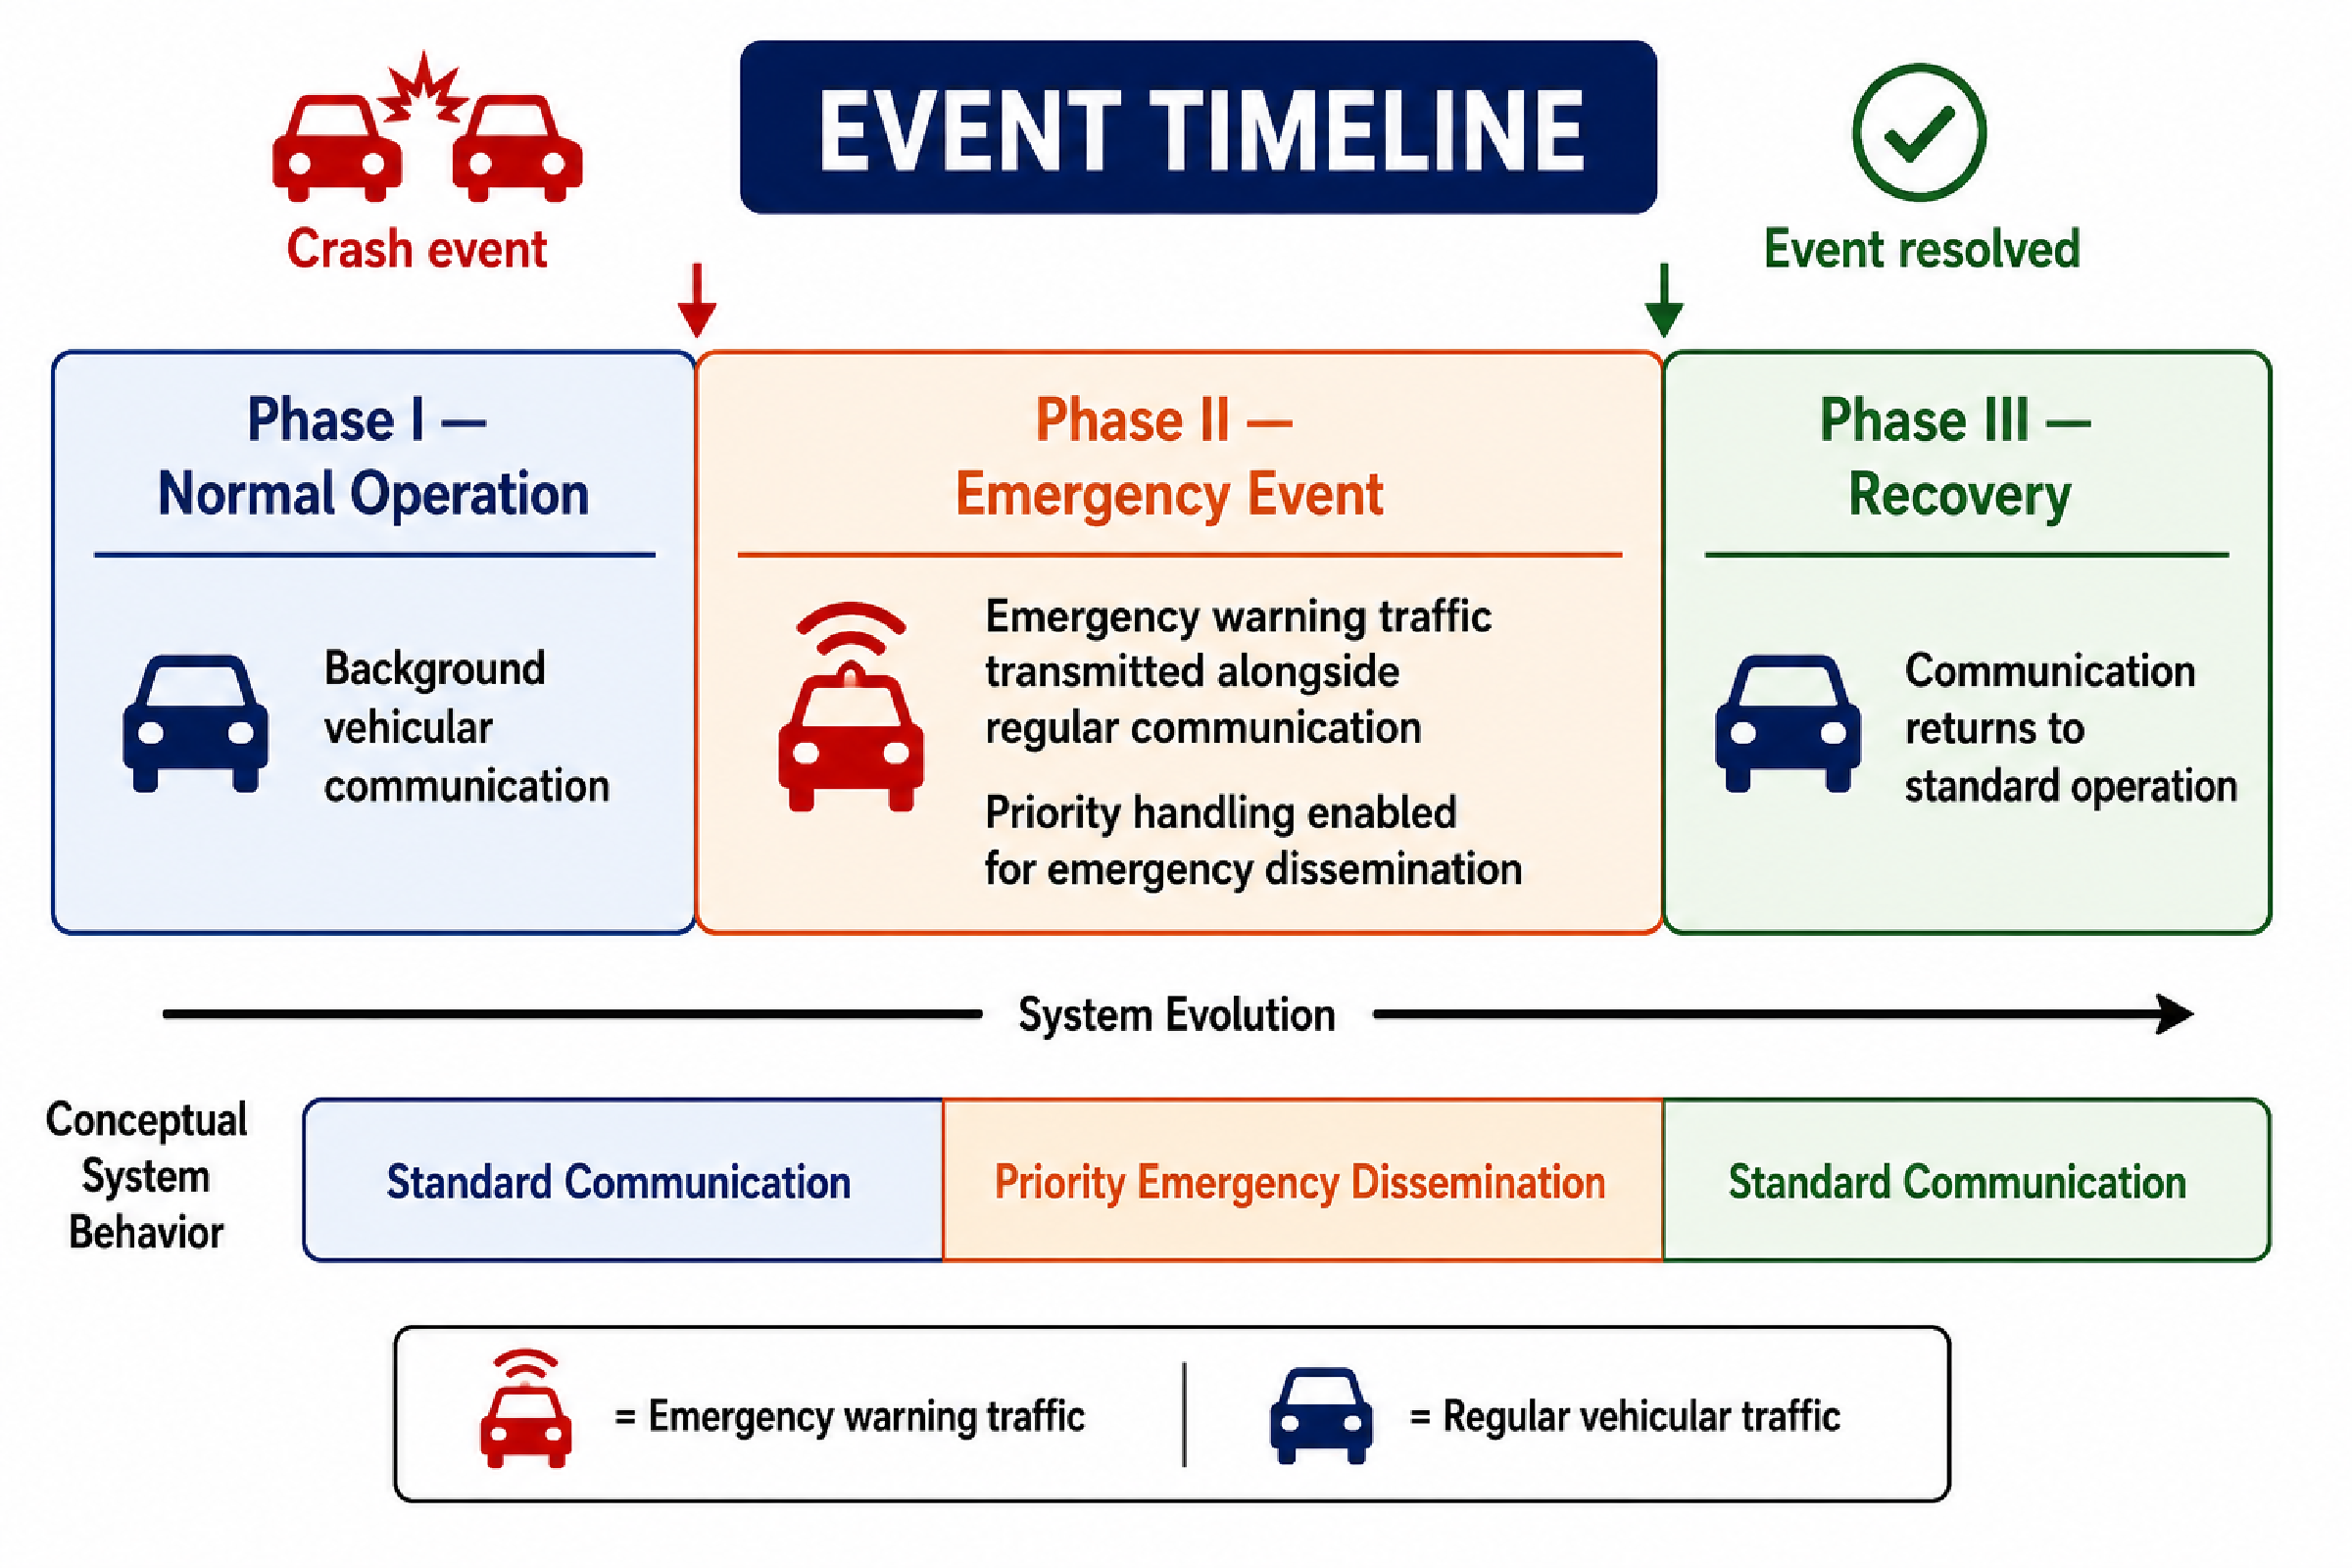
\includegraphics[width=\linewidth]{Figs/event_timeline_cropped.pdf}
	\end{center}
	\fonte{Prepared by the author.}
\end{figure}

\begin{enumerate}
  \item \textbf{Normal operation.}
    Before the crash event, all vehicles generate only periodic \gls{be} multicast traffic.
    No crash-alert Voice flow is present, and adaptive controllers remain in \emph{listening}.
  \item \textbf{Crash window.}
    At time~\SI{30}{\second} of the scenario horizon, one designated vehicle enters the crash state: it becomes stationary and immediately begins the Voice alert flow for a~\SI{30}{\second} window.
    Ordinary background traffic remains active across the network, including at the crash source, so urgent packets must compete with existing channel load~\cite{RFC9119_Multicast_IEEE802_Wireless}.
  \item \textbf{Recovery.}
    After the crash window expires, crash-alert transmissions cease and the system reverts to \gls{be}-only background traffic.
    Under the adaptive policies, however, the local effect of the crash can briefly outlast the application burst: nodes that still observe Voice queue pressure or receive crash-related Voice frames may remain temporarily in \emph{blocking} or \emph{sending} until the protection window and its short guard interval expire.
\end{enumerate}

This three-phase structure is deliberately simple.
It isolates a single crash source and a bounded alert interval so that the five policies can be compared on the same timeline under light and heavy fleet densities.

%%%%%%%%%%%%%%%%%%%%%%%%%%%%%%%%%%%%%%%%%%%%%%%%%%%%%%%%%%%%%%%%%%%%%%%%%%%%%%%%
\section{Assumptions and Scope}
\label{sec:sys:scope}

The model is intentionally minimal.
There is no infrastructure, centralized scheduler, or Time-Sensitive Networking-style gating; there is a single crash source; and there is a two-class \gls{be}/\gls{vo} distinction only.
Road geometry, fleet density, and radio parameters fix concrete instances of the model; their reference values are recorded with the implementation in \autoref{tab:impl:parameters}.

\gls{dcc}, as standardized for ITS-G5 deployments, is \emph{not} part of the model: application transmit rates follow the fixed offered-load profiles rather than reacting to channel busy ratio~\cite{etsi_dcc_2018}.
As argued in \autoref{sec:rel_work}, DCC remains a complementary always-on regulator; excluding it here isolates the protection-versus-cost behaviour of the five \gls{mac} policies.

Small-scale fading, log-normal shadowing, and graded obstacle attenuation are likewise omitted.
Connectivity uses free-space path loss, a static \gls{snir} threshold, and binary obstruction (a link is either clear or fully blocked).
Contention is therefore induced mainly by multicast load and fleet density, so the policies compete on backoff, queue service, and local \gls{be} suppression rather than on cross-layer load regulation or time-varying \gls{phy} stress.

Finally, the model makes no deterministic or worst-case latency claims.
\gls{edca} and all five policies provide statistical service only~\cite{kosekszott2012What,mangold2003QoS}.
Any quantitative statements about Voice or Best Effort delay belong to the evaluation, not to closed-form bounds derived from this chapter.

Together, the network, traffic, \gls{qos}, event, and scope definitions constitute the crash-aware system studied in the remainder of this dissertation.
\autoref{chap:implementation} maps the model onto a concrete software realization and records the numeric parameter bindings used in the artifact; the evaluation then asks whether crash-triggered Voice traffic obtains better wireless service than ordinary Best Effort under contention, and what cost that protection imposes on ordinary traffic.

% ---

% ---
% 4 -Capítulo 4
% ---
%\phantompart
\chapter{Implementation}
\label{chap:implementation}

\autoref{chap:sysmodel} defined the crash-aware system at a conceptual level: a decentralized IEEE~802.11p highway network, a synthetic two-class \gls{be}/\gls{vo} traffic model, five \gls{mac} policies with a local three-mode controller, and a three-phase crash timeline.
This chapter maps that model onto the concrete software artifact developed for this dissertation, so that a reader who already understands the design can reproduce the build, follow the packet path, and locate every study-specific module without consulting undocumented source comments.

The realization is an \gls{omnet}~6.1~\cite{varga2008omnetpp} / \gls{inet}~4.5.4~\cite{inet_framework} / Veins~5.3.1~\cite{veins_sommer2011} project whose source, scenario packages, and analysis tooling are publicly available~\cite{aguiar2026_veins_qos}.
Road mobility is provided by \gls{sumo} coupled through \gls{traci}~\cite{lopez2018sumo}.
The chapter is organized as follows.
Section~\ref{sec:impl:toolchain} pins the toolchain and repository layout.
Section~\ref{sec:impl:host} describes the vehicle host and scenario compound modules.
Section~\ref{sec:impl:path} traces the end-to-end packet path.
Section~\ref{sec:impl:apps} details the application modules.
Section~\ref{sec:impl:classifier} covers the DSCP-to-Voice classifier.
Section~\ref{sec:impl:mac} explains the instrumented \gls{mac} and the adaptive \gls{hcf} controller.
Section~\ref{sec:impl:policies} documents how the five policies are wired in configuration.
Section~\ref{sec:impl:scenarios} presents the highway scenario packages, the consolidated simulation-parameter table, and the configuration matrix.
Section~\ref{sec:impl:instrumentation} lists recorded signals and the analysis tooling surface.
Section~\ref{sec:impl:scope} states implementation scope and deliberate omissions.
Seeds, statistical aggregation, and measured results belong to \autoref{chap:evaluation} and are not reported here.

%%%%%%%%%%%%%%%%%%%%%%%%%%%%%%%%%%%%%%%%%%%%%%%%%%%%%%%%%%%%%%%%%%%%%%%%%%%%%%%%
\section{Simulation Toolchain and Repository Layout}
\label{sec:impl:toolchain}

The Background chapter motivates bidirectional road-and-network coupling for inter-vehicle protocol studies (\autoref{sec:bg:sim}).
Here the same stack is pinned to the versions used for the experiments and narrowed to the modules that realize the System Model.

\subsection{Framework versions}
\label{sec:impl:versions}

\gls{omnet}~6.1 provides the discrete-event engine, component model, and \texttt{.ini}/\texttt{.ned} configuration system in which every vehicle node is assembled~\cite{varga2008omnetpp}.
\gls{inet}~4.5.4 supplies the Internet protocol stack, IEEE~802.11p-capable \gls{mac} and \gls{phy}, radio propagation abstractions, and the Hybrid Coordination Function (\gls{hcf}) into which the study's adaptive controller is substituted for selected policies~\cite{inet_framework,IEEE80211e_2005}.
Veins couples \gls{omnet}/\gls{inet} to \gls{sumo} through \gls{traci}, so highway mobility, lane discipline, and the crash-node stop command remain consistent with the road microsimulation~\cite{veins_sommer2011,lopez2018sumo}.
In the artifact tree, \texttt{inet/} and \texttt{veins/} are git submodules consumed as read-only frameworks, pinned to the \gls{inet}~4.5.4 and Veins~5.3.1 releases; the study-authored code lives under \texttt{veins\_qos/}~\cite{aguiar2026_veins_qos}.

\subsection{Repository layout}
\label{sec:impl:layout}

\autoref{tab:impl:layout} summarizes the directories that matter for implementation and reproducibility.
Only the active highway packages participate in the dissertation experiment matrix; older square and early highway packages remain in the tree as development history and are not part of the reported study~\cite{aguiar2026_veins_qos}.

\begin{table}[htb]
	\ABNTEXfontereduzida
	\caption{\label{tab:impl:layout}Artifact directory layout relevant to the crash-aware implementation.}
	\begin{center}
		\begin{tabularx}{\linewidth}{@{}>{\ttfamily\raggedright\arraybackslash}p{4.4cm} X@{}}
			\toprule
			\textbf{Path} & \textbf{Role} \\
			\midrule
			veins\_qos/src/traffic/ &
			  Study applications: \texttt{CritPacketSender}, \texttt{CrashBurstApp}. \\
			\addlinespace
			veins\_qos/src/qos/ &
			  Explicit DSCP-to-user-priority classifier. \\
			\addlinespace
			veins\_qos/src/mac/ &
			  Instrumented IEEE~802.11 \gls{mac}, adaptive \gls{hcf}, and \gls{fsm} controller. \\
			\addlinespace
			veins\_qos/src/veins\_inet/ &
			  Veins$\leftrightarrow$\gls{inet} host, mobility, manager, and UDP application base. \\
			\addlinespace
			veins\_qos/simulations/veins\_inet\_highway\_\{light,heavy\}/ &
			  Active density packages: SUMO network, obstacles, \texttt{omnetpp.ini}, runners. \\
			\addlinespace
			kpi\_dashboard/ &
			  Offline parser of OMNeT++ \texttt{.sca}/\texttt{.vec} result files and figure export. \\
			\addlinespace
			inet/, veins/ &
			  Framework submodules (read-only). \\
			\bottomrule
		\end{tabularx}
	\end{center}
	\fonte{Prepared by the author.}
\end{table}

\subsection{Attribution}
\label{sec:impl:attribution}

The Veins/\gls{inet} integration modules under \texttt{veins\_qos/src/veins\_inet/} derive from the Veins project (Sommer et al.)~\cite{veins_sommer2011}.
The \texttt{VeinsInetTransparentMobility} component incorporates work by Jannusch Bigge (TU Dresden); it is present in the tree but is \emph{not} selected by the active highway configurations, which use \texttt{VeinsInetMobility} instead~\cite{aguiar2026_veins_qos}.
Study-specific logic is confined to the application generators, the classifier, the instrumented \gls{mac}, and---for the adaptive policies only---a replacement \gls{hcf} submodule, so that physical-layer connectivity, mobility, and offered-load profiles stay shared across all five \gls{mac} policies (\autoref{sec:sys:network}).

%%%%%%%%%%%%%%%%%%%%%%%%%%%%%%%%%%%%%%%%%%%%%%%%%%%%%%%%%%%%%%%%%%%%%%%%%%%%%%%%
\section{Host and Scenario Compound Modules}
\label{sec:impl:host}

\subsection{Vehicle host}
\label{sec:impl:car}

Each simulated vehicle is an instance of \texttt{veins\_qos.veins\_inet.VeinsInetCar}, a thin extension of INET's \texttt{AdhocHost} that carries a single IEEE~802.11 wireless interface (\texttt{wlan0}), an IPv4 stack with \texttt{HostAutoConfigurator}, and a Veins mobility submodule~\cite{inet_framework,aguiar2026_veins_qos}.
The manager launches cars with

\begin{quote}
\ttfamily *.manager.moduleType = "veins\_qos.veins\_inet.VeinsInetCar"
\end{quote}

so that every TraCI-injected node receives the same compound type.
Mobility is bound to \texttt{veins\_qos.veins\_inet.VeinsInetMobility}, which mirrors SUMO positions, headings, and presence into the INET mobility model~\cite{veins_sommer2011}.
IPv4 autoconfiguration joins the multicast group \texttt{224.0.0.1} on \texttt{wlan0}, matching the application destination used by both traffic generators.

\subsection{Application base}
\label{sec:impl:appbase}

Both study applications extend \texttt{VeinsInetApplicationBase}, itself derived from INET's \texttt{ApplicationBase} with Veins-aware \gls{udp} socket setup~\cite{inet_framework,aguiar2026_veins_qos}.
The base class opens a \gls{udp} socket on \texttt{wlan0}, disables multicast loopback (\texttt{setMulticastLoop(false)}), and provides helpers for timed transmission and TraCI access.
Study applications therefore inherit a common multicast send path and concentrate their own logic on marking, timing, and instrumentation.

\subsection{Scenario network}
\label{sec:impl:scenario-ned}

Each active package defines a \texttt{Scenario} network \gls{ned} that composes:

\begin{itemize}
  \item \texttt{Ieee80211DimensionalRadioMedium} --- shared radio medium for all nodes;
  \item \texttt{VeinsInetManager} --- TraCI scenario manager that launches SUMO through \texttt{veins\_launchd} on \texttt{localhost:9999} using \texttt{highway.launchd.xml};
  \item \texttt{PhysicalEnvironment} --- obstacle geometry from \texttt{highway.obstacles.xml};
  \item visualizers (optional for interactive runs);
  \item an initial \texttt{VeinsInetCar} placeholder; additional cars are injected by TraCI as SUMO vehicles appear.
\end{itemize}

This compound is the OMNeT++ \texttt{network} selected by every runnable configuration in the package~\cite{aguiar2026_veins_qos}.

%%%%%%%%%%%%%%%%%%%%%%%%%%%%%%%%%%%%%%%%%%%%%%%%%%%%%%%%%%%%%%%%%%%%%%%%%%%%%%%%
\section{End-to-End Packet Path}
\label{sec:impl:path}

\autoref{fig:impl:stack} and the steps below summarize how a packet moves from creation to KPI recording.
The path is identical for Best Effort and Voice except for DSCP marking, classifier mapping, and---under adaptive policies---\gls{hcf}-level Best Effort gating.

\begin{figure}[htb]
	\caption{\label{fig:impl:stack}Implemented cross-layer path from study applications to the shared radio. Adaptive \gls{hcf} modules appear only under the \texttt{edca\_v2x\_vo\_*} policies.}
	\begin{center}
	\ABNTEXfontereduzida
	\begin{tabularx}{\linewidth}{>{\centering\arraybackslash}X}
		\toprule
		\textbf{Application:} \texttt{CritPacketSender} (\gls{dscp}~0) or \texttt{CrashBurstApp} (\gls{dscp}~46); \texttt{CreationTimeTag}, optional sequence tag \\
		\midrule
		$\downarrow$ \\
		\textbf{UDP / IPv4:} multicast to \texttt{224.0.0.1} on \texttt{wlan0} (Crash destPort~9001; Crit local/dest~9001) \\
		\midrule
		$\downarrow$ \\
		\textbf{Classifier (EDCA policies):} \texttt{QosClassifier} maps \gls{dscp}~46~$\rightarrow$~\gls{up} Voice; others~$\rightarrow$~\gls{up}~0 \\
		\midrule
		$\downarrow$ \\
		\textbf{\gls{mac}:} \texttt{V2xIeee80211Mac}; \texttt{plain} uses \gls{dcf}; EDCA uses stock \texttt{Hcf} or \texttt{V2xHcf} \\
		\midrule
		$\downarrow$ \\
		\textbf{\gls{phy}:} \texttt{Ieee80211DimensionalRadio}, free-space path loss, \texttt{IdealObstacleLoss}, static \gls{snir} \\
		\midrule
		$\downarrow$ \\
		\textbf{Reception KPIs:} \texttt{CritPacketSender} on every node (port~9001) records BE/VO RX and delay \\
		\bottomrule
	\end{tabularx}
	\end{center}
	\fonte{Prepared by the author.}
\end{figure}

\begin{enumerate}
  \item The sending application creates a UDP payload, attaches a \texttt{CreationTimeTag} (and, for crash bursts, a sequence request), and marks the packet with a \texttt{DscpReq} of~0 or~46.
  \item \texttt{VeinsInetApplicationBase::sendPacket} delivers the frame to UDP, which sends to multicast \texttt{224.0.0.1}.
  \item IPv4 forwards onto \texttt{wlan0}. Under EDCA policies, \texttt{QosClassifier} converts DSCP into a \texttt{UserPriorityReq} before the frame enters the IEEE~802.11 \gls{mac}~\cite{RFC8325_WiFi_QoS}.
  \item \texttt{V2xIeee80211Mac} either enqueues into a single \gls{dcf} pending queue (\texttt{plain}) or into \gls{edca} access-category queues (\texttt{edca\_*}). Adaptive policies consult \texttt{V2xEdcaFsmController} before granting Best Effort channel access~\cite{IEEE80211e_2005}.
  \item The dimensional 802.11p radio transmits on the shared medium; receivers reverse the path through \gls{phy}, \gls{mac}, IP, and UDP.
  \item Every node's \texttt{CritPacketSender} (\texttt{app[0]}, port~9001) processes received datagrams, classifies them by DSCP into BE or VO KPI streams, skips self-originated addresses, and optionally deduplicates Voice repeats.
\end{enumerate}

Crash-alert frames are therefore generated by \texttt{CrashBurstApp} but counted at receivers by \texttt{CritPacketSender}, because the crash application sends to destination port~9001---the same port on which every vehicle listens for cooperative traffic~\cite{aguiar2026_veins_qos}.

%%%%%%%%%%%%%%%%%%%%%%%%%%%%%%%%%%%%%%%%%%%%%%%%%%%%%%%%%%%%%%%%%%%%%%%%%%%%%%%%
\section{Application Layer}
\label{sec:impl:apps}

Two custom application modules implement the synthetic traffic model of \autoref{sec:sys:traffic}.
Both are instantiated on every vehicle (\texttt{numApps = 2}); only the configured crash target activates the Voice overlay.

\subsection{\texttt{CritPacketSender}: periodic Best Effort}
\label{sec:impl:crit}

\texttt{veins\_qos.traffic.CritPacketSender} extends \texttt{VeinsInetApplicationBase} and generates the ordinary background flow~\cite{aguiar2026_veins_qos}.
\autoref{tab:impl:crit} lists the principal NED parameters and recorded statistics.

\begin{table}[htb]
	\ABNTEXfontereduzida
	\caption{\label{tab:impl:crit}Principal parameters and statistics of \texttt{CritPacketSender}.}
	\begin{center}
		\begin{tabularx}{\linewidth}{@{}>{\raggedright\arraybackslash}p{3.6cm} X@{}}
			\toprule
			\textbf{Item} & \textbf{Role in the artifact} \\
			\midrule
			\texttt{sendInterval}, \texttt{payloadBytes} &
			  Periodic offered load; overridden by \texttt{\_netload\_*} overlays. \\
			\addlinespace
			\texttt{dscp} (default~0) &
			  Best Effort marking carried as \texttt{DscpReq}. \\
			\addlinespace
			\texttt{localPort}/\texttt{destPort} (9001) &
			  UDP endpoints for BE TX and for all BE/VO RX KPIs. \\
			\addlinespace
			\texttt{voDedupWindow} &
			  Enables run-long Voice deduplication keyed by (source,~sequence); the time-valued name is retained for legacy configs, but entries are not mid-run expired. \\
			\addlinespace
			Statistics &
			  \texttt{beTxPackets}, \texttt{beRxPackets}, \texttt{voRxPackets}, \texttt{beEndToEndDelay}, \texttt{voEndToEndDelay} (vector + count/mean/min/max). \\
			\bottomrule
		\end{tabularx}
	\end{center}
	\fonte{Prepared by the author.}
\end{table}

On transmission, the module stamps \texttt{CreationTimeTag} and emits a Best Effort counter.
On reception it ignores datagrams whose Layer-3 source equals the local \texttt{wlan0} address, maps remaining packets by DSCP into BE or VO delay/RX streams, and---when deduplication is enabled---accepts only the first Voice packet of each (source,~sequence) pair for the remainder of the run.
This design keeps a single receiver module as the KPI sink for both traffic classes.

\subsection{\texttt{CrashBurstApp}: crash-triggered Voice}
\label{sec:impl:crash}

\texttt{veins\_qos.traffic.CrashBurstApp} implements the crash-alert overlay~\cite{RFC3246_EF_PHB,aguiar2026_veins_qos}.
Every vehicle instantiates the module, but only the node whose OMNeT++ index equals \texttt{targetNodeIndex} (default~0) schedules crash behaviour; the sentinel value~$-1$ would activate all nodes and is unused in the active matrix.

At absolute simulation time \texttt{crashAt} (30~s in the highway packages), the target node:

\begin{enumerate}
  \item marks itself visually (red icon) for interactive inspection;
  \item commands SUMO through TraCI to set speed to zero, realizing the stationary crash source of \autoref{sec:sys:event}~\cite{veins_sommer2011,lopez2018sumo};
  \item begins emitting Voice bursts marked with DSCP~46, each logical sequence comprising \texttt{repeatCount} physical packets spaced by \texttt{repeatGap} with optional \texttt{repeatJitter}.
\end{enumerate}

After \texttt{resumeAfter} (30~s), Voice transmission stops and TraCI restores normal speed control (\texttt{setSpeed(-1)}).
The crash source continues to run \texttt{CritPacketSender} throughout, so alerts are superimposed on ongoing Best Effort traffic rather than replacing it (\autoref{sec:sys:traffic}).

\autoref{tab:impl:crash} summarizes the crash-application surface.
Physical Voice transmissions increment \texttt{voTxPackets}; each logical burst sequence increments \texttt{voLogicalTxPackets}.
The evaluation prefers logical TX when present so that repeatCount does not inflate the denominator of reception ratios; the implementation exposes both counters precisely for that reason~\cite{aguiar2026_veins_qos}.

\begin{table}[htb]
	\ABNTEXfontereduzida
	\caption{\label{tab:impl:crash}Principal parameters and statistics of \texttt{CrashBurstApp}.}
	\begin{center}
		\begin{tabularx}{\linewidth}{@{}>{\raggedright\arraybackslash}p{3.6cm} X@{}}
			\toprule
			\textbf{Item} & \textbf{Role in the artifact} \\
			\midrule
			\texttt{targetNodeIndex} &
			  Which OMNeT++ node becomes the crash source (default~0). \\
			\addlinespace
			\texttt{crashAt}, \texttt{resumeAfter} &
			  Absolute crash start and crash-window duration. \\
			\addlinespace
			\texttt{sendInterval}, \texttt{payloadBytes} &
			  Inter-burst period and payload during the window. \\
			\addlinespace
			\texttt{repeatCount}, \texttt{repeatGap}, \texttt{repeatJitter} &
			  Physical repeats of each logical alert. \\
			\addlinespace
			\texttt{localPort}~9002 / \texttt{destPort}~9001 &
			  TX on a dedicated local port; RX KPIs collected by Crit on~9001. \\
			\addlinespace
			Statistics &
			  \texttt{voTxPackets} (physical), \texttt{voLogicalTxPackets} (per sequence). \\
			\bottomrule
		\end{tabularx}
	\end{center}
	\fonte{Prepared by the author.}
\end{table}

There is no multi-level criticality ladder and no separate four-priority application family: the implementation stays on the two-class \gls{be}/\gls{vo} abstraction fixed in the System Model.

%%%%%%%%%%%%%%%%%%%%%%%%%%%%%%%%%%%%%%%%%%%%%%%%%%%%%%%%%%%%%%%%%%%%%%%%%%%%%%%%
\section{QoS Classifier}
\label{sec:impl:classifier}

Correct placement of crash alerts into the Voice access category is not automatic under the common three-MSB DSCP-to-\gls{up} heuristic (\autoref{sec:bg:rfc8325}, \autoref{sec:sys:qos}).
The artifact therefore installs an explicit classifier rather than relying on default DiffServ-to-802.11 mapping~\cite{RFC8325_WiFi_QoS}.

\texttt{veins\_qos.qos.QosClassifier} implements INET's \texttt{IIeee8021dQosClassifier} interface.
It reads DSCP from packet indications or requests (and, if needed, from IPv4/IPv6 headers), maps \texttt{crashDscp} (default~46) to Voice user priority, and assigns \texttt{defaultUp} (default~0, Best Effort) to every other packet~\cite{RFC8325_WiFi_QoS,IEEE80211e_2005,aguiar2026_veins_qos}.
The resulting \texttt{UserPriorityReq} selects the corresponding \gls{edca} access category inside the \gls{hcf}.

The classifier is installed only under EDCA policies:

\begin{quote}
\ttfamily
*.node[*].wlan[*].classifier.typename = "veins\_qos.qos.QosClassifier"\\
*.node[*].wlan[*].classifier.crashDscp = 46\\
*.node[*].wlan[*].classifier.defaultUp = 0
\end{quote}

Under \texttt{plain}, no classifier is configured: a single \gls{dcf} pending queue carries all traffic without DSCP-to-\gls{ac} differentiation, matching the non-QoS baseline of \autoref{sec:sys:qos}.

%%%%%%%%%%%%%%%%%%%%%%%%%%%%%%%%%%%%%%%%%%%%%%%%%%%%%%%%%%%%%%%%%%%%%%%%%%%%%%%%
\section{MAC Layer: Instrumented MAC and Adaptive HCF}
\label{sec:impl:mac}

All active configurations replace the stock IEEE~802.11 \gls{mac} typename with an instrumented subclass, while only the adaptive policies replace the \gls{hcf} submodule~\cite{IEEE80211e_2005,inet_framework,aguiar2026_veins_qos}.

\subsection{\texttt{V2xIeee80211Mac}}
\label{sec:impl:v2xmac}

\texttt{veins\_qos.mac.V2xIeee80211Mac} extends INET's \texttt{Ieee80211Mac} and is selected globally:

\begin{quote}
\ttfamily *.node[*].wlan[*].mac.typename = "veins\_qos.mac.V2xIeee80211Mac"
\end{quote}

The module subscribes to \texttt{packetDroppedSignal} and, at finish time, records scalar drop totals partitioned by access category (BK, BE, VI, VO, and unclassified) and by drop reason (queue overflow, retry-limit reached, congestion, incorrectly received, and related INET reasons).
Those counters are the \gls{mac}-side counterpart to the application delay and reception statistics: they expose where frames were discarded under each policy without requiring Evaluation-side reinterpretation of raw event logs~\cite{aguiar2026_veins_qos}.

\subsection{\texttt{V2xHcf} and \texttt{V2xEdcaFsmController}}
\label{sec:impl:v2xhcf}

The adaptive policies substitute

\begin{quote}
\ttfamily *.node[*].wlan[*].mac.hcf.typename = "veins\_qos.mac.V2xHcf"
\end{quote}

for the stock INET \texttt{Hcf}.
\texttt{V2xHcf} implements the \texttt{IHcf} contract and embeds a full QoS \gls{hcf} submodule tree (EDCA, HCCA placeholder, originator/recipient QoS data services, rate selection, acknowledgement and RTS/CTS policies) plus a study-specific \texttt{FSMController} of type \texttt{V2xEdcaFsmController}~\cite{IEEE80211e_2005,aguiar2026_veins_qos}.
Because only the typename changes, queue depths and contention parameters inherited from \texttt{edca\_only} remain numerically identical across the adaptive profiles.

\autoref{tab:impl:v2xhcf} lists the controller-facing parameters declared on \texttt{V2xHcf} and its FSM submodule.
Their semantics match the three-mode controller of \autoref{sec:sys:controller}; this section records how those knobs are named in software.

\begin{table}[htb]
	\ABNTEXfontereduzida
	\caption{\label{tab:impl:v2xhcf}Adaptive controller parameters exposed by \texttt{V2xHcf} / \texttt{V2xEdcaFsmController}.}
	\begin{center}
		\begin{tabularx}{\linewidth}{@{}>{\ttfamily\raggedright\arraybackslash}p{4.0cm} X@{}}
			\toprule
			\textbf{Parameter} & \textbf{Meaning} \\
			\midrule
			adaptiveBlocking &
			  Enables Voice-driven Best Effort suppression through the FSM. \\
			\addlinespace
			emergencyPreemption &
			  When true, newly arriving Best Effort may be dropped and stale Best Effort grants suppressed while protection is active. \\
			\addlinespace
			blockDuration &
			  Protection-window extension per Voice demand event (local enqueue or overheard Voice frame). \\
			\addlinespace
			maxContinuousBlock &
			  Cap on one continuous blocking/sending interval (also mirrored on the FSM). \\
			\addlinespace
			voQueueThreshold &
			  Local Voice queue depth that can trigger protection from upper traffic. \\
			\addlinespace
			FSMController.sendingGuardTimeout &
			  Short guard that delays return to listening around Voice send transitions. \\
			\bottomrule
		\end{tabularx}
	\end{center}
	\fonte{Prepared by the author.}
\end{table}

\subsection{Controller integration hooks}
\label{sec:impl:hooks}

\autoref{tab:impl:hooks} summarizes how \texttt{V2xHcf} couples application- and peer-observed Voice activity to Best Effort eligibility.
The controller does not rewrite backoff arithmetic or introduce scheduled gates; it interposes on channel-access eligibility for Best Effort while Voice frames remain subject to ordinary \gls{edca} contention~\cite{IEEE80211e_2005}.

\begin{table}[htb]
	\ABNTEXfontereduzida
	\caption{\label{tab:impl:hooks}Principal integration hooks of \texttt{V2xHcf} relative to the stock INET \gls{hcf}.}
	\begin{center}
		\begin{tabularx}{\linewidth}{@{}>{\raggedright\arraybackslash}p{3.4cm} X@{}}
			\toprule
			\textbf{Hook} & \textbf{Behaviour in the adaptive policies} \\
			\midrule
			Voice demand detection &
			  Local Voice enqueue above \texttt{voQueueThreshold}, or an overheard Voice-classified \gls{mac} frame, calls into the FSM (\texttt{onVoDemandDetected}) and may start or extend a protection window of length \texttt{blockDuration}, capped by \texttt{maxContinuousBlock}. \\
			\addlinespace
			Upper-frame gating &
			  While the FSM reports Best Effort blocked (\emph{blocking} or \emph{sending}), Best Effort channel-access requests are deferred. \\
			\addlinespace
			Own Voice on air &
			  Start and end of the node's own Voice transmissions drive \texttt{onVoTransmissionStart}/\texttt{End}, moving the FSM through \emph{sending} and applying \texttt{sendingGuardTimeout} before listening resumes. \\
			\addlinespace
			Emergency preemption &
			  If \texttt{emergencyPreemption} is true, newly arriving Best Effort frames may be dropped with a congestion reason and stale Best Effort grants suppressed while protection is active. \\
			\addlinespace
			Instrumentation &
			  Signals/scalars \texttt{beDroppedWhileBlocked}, \texttt{beGrantSuppressedWhileBlocked}, and \texttt{voProtectionActivation}; FSM vector \texttt{v2xState} with encoding 0~=~listening, 1~=~blocking, 2~=~sending. \\
			\bottomrule
		\end{tabularx}
	\end{center}
	\fonte{Prepared by the author.}
\end{table}

%%%%%%%%%%%%%%%%%%%%%%%%%%%%%%%%%%%%%%%%%%%%%%%%%%%%%%%%%%%%%%%%%%%%%%%%%%%%%%%%
\section{MAC Policy Configuration Wiring}
\label{sec:impl:policies}

\autoref{tab:impl:map} restates the stack mapping.
The subsections below document the exact OMNeT++ configuration composition used in the active highway \texttt{omnetpp.ini} files~\cite{aguiar2026_veins_qos}.
Numeric access-control values are collected in \autoref{tab:impl:parameters}; here the emphasis is on \emph{which} typename and parameter paths bind them.

\begin{table}[htb]
	\ABNTEXfontereduzida
	\caption{\label{tab:impl:map}Artifact mapping per stack layer.}
	\begin{center}
		\begin{tabularx}{\linewidth}{@{}l >{\raggedright\arraybackslash}X >{\raggedright\arraybackslash}X@{}}
			\toprule
			\textbf{Layer} & \textbf{Reused baseline} & \textbf{Introduced modules} \\
			\midrule
			App. &
			  Multicast UDP hooks in \texttt{VeinsInetApplicationBase} &
			  \texttt{CritPacketSender}, \texttt{CrashBurstApp}; KPI tags and deduplication \\
			\addlinespace
			Net/\gls{qos} &
			  IPv4 forwarding and transport &
			  \texttt{QosClassifier} (\gls{dscp}~46~$\rightarrow$ Voice \gls{up}) \\
			\addlinespace
			\gls{mac} &
			  IEEE~802.11p \gls{dcf}/\gls{edca} queues and channel access &
			  \texttt{V2xIeee80211Mac}; \texttt{V2xHcf}+\texttt{V2xEdcaFsmController} on adaptive policies \\
			\addlinespace
			\gls{phy} &
			  Dimensional radio, propagation, mobility, TraCI coupling &
			  None (shared across all policies) \\
			\bottomrule
		\end{tabularx}
	\end{center}
	\fonte{Prepared by the author.}
\end{table}

\subsection{\texttt{plain}}
\label{sec:impl:plain}

\texttt{[Config plain]} keeps a non-QoS station.
It sets the single DCF pending-queue capacity to 128~packets and does not enable \texttt{qosStation}, does not install \texttt{QosClassifier}, and does not override \texttt{hcf.typename}.
DSCP markings still travel with IP packets for KPI classification at receivers, but they do not drive EDCA access categories.

\subsection{\texttt{edca\_only}}
\label{sec:impl:edca}

\texttt{[Config edca\_only]} extends the plain baseline with standard EDCA~\cite{IEEE80211e_2005}:

\begin{itemize}
  \item \texttt{mac.qosStation = true};
  \item \texttt{mac.hcf.typename = "Hcf"} (stock INET);
  \item \texttt{QosClassifier} as above;
  \item pending-queue capacities BK/BE/VI/VO = 128/128/64/32 (\texttt{edcaf[0..3]});
  \item MSDU aggregation policy cleared (\texttt{msduAggregationPolicy.typename = ""});
  \item \gls{aifsn} BK/BE/VI/VO = 7/3/2/2;
  \item \texttt{cwMin}/\texttt{cwMax} BK/BE = 15--1023, VI = 7--15, VO = 3--7.
\end{itemize}

INET indexes \texttt{edcaf[0]=BK}, \texttt{[1]=BE}, \texttt{[2]=VI}, \texttt{[3]=VO}; the active applications exercise only BE and VO, so VI/BK queues exist but remain empty under the two-class traffic model.

\subsection{Adaptive profiles}
\label{sec:impl:adaptive}

Each adaptive configuration extends \texttt{edca\_only}, replaces \texttt{hcf.typename} with \texttt{veins\_qos.mac.V2xHcf}, and sets \texttt{adaptiveBlocking = true}.
\autoref{tab:impl:policyknobs} records the profile-specific knobs exactly as bound in \texttt{omnetpp.ini}.

\begin{table}[htb]
	\ABNTEXfontereduzida
	\caption{\label{tab:impl:policyknobs}Adaptive policy knobs as bound in the highway \texttt{omnetpp.ini}.}
	\begin{center}
		\begin{tabularx}{\linewidth}{@{}l >{\raggedright\arraybackslash}X@{}}
			\toprule
			\textbf{Config} & \textbf{Controller binding} \\
			\midrule
			\texttt{edca\_v2x\_vo\_stable} &
			  \texttt{blockDuration=15ms}, \texttt{maxContinuousBlock=80ms}, \texttt{sendingGuardTimeout=5ms}, \texttt{voQueueThreshold=2}; \texttt{emergencyPreemption} left false. \\
			\addlinespace
			\texttt{edca\_v2x\_vo\_guarded} &
			  \texttt{blockDuration=4ms}, \texttt{maxContinuousBlock=20ms}, \texttt{sendingGuardTimeout=4ms}, \texttt{voQueueThreshold=3}; preemption false. \\
			\addlinespace
			\texttt{edca\_v2x\_vo\_emergency} &
			  \texttt{emergencyPreemption=true}, \texttt{blockDuration=10ms}, \texttt{maxContinuousBlock=60ms}, \texttt{sendingGuardTimeout=5ms}, \texttt{voQueueThreshold=1}. \\
			\bottomrule
		\end{tabularx}
	\end{center}
	\fonte{Prepared by the author.}
\end{table}

Legacy configuration names from earlier prototypes (for example Friendly/Protect aliases documented in the artifact's deprecation notes) are not part of the active matrix and must not be confused with the five policies of \autoref{sec:sys:qos}.

%%%%%%%%%%%%%%%%%%%%%%%%%%%%%%%%%%%%%%%%%%%%%%%%%%%%%%%%%%%%%%%%%%%%%%%%%%%%%%%%
\section{Scenario Packages, Simulation Parameters, and Configuration Matrix}
\label{sec:impl:scenarios}

\subsection{Consolidated simulation parameters}
\label{sec:impl:parameters}

\autoref{tab:impl:parameters} collects the concrete timing, topology, radio, application, classifier, and \gls{mac} bindings used by the active highway artifact.
It is the numeric counterpart of the System Model in \autoref{chap:sysmodel}: the conceptual roles of the five policies and the crash timeline are defined there; the values that instantiate them in this study are recorded here~\cite{aguiar2026_veins_qos}.
Best Effort inter-arrivals use OMNeT++ \texttt{exponential($\cdot$)} draws with the stated mean; Voice burst periods are fixed, with optional per-repeat jitter.
Adaptive policies are abbreviated \texttt{stable}, \texttt{guarded}, and \texttt{emergency} in the first column; the full OMNeT++ configuration names are \texttt{edca\_v2x\_vo\_*}.

\begin{table}[H]
	\ABNTEXfontereduzida
	\caption{\label{tab:impl:parameters}Simulation parameters used in the crash-aware Veins/\gls{inet} artifact.}
	\begin{center}
	\setlength{\tabcolsep}{3.5pt}
	\begin{tabularx}{\linewidth}{@{}
		>{\raggedright\arraybackslash}p{2.6cm}
		>{\raggedright\arraybackslash}p{2.9cm}
		>{\raggedright\arraybackslash}X
		@{}}
		\toprule
		\multicolumn{3}{@{}l@{}}{\textbf{Common highway setting}} \\
		\midrule
		\textbf{Parameter} & \textbf{Value} & \textbf{Notes} \\
		\midrule
		Sim.\ time &
		  \SI{70}{\second} &
		  \texttt{sim-time-limit}; identical for every configuration. \\
		\addlinespace
		Corridor &
		  5~km, 3+3 lanes &
		  Straight bidirectional SUMO corridor, three lanes per direction; mixed car/truck types (EIDM, LC2013); nominal lane speed \SI{120}{\km\per\hour}. \\
		\addlinespace
		Density &
		  10~/~100~veh. &
		  Light and heavy packages (\texttt{veins\_inet\_highway\_light}/\texttt{\_heavy}); same \texttt{omnetpp.ini}, different \texttt{highway.rou.xml}. \\
		\addlinespace
		Crash &
		  \SI{30}{\second}--\SI{60}{\second} &
		  Node index~0 (\texttt{node0\_highway}): TraCI stop, DSCP~46 alerts; BE background continues. \\
		\addlinespace
		Radio &
		  802.11p / ch.~3 &
		  5.9~GHz, 10~MHz, 20~mW; \texttt{Ieee80211DimensionalRadio}; mode~\texttt{p}; data frames at 12~Mbit/s (fastest mandatory mode, \gls{inet} default rate selection). \\
		\addlinespace
		Propagation &
		  FS~+~binary &
		  Free-space path loss; no fading/shadowing; \texttt{IdealObstacleLoss} + \texttt{highway.obstacles.xml}; SNIR~\SI{4}{\decibel}; sens.\ $-$85~dBm; noise $-$110~dBm (\gls{inet}~4.5.4 defaults, not overridden). \\
		\addlinespace
		Multicast &
		  \texttt{224.0.0.1} &
		  On \texttt{wlan0}. Crit ports 9001/9001; Crash local~9002, dest~9001 (VO RX counted in Crit). \\
		\addlinespace
		TraCI &
		  port~9999 &
		  \texttt{localhost}; \texttt{VeinsInetManager} + \texttt{veins\_launchd}; update~\SI{1}{\second}; SUMO step~\SI{0.1}{\second}. \\
		\addlinespace
		Host/\gls{mac} &
		  \texttt{VeinsInetCar} &
		  Always \texttt{V2xIeee80211Mac}; adaptive policies replace \texttt{Hcf} with \texttt{V2xHcf}. \\
		\addlinespace
		Classifier &
		  DSCP~46~$\rightarrow$~VO &
		  \texttt{QosClassifier} on EDCA policies only (\texttt{crashDscp=46}, \texttt{defaultUp=0}); unused under \texttt{plain}. \\
		\addlinespace
		Recording &
		  vec.\ +\ sca. &
		  \texttt{**.vector-recording}/\texttt{scalar-recording = true}. \\
		\addlinespace
		Matrix &
		  15~/~package &
		  Five policies $\times$ three loads; $\times$ two densities $=$ 30 named experiments before seeds. \\
		\midrule
		\multicolumn{3}{@{}l@{}}{\textbf{Application load profiles (\texttt{\_netload\_*})}} \\
		\midrule
		\textbf{Profile} & \textbf{BE (\texttt{app[0]})} & \textbf{VO crash (\texttt{app[1]})} \\
		\midrule
		\texttt{low} &
		  exp.~\SI{500}{\milli\second}, 200~B &
		  \SI{120}{\milli\second}, 150~B; repeat~3; gap~\SI{20}{\milli\second}; jitter~\SI{5}{\milli\second}. \\
		\addlinespace
		\texttt{medium} &
		  exp.~\SI{250}{\milli\second}, 320~B &
		  \SI{75}{\milli\second}, 180~B; repeat~4; gap~\SI{15}{\milli\second}; jitter~\SI{5}{\milli\second}. \\
		\addlinespace
		\texttt{high} &
		  exp.~\SI{125}{\milli\second}, 420~B &
		  \SI{20}{\milli\second}, 260~B; repeat~8; gap~\SI{5}{\milli\second}; jitter~\SI{2}{\milli\second}. \\
		\midrule
		\multicolumn{3}{@{}l@{}}{\textbf{\gls{mac} policies (runnable name \texttt{<policy>\_netload\_<profile>})}} \\
		\midrule
		\textbf{Policy} & \textbf{Role} & \textbf{Access-control parameters} \\
		\midrule
		\texttt{plain} &
		  Non-\gls{qos} \gls{dcf} &
		  Single pending queue~128; no classifier; no \gls{edca}; no adaptive blocking. \\
		\addlinespace
		\texttt{edca\_only} &
		  Stock EDCA &
		  \texttt{Hcf} + \texttt{QosClassifier}. DSCP~46~$\rightarrow$~\texttt{AC\_VO}, else UP~0. Queues BK/BE/VI/VO: 128/128/64/32. \gls{aifsn} 7/3/2/2. \texttt{cwMin} 15/15/7/3. \texttt{cwMax} 1023/1023/15/7. \\
		\addlinespace
		\texttt{stable} &
		  Sustained VO &
		  Config \texttt{edca\_v2x\_vo\_stable}. Inherits \texttt{edca\_only}; \texttt{V2xHcf}. Block~\SI{15}{\milli\second}; max cont.~\SI{80}{\milli\second}; guard~\SI{5}{\milli\second}; VO thr.~2. \\
		\addlinespace
		\texttt{guarded} &
		  Bounded VO &
		  Config \texttt{edca\_v2x\_vo\_guarded}. Same inheritance. Block~\SI{4}{\milli\second}; max cont.~\SI{20}{\milli\second}; guard~\SI{4}{\milli\second}; VO thr.~3. \\
		\addlinespace
		\texttt{emergency} &
		  Emergency VO &
		  Config \texttt{edca\_v2x\_vo\_emergency}; \texttt{emergencyPreemption=true}. Block~\SI{10}{\milli\second}; max cont.~\SI{60}{\milli\second}; guard~\SI{5}{\milli\second}; VO thr.~1; may drop BE. \\
		\bottomrule
	\end{tabularx}
	\end{center}
	\fonte{Prepared by the author.}
\end{table}

\subsection{Density packages}
\label{sec:impl:density}

The dissertation experiments use two parallel packages under
\texttt{veins\_qos/simulations/}~\cite{aguiar2026_veins_qos}:

\begin{itemize}
  \item \texttt{veins\_inet\_highway\_light} --- light-density corridor with 10~vehicles;
  \item \texttt{veins\_inet\_highway\_heavy} --- heavy-density corridor with 100~vehicles.
\end{itemize}

Both packages share the same corridor geometry (\texttt{highway.net.xml}), obstacle file, launchd description, and---byte-for-byte in the active tree---the same \texttt{omnetpp.ini}.
Fleet size is selected by the SUMO route file (\texttt{highway.rou.xml}): a fixed vehicle \texttt{node0\_highway} departs at time~0 and becomes OMNeT++ node index~0 (the default crash target), while additional vehicles are injected from SUMO flows.
Separating density (package) from offered load (ini overlay) is deliberate: the two stress dimensions can be varied independently~\cite{aguiar2026_veins_qos}.

\subsection{Road network and mobility}
\label{sec:impl:sumo}

The SUMO network is a straight bidirectional highway corridor of 5~km with three lanes per direction and mixed car/truck vehicle types under EIDM car-following and LC2013 lane-changing models~\cite{lopez2018sumo}.
Simulation step size is 0.1~s; teleportation on gridlock is disabled (\texttt{time-to-teleport=-1}) so that stopped crash nodes remain in place.
Veins updates network-node mobility from TraCI; the manager polls on a one-second update interval in the highway ini, while SUMO itself advances at its finer step~\cite{veins_sommer2011}.

\subsection{Radio and propagation baseline}
\label{sec:impl:radio}

Every configuration shares the IEEE~802.11p radio profile summarized in \autoref{tab:impl:parameters}~\cite{IEEE80211,inet_framework}:

\begin{itemize}
  \item operation mode \texttt{p}, band 5.9~GHz, channel~3, bandwidth 10~MHz, transmit power 20~mW;
  \item radio typename \texttt{Ieee80211DimensionalRadio};
  \item antenna mobility attached to the vehicle mobility module with a fixed longitudinal/height offset;
  \item obstacle loss typename \texttt{IdealObstacleLoss}, configured from
        \texttt{highway.obstacles.xml}~\cite{inet_ideal_obstacle_loss};
  \item free-space path loss and a static SNIR threshold, without small-scale fading or shadowing (\autoref{sec:sys:scope}).
\end{itemize}

Receiver sensitivity ($-$85~dBm), energy detection ($-$85~dBm), the \gls{snir} threshold (\SI{4}{\decibel}), background noise ($-$110~dBm), free-space path loss, and constant-speed propagation are the \gls{inet}~4.5.4 defaults for this radio and medium; they are not overridden in the configuration.
No rate-control module is configured, so \gls{inet}'s default rate selection transmits data frames---including group-addressed ones---at the fastest mandatory mode of the \SI{10}{\mega\hertz} \gls{ofdm} mode set (12~Mbit/s).
This differs from production deployments, where group-addressed frames are commonly sent at a basic rate (\autoref{sec:bg:multicast}); the choice is uniform across all five policies.

Two fidelity caveats apply.
First, the artifact realizes 802.11p-like operation through \gls{inet}'s \texttt{AdhocHost} (no association or authentication, ad hoc management); it approximates \gls{ocb} operation rather than literally implementing \texttt{dot11OCBActivated} behaviour.
Second, the \gls{edca} parameter set of \autoref{tab:impl:parameters} follows the IEEE~802.11 BSS QoS defaults, whereas IEEE~802.11 specifies a distinct default \gls{edca} parameter set for \gls{ocb} operation with a less aggressive Best Effort category (\gls{aifsn}~6 instead of~3)~\cite{IEEE80211,etsi_en_302663}.
The configured set therefore makes Best Effort compete harder than an \gls{ocb}-default deployment would, which is conservative for the protection problem studied here.

Because this baseline is identical across policies, cross-policy differences isolate queueing, contention, and local Best Effort suppression.

\subsection{Timing and default application binding}
\label{sec:impl:timing}

Under \texttt{[General]}, both packages set \texttt{sim-time-limit = 70s}, crash start \texttt{crashAt = 30s}, and crash duration \texttt{resumeAfter = 30s}, matching \autoref{sec:sys:event} and \autoref{tab:impl:parameters}.
Default application parameters in \texttt{[General]} match the medium load profile; the \texttt{\_netload\_*} overlays override them for the full matrix.

\subsection{Load overlays and runnable matrix}
\label{sec:impl:matrix}

Three helper configurations vary only application-side load, using the means and payloads in \autoref{tab:impl:parameters}.
Runnable experiments compose a policy configuration with a load overlay via OMNeT++ \texttt{extends}, for example

\begin{quote}
\ttfamily
[Config edca\_v2x\_vo\_emergency\_netload\_high]\\
extends = edca\_v2x\_vo\_emergency, \_netload\_high
\end{quote}

yielding the naming pattern \texttt{<policy>\_netload\_<low|medium|high>}: five policies $\times$ three loads $=$ fifteen named configurations per density package~\cite{aguiar2026_veins_qos}.
Across both light and heavy packages the unique named experiments therefore total thirty before seed repetitions (seed counts belong to Evaluation).

Batch execution helpers in each package (\texttt{run}, \texttt{run\_matrix.sh}) select profiles such as high-load-only cores or the full fifteen-config matrix; they presuppose a running \texttt{veins\_launchd} on port~9999.
Building the study library follows the standard OMNeT++ pattern (\texttt{make makefiles \&\& make} under \texttt{veins\_qos/}) with NED paths that include INET, Veins, and \texttt{veins\_inet} sources~\cite{aguiar2026_veins_qos}.

%%%%%%%%%%%%%%%%%%%%%%%%%%%%%%%%%%%%%%%%%%%%%%%%%%%%%%%%%%%%%%%%%%%%%%%%%%%%%%%%
\section{Instrumentation and Analysis Surface}
\label{sec:impl:instrumentation}

\subsection{Recorded signals}
\label{sec:impl:signals}

Highway configurations enable comprehensive recording:

\begin{quote}
\ttfamily **.vector-recording = true\\
**.scalar-recording = true
\end{quote}

\autoref{tab:impl:signals} collects the study-relevant statistics emitted by the modules described above.
These signals are the measurement surface consumed by Evaluation; their statistical treatment (seeds, pooling, confidence reporting) is deferred to that chapter.

\begin{table}[htb]
	\ABNTEXfontereduzida
	\caption{\label{tab:impl:signals}Study-relevant instrumentation exposed by the artifact.}
	\begin{center}
		\begin{tabularx}{\linewidth}{@{}l >{\raggedright\arraybackslash}X@{}}
			\toprule
			\textbf{Source} & \textbf{Recorded quantities} \\
			\midrule
			\texttt{CritPacketSender} &
			  BE TX/RX counts; VO RX counts; BE and VO end-to-end delay vectors with count/mean/min/max scalars. \\
			\addlinespace
			\texttt{CrashBurstApp} &
			  Physical VO TX count; logical VO sequence count. \\
			\addlinespace
			\texttt{V2xIeee80211Mac} &
			  Per-\gls{ac} drop totals; per-reason drop totals (overflow, retry limit, congestion, \ldots). \\
			\addlinespace
			\texttt{V2xHcf} &
			  Best Effort drops while blocked; Best Effort grant suppressions; Voice protection activations. \\
			\addlinespace
			\texttt{V2xEdcaFsmController} &
			  \texttt{v2xState} vector (listening/blocking/sending). \\
			\bottomrule
		\end{tabularx}
	\end{center}
	\fonte{Prepared by the author.}
\end{table}

End-to-end delay is computed at receivers as simulation time minus \texttt{CreationTimeTag}.
For crash frames the creation stamp is the actual send instant of each physical repeat, so delay reflects channel and queueing latency rather than logical inter-burst spacing~\cite{aguiar2026_veins_qos}.

\subsection{Offline analysis tooling}
\label{sec:impl:kpi}

The companion \texttt{kpi\_dashboard/} project parses OMNeT++ scalar and vector result files, caches intermediate tables, and exports publication figures~\cite{aguiar2026_veins_qos}.
From an implementation perspective its contract is:

\begin{itemize}
  \item ingest \texttt{.sca}/\texttt{.vec} outputs under each scenario's \texttt{results/} directory;
  \item aggregate application delays and counts from \texttt{Scenario.node[*].app[0]} (and crash TX from \texttt{app[1]});
  \item expose controller and drop counters when present under adaptive policies;
  \item write tabular and figure artifacts consumed by Evaluation.
\end{itemize}

The dashboard does not alter simulation behaviour; it is a reproducibility aid that turns the instrumentation of \autoref{tab:impl:signals} into analysis-ready products.
Interpretation of those products---protection-versus-cost trade-offs, confidence intervals, and discussion---belongs to the Evaluation chapter.

%%%%%%%%%%%%%%%%%%%%%%%%%%%%%%%%%%%%%%%%%%%%%%%%%%%%%%%%%%%%%%%%%%%%%%%%%%%%%%%%
\section{Implementation Scope and Deliberate Omissions}
\label{sec:impl:scope}

The code base stays aligned with the minimal System Model of \autoref{sec:sys:scope}:

\begin{itemize}
  \item a single crash source and a two-class \gls{be}/\gls{vo} distinction only;
  \item no infrastructure, roadside unit, or Time-Sensitive Networking-style gating;
  \item no \gls{dcc} rate control---application rates follow the fixed offered-load overlays;
  \item no multi-crash orchestration and no standardized CAM/DENM stack;
  \item no small-scale fading, shadowing, or graded obstacle attenuation beyond binary \texttt{IdealObstacleLoss}~\cite{inet_ideal_obstacle_loss}.
\end{itemize}

Older packages under \texttt{simulations/veins\_inet\_square/},
\texttt{veins\_inet\_highway/}, and \texttt{veins\_inet\_light/}
are retained for development history and must not be mixed with the active light/heavy highway result trees when analysing the dissertation campaigns~\cite{aguiar2026_veins_qos}.

Together, the toolchain, host compounds, packet path, applications, classifier, instrumented \gls{mac}, adaptive \gls{hcf}, policy wiring, scenario packages, and instrumentation constitute the concrete realization of the crash-aware System Model.
\autoref{chap:evaluation} asks whether crash-triggered Voice traffic obtains better wireless service than ordinary Best Effort under contention, and what cost that protection imposes on ordinary traffic.


% ---
% 5 - Evaluation
% ---
\chapter{Evaluation}
\label{chap:evaluation}

\autoref{chap:sysmodel} defined the crash-aware system conceptually, and \autoref{chap:implementation} mapped it onto the Veins/\gls{inet} artifact.
This chapter asks whether that realization works as intended: does crash-triggered Voice traffic obtain better wireless service than ordinary Best Effort under contention, and what cost does that protection impose on ordinary traffic?

The evaluation is a protection-versus-cost study, not a claim of deterministic real-time guarantees~\cite{kosekszott2012What,IEEE80211e_2005}.
Two highway-density packages are used: a light-density sensitivity sweep (10~vehicles) and a heavy-density congestion stress case (100~vehicles), with emphasis on the latter~\cite{aguiar2026_veins_qos}.
Numeric bindings for timing, radio, load, and \gls{mac} policies are those of \autoref{tab:impl:parameters}; this chapter reports outcomes, not module wiring.

The chapter is organized as follows.
Section~\ref{sec:eval:setup} states the experimental matrix and seed budgets.
Section~\ref{sec:eval:metrics} defines metrics and aggregation.
Section~\ref{sec:eval:headline} states the headline answer and the two enabling conditions.
Section~\ref{sec:eval:hotspot} presents the primary positive result: Voice recovery under \texttt{hotspot\_high}.
Section~\ref{sec:eval:light} records the uniform-load null case that makes that result conditional.
Section~\ref{sec:eval:cost} prices the Best Effort cost of protection.
Section~\ref{sec:eval:discussion} discusses interpretation, practical significance, and limitations.
Section~\ref{sec:eval:summary} summarizes the conditional takeaway.

%%%%%%%%%%%%%%%%%%%%%%%%%%%%%%%%%%%%%%%%%%%%%%%%%%%%%%%%%%%%%%%%%%%%%%%%%%%%%%%%
\section{Experimental Setup}
\label{sec:eval:setup}

All experiments use the consolidated bindings in \autoref{tab:impl:parameters} and the reproducibility scripts in the public artifact~\cite{aguiar2026_veins_qos}.
Both density packages run the full matrix of five \gls{mac} policies and three offered-load profiles (15~configurations) with three OMNeT++ repetitions numbered \texttt{\#0}--\texttt{\#2}.
Each configuration name follows \texttt{<policy>\_netload\_<low|medium|high>} as documented in \autoref{chap:implementation}.
Simulation outputs and the scripts that regenerate the tabulated \glspl{kpi} are released with the public artifact~\cite{aguiar2026_veins_qos}.
A second matrix replays the same fifteen configurations under a hotspot overlay that concentrates Best Effort airtime near the crash source (15~configurations $\times$ 3~seeds $=$ 45~seeded runs; \autoref{sec:eval:hotspot}).

Contention is induced by offered load and fleet density rather than by synthetic random-waypoint mobility alone~\cite{veins_sommer2011}.
Best Effort inter-arrivals are Poisson: each vehicle redraws an exponential interval with the configured mean before every packet (\SI{500}{\milli\second}/\SI{250}{\milli\second}/\SI{125}{\milli\second} at low/medium/high).
At \texttt{netload\_high} that mean approaches 800~packets/s fleet-wide once all one hundred vehicles have entered; SUMO injects the fleet progressively, so the realized offer in these traces is about 22~thousand Best Effort transmissions per heavy run.
The crash source adds overlapping Voice repeats during the alert window (eight physical copies, \SI{5}{\milli\second} gap at high load), a sustained stream of roughly 400~physical packets/s while the window is active.
With a genuine Poisson offer the channel does \emph{not} enter queue overflow: Best Effort P95 stays sub-millisecond under plain \gls{dcf} and EDCA, and overflow counters remain zero.
The policy contrast under that uniform offer is therefore Best Effort cost, not a Voice-tail race under saturation~\cite{aguiar2026_veins_qos,Continuous_Backoff_Freezing_Li}.

%%%%%%%%%%%%%%%%%%%%%%%%%%%%%%%%%%%%%%%%%%%%%%%%%%%%%%%%%%%%%%%%%%%%%%%%%%%%%%%%
\section{Metrics and Aggregation}
\label{sec:eval:metrics}

The primary metrics are class-specific end-to-end delay, jitter, multicast reach, and \gls{mac}-layer losses; the definitions below apply to the Evaluation tables in this chapter.

End-to-end delay runs from packet creation to reception at each receiving vehicle.
Best Effort stamps creation at each physical send.
Crash Voice stamps creation at the logical burst start, so Voice delay is \emph{alert age}: time from the first attempt of a sequence until a receiver's first accepted copy, including any wait for a later physical repeat when earlier copies miss.
Mean delays aggregate per-run statistics across receivers, while tail and jitter statistics pool all receivers' per-packet samples, excluding locally looped-back copies.
The \gls{p95} is the main tail metric; mean absolute jitter summarizes short-term delay variation on the same samples.
A crash-node Best Effort slice records delay only for Best Effort packets whose source is the designated crash vehicle, so Voice can be compared with Best Effort from the same sender rather than with the fleet average.

Because every packet is multicast, reception is a fan-out that can exceed one:
Voice \emph{RX/alert} divides received alert copies by logical alert sequences;
Best Effort \emph{RX/TX} divides received background copies by transmitted packets.
\gls{mac} analysis reports total drops, drops per application transmission, and per-access-category attribution (Best Effort, Voice, unclassified); the Voice-attributed drop count quantifies crash-frame loss at the \gls{mac} layer, summed over all nodes and including receive-side discards of corrupted frames.
When the per-category counters sum to twice the aggregate drop counter, the analysis pipeline halves the attributed counts so that categories sum to the aggregate (a double-counting guard in the parser); attribution is unavailable under \texttt{plain}, where no classifier assigns access categories.
Controller instrumentation adds Voice protection activations, Best Effort drops while blocked, and held Best Effort grants (\autoref{chap:implementation}).

Each repetition yields one run-level \gls{kpi} row.
Configuration summaries in this chapter are arithmetic means over seeds; tail statistics are computed per run over the pooled receiver samples and then averaged across seeds (a mean of per-run percentiles).
Headline delay, jitter, and reach tables also report the minimum--maximum range across those seeds.
Both densities use three seeds; \emph{no significance tests are reported}.
The numbers are therefore qualitative mechanism checks under a controlled matrix, not proven effect sizes~\cite{aguiar2026_veins_qos}.
Unless noted otherwise, relative improvements are versus \texttt{plain}; Voice-attributed \gls{mac}-drop comparisons use EDCA because \texttt{plain} has no access-category attribution.

%%%%%%%%%%%%%%%%%%%%%%%%%%%%%%%%%%%%%%%%%%%%%%%%%%%%%%%%%%%%%%%%%%%%%%%%%%%%%%%%
\section{Voice Protection Under Load: The Headline Answer}
\label{sec:eval:headline}

Does crash-triggered Voice traffic obtain better wireless service than ordinary Best Effort under contention?
The answer from the full matrix is conditional: emergency preemption recovers Voice service only when (i)~near-crash airtime is concentrated in a few senders and (ii)~the alert burst cadence is dense enough to keep protection armed for most of the crash window.
\autoref{tab:eval:glance} maps the headline cells; \autoref{fig:eval:regime_contrast} plots the same regime contrast.

At heavy \texttt{netload\_high} every policy sits near 2.2~ms Voice P95---a floor imposed by the \SI{2}{\milli\second} per-copy dispatch jitter of the alert generator rather than by channel access; the low and medium profiles, whose jitter is \SI{5}{\milli\second}, sit near 4.6--4.9~ms instead (\autoref{sec:eval:light}).
Under \texttt{hotspot\_high} only emergency compresses the inflated tail.
Protection is therefore an event-triggered escalation whose gain is set by channel geometry and burst cadence, not an always-on Voice accelerator.
Section~\ref{sec:eval:hotspot} develops the positive cell; Section~\ref{sec:eval:light} records the uniform null; Section~\ref{sec:eval:cost} prices the Best Effort bill.

\begin{table}[htb]
	\ABNTEXfontereduzida
	\caption{\label{tab:eval:glance}Results at a glance (heavy density, three-seed means). Relative Voice gains are versus \texttt{plain}. Detail tables follow in the sections named in the last column.}
	\begin{center}
		\small
		\setlength{\tabcolsep}{3pt}
		\begin{tabular}{@{}llp{0.35\linewidth}l@{}}
			\toprule
			\textbf{Cell} & \textbf{Voice P95} & \textbf{Main contrast} & \textbf{Where} \\
			\midrule
			Uniform \texttt{netload\_high} &
			  $\approx$2.2~ms, all policies &
			  No Voice win; Best Effort cost &
			  \autoref{sec:eval:light} \\
			Hotspot \texttt{hotspot\_high} &
			  $\approx$18.5~$\rightarrow$~14.6~ms &
			  Emergency: $-39\%$ mean / $-21\%$ P95 &
			  \autoref{sec:eval:hotspot} \\
			Hotspot \texttt{medium}/\texttt{low} &
			  No Voice gain &
			  Sparse bursts fail the arming condition &
			  \autoref{sec:eval:hotspot:dose} \\
			Emergency BE drops &
			  --- &
			  $\approx 16.1\times10^{3}$ (hotspot) vs $\approx 2.5\times10^{3}$ (uniform) &
			  \autoref{sec:eval:cost} \\
			\bottomrule
		\end{tabular}
	\end{center}
	\fonte{Prepared by the author.}
\end{table}

\begin{figure}[htb]
	\caption{\label{fig:eval:regime_contrast}Voice P95 delay by policy at high load under uniform Poisson offer versus hotspot contention (100~vehicles, three-seed means). Protection is inert under diffuse load and selective under concentrated near-crash airtime: only emergency compresses the hotspot tail. Here and in the remaining figures the baseline policy is labelled \texttt{DCF}; the tables call the same policy \texttt{plain}.}
	\begin{center}
		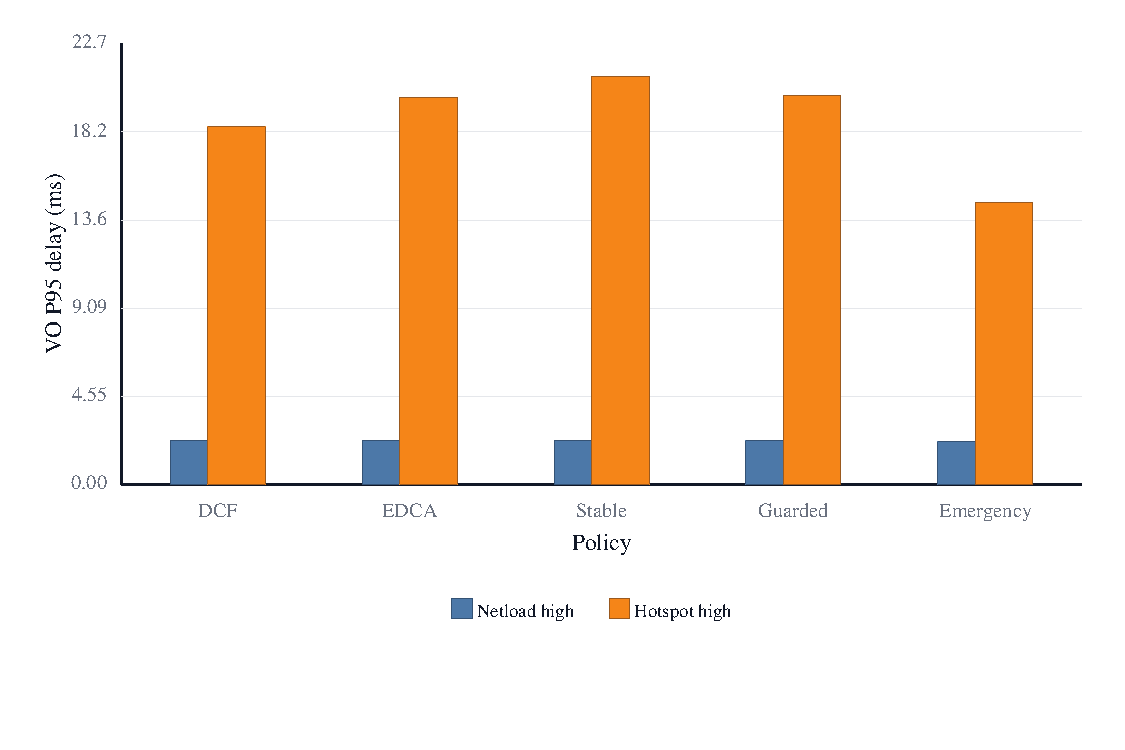
\includegraphics[width=0.95\linewidth, trim=0 50 0 8, clip]{Figs/fig_10_regime_vo_p95_contrast_highway_heavy.pdf}
	\end{center}
	\fonte{Prepared by the author.}
\end{figure}

%%%%%%%%%%%%%%%%%%%%%%%%%%%%%%%%%%%%%%%%%%%%%%%%%%%%%%%%%%%%%%%%%%%%%%%%%%%%%%%%
\section{Hotspot Load: Voice Recovery Under Concentrated Contention}
\label{sec:eval:hotspot}

Under a uniform Poisson offer, near-crash collision opportunities are diffuse across about one hundred senders, so node-local Best Effort suppression removes a negligible share of ambient airtime and can fire only after a first Voice copy was decoded (\autoref{sec:eval:light}).
The enabling contraposition is concentrated airtime: if a few crash-adjacent senders dominate the channel, suppression acquires a target and a Voice effect should appear.

The hotspot overlay \texttt{\_hotspot3} (\autoref{sec:impl:matrix}) implements that regime.
The three vehicles entering the corridor immediately after the crash node bulk-upload about \SI{2.4}{\mega\bit\per\second} each for the whole run, roughly tripling aggregate Best Effort transmissions per run from $22\times10^{3}$ to $72\times10^{3}$.
That higher offer pushes Voice-attributed \gls{mac} losses from about $3.7\times10^{3}$ under uniform \texttt{netload\_high} to about $25\times10^{3}$ under hotspot EDCA \emph{before} policies separate.
The crash source, the alert window, and every metric definition are unchanged; configurations are named \texttt{<policy>\_hotspot\_<profile>}.

\subsection{The \texttt{hotspot\_high} cell}
\label{sec:eval:hotspot:high}

\autoref{tab:eval:hotspot} and \autoref{fig:eval:hotspot_delay} report the dense-burst high-load cell---the only hotspot cell where Voice delay is policy-sensitive.
Plain \gls{dcf} and plain EDCA reach Voice P95 of 18.5--20~ms.
Emergency holds the same tail at 14.6~ms and the Voice mean at 2.78~ms ($-39\%$ mean and $-21\%$ P95 versus plain; $-38\%$ / $-27\%$ versus EDCA).
Voice-attributed collision losses fall from $25.2\times10^{3}$ to $17.8\times10^{3}$ ($-30\%$ versus EDCA), and the three-seed P95 ranges do not overlap the baselines'.
Emergency lowers both central tendency and tail, but P95 remains an order of magnitude above the mean because alert age is dominated by occasional late first-copy successes under collision-heavy windows.
The mechanism is visible in the controller counters: under the 20~ms $\times$~8-copy alert stream the blocked duty cycle is near-continuous---about $16.1\times10^{3}$ Best Effort frames are dropped while blocked (\autoref{tab:eval:hotspot})---so the hot queues never refill the arena during the window.
Multicast reach remains geometry-limited at about ten receivers per alert for every policy: protection buys latency and integrity, not fan-out.

\begin{table}[H]
	\ABNTEXfontereduzida
	\caption{\label{tab:eval:hotspot}Hotspot high-load Voice protection results (100~vehicles, hotspot nodes 1--3 streaming 1200~B, three-run means). \emph{VO \glsentryshort{mac} drops} are Voice-attributed incorrectly-received counts summed over nodes; \emph{\glsentryshort{be} from crash} is the same-sender Best Effort mean delay (starvation under EDCA/\texttt{stable}/\texttt{guarded}); \emph{\glsentryshort{be} dropped blocked} counts emergency preemptions.}
	\begin{center}
		\scriptsize
		\setlength{\tabcolsep}{3.5pt}
		\resizebox{\linewidth}{!}{%
		\begin{tabular}{@{}lrrrrrr@{}}
			\toprule
			\textbf{Policy} &
			\textbf{VO mean (ms)} &
			\textbf{VO P95 (ms)} &
			\textbf{VO RX/alert} &
			\textbf{VO MAC drops ($\times 10^{3}$)} &
			\textbf{\gls{be} from crash (ms)} &
			\textbf{\gls{be} dropped blocked ($\times 10^{3}$)} \\
			\midrule
			Plain     & 4.540 & \shortstack{18.45\\[-1pt]{\scriptsize [16.1--19.9]}} & 9.670 & n.a. & 1.548 & 0 \\
			EDCA      & 4.448 & \shortstack{19.96\\[-1pt]{\scriptsize [18.7--20.7]}} & 9.624 & 25.2 & \shortstack{1453\\[-1pt]{\scriptsize (1.45~s)}} & 0 \\
			Stable    & 4.608 & \shortstack{21.04\\[-1pt]{\scriptsize [18.8--22.8]}} & 9.636 & 25.4 & \shortstack{1386\\[-1pt]{\scriptsize (1.39~s)}} & 0 \\
			Guarded   & 4.439 & \shortstack{20.04\\[-1pt]{\scriptsize [19.8--20.4]}} & 9.689 & 25.1 & \shortstack{981\\[-1pt]{\scriptsize (0.98~s)}} & 0 \\
			Emergency & \textbf{2.781} & \textbf{\shortstack{14.56\\[-1pt]{\scriptsize [11.8--16.0]}}} & \textbf{9.835} & \textbf{17.8} & 3.335 & 16.1 \\
			\bottomrule
		\end{tabular}%
		}
	\end{center}
	\fonte{Prepared by the author.}
\end{table}

\begin{figure}[htb]
	\caption{\label{fig:eval:hotspot_delay}Voice mean and P95 delay by policy at \texttt{hotspot\_high} (100~vehicles). Only emergency, whose preemption keeps hot Best Effort queues out of the collision arena, compresses the tail that hotspot contention inflates.}
	\begin{center}
		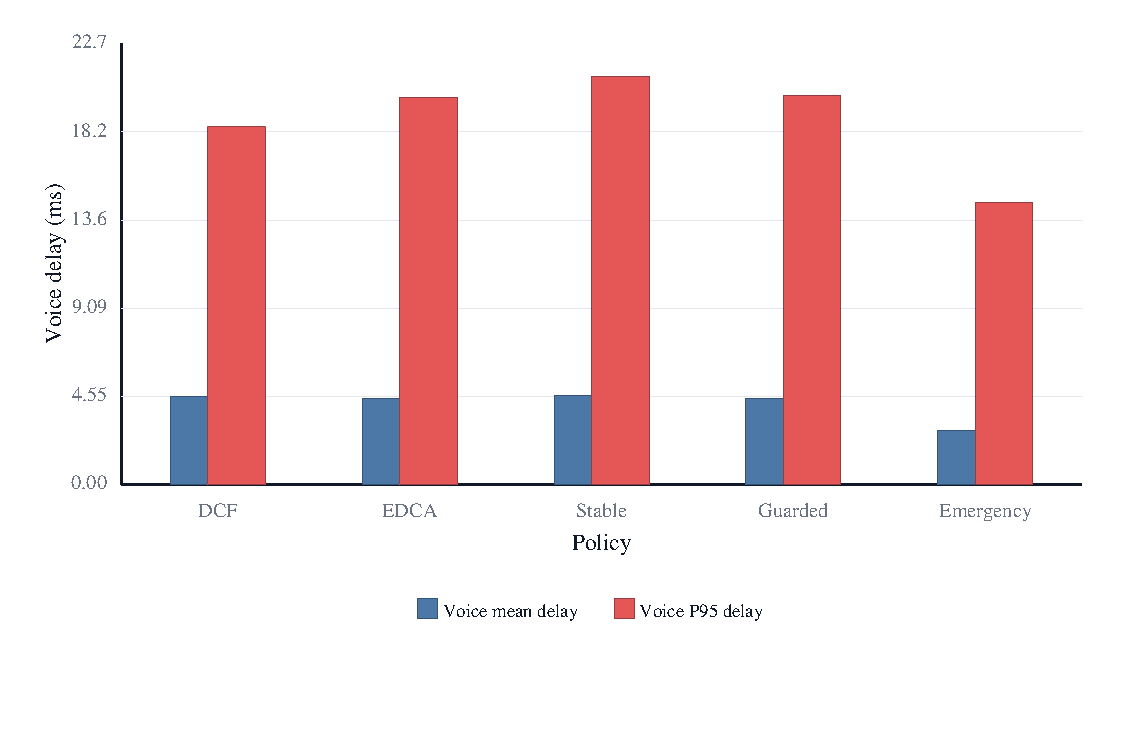
\includegraphics[width=0.95\linewidth, trim=0 50 0 8, clip]{Figs/fig_08_hotspot_vo_delay_by_policy_highway_heavy.pdf}
	\end{center}
	\fonte{Prepared by the author.}
\end{figure}

Dropping, not deferring, is the load-shedding step that matters under concentrated contention.
\texttt{stable} and \texttt{guarded} keep Voice P95 on the EDCA baseline (20--21~ms): blocking without dropping never clears the hot queues.
The same policies starve the crash node's own Best Effort stream---delivered packets from that sender average $0.98$--$1.45$~\si{\second} of queueing delay---whereas emergency and plain keep that same-sender slice at 3.3~ms and 1.5~ms respectively (\autoref{tab:eval:hotspot}).
Preemption therefore doubles as a starvation cure for the alerted node: it is what both recovers Voice and keeps the sender's ordinary traffic responsive when continuous hotspot demand would otherwise own the local arbitration forever.

\subsection{Dose response: why only dense bursts win}
\label{sec:eval:hotspot:dose}

The Voice gain is conditional on burst density (\autoref{tab:eval:hotspot_dose}, \autoref{fig:eval:hotspot_dose}).
At \texttt{hotspot\_high} the 20~ms period with eight copies keeps protection armed for most of the crash window.
At \texttt{medium} (75~ms, four copies) and \texttt{low} (120~ms, three copies) the blocked duty cycle falls to roughly one third or less, hot traffic refills the gaps between blocks, and emergency becomes neutral-to-harmful on the Voice mean ($+10\%$ and $+16\%$ respectively).
Voice service therefore appears only when \emph{both} enabling conditions hold: concentrated near-crash airtime \emph{and} a cadence dense enough to cover it.

\begin{table}[htb]
	\ABNTEXfontereduzida
	\caption{\label{tab:eval:hotspot_dose}Dose response of emergency against plain under hotspot load (three-run means). Voice gains appear only where the burst cadence keeps protection armed for most of the crash window.}
	\begin{center}
		\small
		\setlength{\tabcolsep}{5pt}
		\begin{tabular}{@{}llrr@{}}
			\toprule
			\textbf{Load} & \textbf{Burst profile} & \textbf{$\Delta$ VO mean} & \textbf{$\Delta$ VO P95} \\
			\midrule
			\texttt{high}   & 20~ms $\times$ 8 copies & $-39\%$ & $-21\%$ \\
			\texttt{medium} & 75~ms $\times$ 4 copies & $+10\%$ & $+5\%$ \\
			\texttt{low}    & 120~ms $\times$ 3 copies & $+16\%$ & $+0\%$ \\
			\bottomrule
		\end{tabular}
	\end{center}
	\fonte{Prepared by the author.}
\end{table}

\begin{figure}[htb]
	\caption{\label{fig:eval:hotspot_dose}Voice P95 delay across offered-load profiles under hotspot load (100~vehicles), plain versus emergency (three-seed means). Protection differentiates only at \texttt{high}, where dense bursts keep Best Effort suppression armed for most of the crash window.}
	\begin{center}
		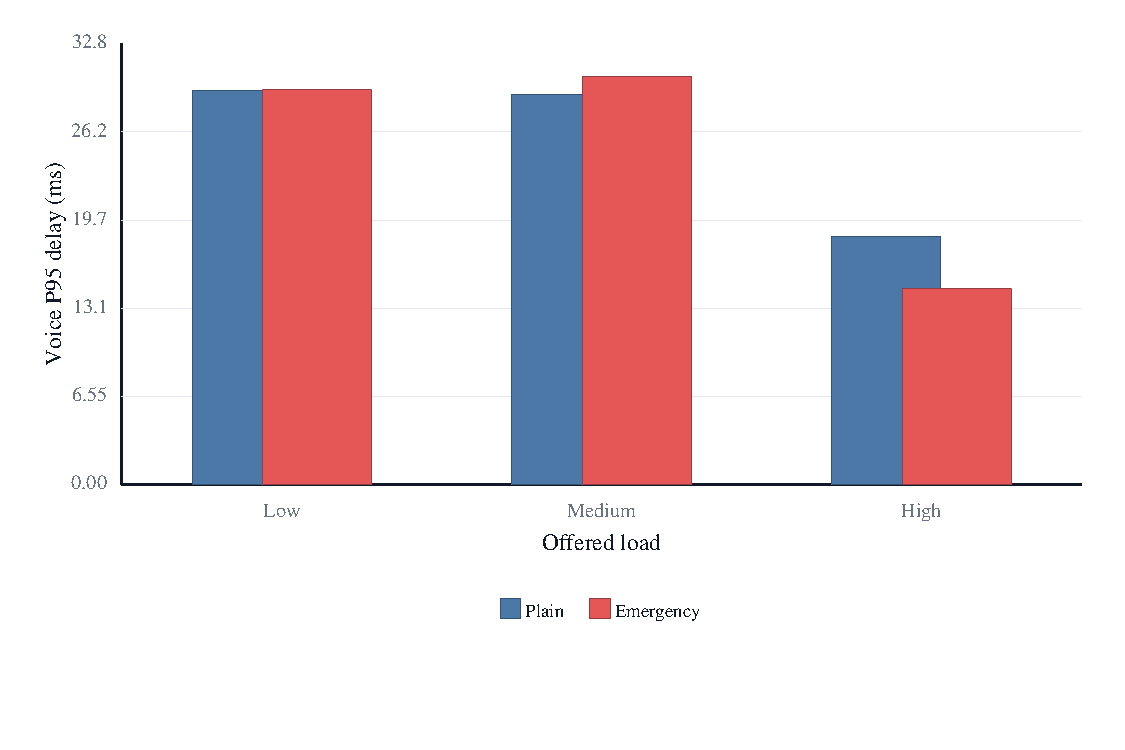
\includegraphics[width=0.95\linewidth, trim=0 50 0 8, clip]{Figs/fig_09_hotspot_vo_p95_by_load_highway_heavy.pdf}
	\end{center}
	\fonte{Prepared by the author.}
\end{figure}

%%%%%%%%%%%%%%%%%%%%%%%%%%%%%%%%%%%%%%%%%%%%%%%%%%%%%%%%%%%%%%%%%%%%%%%%%%%%%%%%
\section{Uniform Load: The Null Voice Case}
\label{sec:eval:light}

The uniform Poisson matrix is the scientific null against which \autoref{sec:eval:hotspot} is read.
With no concentrated near-crash sender, every policy keeps Voice alert age within a few tens of microseconds of plain \gls{dcf}; the policy contrast is Best Effort cost.

\subsection{Light-density gating numbers}
\label{sec:eval:light:gating}

\autoref{tab:eval:light} reports light-density high-load cells versus \texttt{plain\_netload\_high}.
Voice stays flat near 2.08~ms P95 (within $1.3\%$ of plain).
\texttt{stable} and \texttt{guarded} inflate Best Effort P95 from 0.44~ms to 49~ms and 9.0~ms; emergency shortens it to 0.37~ms by dropping stale Best Effort work rather than by protecting Voice.
The sweep is a gating test: adaptive blocking without dropping is already risky when protection windows can open under low channel stress.

\begin{table}[htb]
	\ABNTEXfontereduzida
	\caption{\label{tab:eval:light}Light-density high-load gating results versus \texttt{plain\_netload\_high} (10~vehicles, three-seed means). Voice columns are relative changes; Best Effort P95 is absolute (ms) so four-digit percentages do not dominate the table. Plain baselines (ms): Voice mean 0.786, Voice P95 2.078, Best Effort mean 0.383, Best Effort P95 0.437.}
	\begin{center}
		\setlength{\tabcolsep}{5pt}
		\begin{tabular}{@{}lrrr@{}}
			\toprule
			\textbf{Policy} &
			\textbf{VO mean} &
			\textbf{VO P95} &
			\textbf{BE P95 (ms)} \\
			\midrule
			Plain (baseline) & --- & --- & 0.44 \\
			EDCA      & $+1.3\%$  & $-0.0\%$   & 0.42 \\
			Stable    & $+0.9\%$  & $+0.5\%$  & 49 \\
			Guarded   & $-1.3\%$  & $-1.3\%$  & 9.0 \\
			Emergency & $+2.4\%$ & $+0.2\%$ & 0.37 \\
			\bottomrule
		\end{tabular}
	\end{center}
	\fonte{Prepared by the author.}
\end{table}

\subsection{Heavy-density confirmation}
\label{sec:eval:heavy:qos}

At one hundred vehicles the same null Voice story holds, only louder.
\autoref{tab:eval:heavy_qos} and \autoref{fig:eval:p95_gap_heavy} show Voice mean, P95, and jitter within a few tens of microseconds across all five policies (P95 2.21--2.25~ms).
EDCA does not lower Voice alert age relative to plain \gls{dcf}.
The policy contrast is Best Effort: \texttt{stable} raises fleet Best Effort P95 from 0.51~ms to 30~ms; \texttt{guarded} to 3.9~ms; emergency keeps 0.37~ms by preemption.
That lower emergency P95 is not better Best Effort service: delay is measured only on delivered packets, so dropping frames while blocked removes the slow tail from the sample while the cost appears as reach loss (Best Effort RX/TX falls from 8.06 under \texttt{plain} to 6.93).
Voice RX/alert is 9.95 for every policy (geometry-limited fan-out).
Voice-attributed \gls{mac} drops sit near $3.7\times10^{3}$ under every QoS-enabled policy and do not separate emergency from EDCA; Best Effort queue overflow is zero throughout.
Node-local suppression therefore has no Voice target under diffuse contention: it cannot change how many alerts arrive or how many collide.

\begin{table}[htb]
	\ABNTEXfontereduzida
	\caption{\label{tab:eval:heavy_qos}Heavy-density high-load delay, jitter, and multicast reach (100~vehicles, three-run means with min--max range across seeds; delays and jitter in~ms).}
	\begin{center}
		\small
		\setlength{\tabcolsep}{6pt}
		\begin{tabular}{@{}lrrrr@{}}
			\toprule
			\multicolumn{5}{@{}l}{\textit{\gls{vo} (crash alert)}} \\
			\midrule
			\textbf{Policy} & \textbf{Mean} & \textbf{P95} & \textbf{Jitter} & \textbf{RX/alert} \\
			\midrule
			Plain      & \shortstack{0.991\\[-1pt]{\scriptsize [0.975--1.021]}} & \shortstack{2.249\\[-1pt]{\scriptsize [2.229--2.287]}} & \shortstack{1.024\\[-1pt]{\scriptsize [1.010--1.044]}} & \shortstack{9.954\\[-1pt]{\scriptsize [8.743--10.843]}} \\
			EDCA       & \shortstack{0.994\\[-1pt]{\scriptsize [0.982--1.003]}} & \shortstack{2.242\\[-1pt]{\scriptsize [2.220--2.255]}} & \shortstack{1.018\\[-1pt]{\scriptsize [1.005--1.034]}} & \shortstack{9.954\\[-1pt]{\scriptsize [8.743--10.843]}} \\
			Stable     & \shortstack{0.988\\[-1pt]{\scriptsize [0.958--1.026]}} & \shortstack{2.245\\[-1pt]{\scriptsize [2.238--2.255]}} & \shortstack{1.026\\[-1pt]{\scriptsize [0.995--1.057]}} & \shortstack{9.954\\[-1pt]{\scriptsize [8.743--10.843]}} \\
			Guarded    & \shortstack{0.998\\[-1pt]{\scriptsize [0.991--1.004]}} & \shortstack{2.241\\[-1pt]{\scriptsize [2.225--2.253]}} & \shortstack{1.029\\[-1pt]{\scriptsize [1.013--1.042]}} & \shortstack{9.954\\[-1pt]{\scriptsize [8.743--10.843]}} \\
			Emergency  & \shortstack{0.952\\[-1pt]{\scriptsize [0.948--0.960]}} & \shortstack{2.211\\[-1pt]{\scriptsize [2.203--2.226]}} & \shortstack{0.979\\[-1pt]{\scriptsize [0.955--1.007]}} & \shortstack{9.954\\[-1pt]{\scriptsize [8.743--10.843]}} \\
			\midrule
			\multicolumn{5}{@{}l}{\textit{\gls{be} (background)}} \\
			\midrule
			\textbf{Policy} & \textbf{Mean} & \textbf{P95} & \textbf{Jitter} & \textbf{RX/TX} \\
			\midrule
			Plain      & \shortstack{0.387\\[-1pt]{\scriptsize [0.387--0.388]}} & \shortstack{0.511\\[-1pt]{\scriptsize [0.509--0.513]}} & \shortstack{0.035\\[-1pt]{\scriptsize [0.034--0.035]}} & \shortstack{8.057\\[-1pt]{\scriptsize [7.617--8.321]}} \\
			EDCA       & \shortstack{0.389\\[-1pt]{\scriptsize [0.388--0.390]}} & \shortstack{0.524\\[-1pt]{\scriptsize [0.507--0.538]}} & \shortstack{0.038\\[-1pt]{\scriptsize [0.036--0.040]}} & \shortstack{8.091\\[-1pt]{\scriptsize [7.687--8.363]}} \\
			Stable     & \shortstack{3.696\\[-1pt]{\scriptsize [3.560--3.944]}} & \shortstack{30.491\\[-1pt]{\scriptsize [27.614--34.175]}} & \shortstack{3.490\\[-1pt]{\scriptsize [3.374--3.598]}} & \shortstack{7.606\\[-1pt]{\scriptsize [7.295--7.777]}} \\
			Guarded    & \shortstack{0.896\\[-1pt]{\scriptsize [0.801--0.951]}} & \shortstack{3.889\\[-1pt]{\scriptsize [2.955--4.458]}} & \shortstack{0.669\\[-1pt]{\scriptsize [0.569--0.720]}} & \shortstack{7.655\\[-1pt]{\scriptsize [7.319--7.848]}} \\
			Emergency  & \shortstack{0.432\\[-1pt]{\scriptsize [0.413--0.461]}} & \shortstack{\textbf{0.369}\\[-1pt]{\scriptsize [0.369--0.369]}} & \shortstack{0.120\\[-1pt]{\scriptsize [0.086--0.172]}} & \shortstack{6.927\\[-1pt]{\scriptsize [6.692--7.046]}} \\
			\bottomrule
		\end{tabular}
	\end{center}
	\fonte{Prepared by the author.}
\end{table}

\begin{figure}[htb]
	\caption{\label{fig:eval:p95_gap_heavy}Voice and Best Effort P95 delay at \texttt{netload\_high}, heavy density (100~vehicles), dual panel. Top: Voice alert age stays near 2.2~ms for every policy. Bottom: \texttt{stable} stretches fleet Best Effort P95 to 30~ms while emergency keeps it at 0.37~ms by dropping competing frames. The horizontal axis, labelled \emph{Strategy} here, carries the same five policies as the \emph{Policy} axis of \autoref{fig:eval:regime_contrast}.}
	\begin{center}
		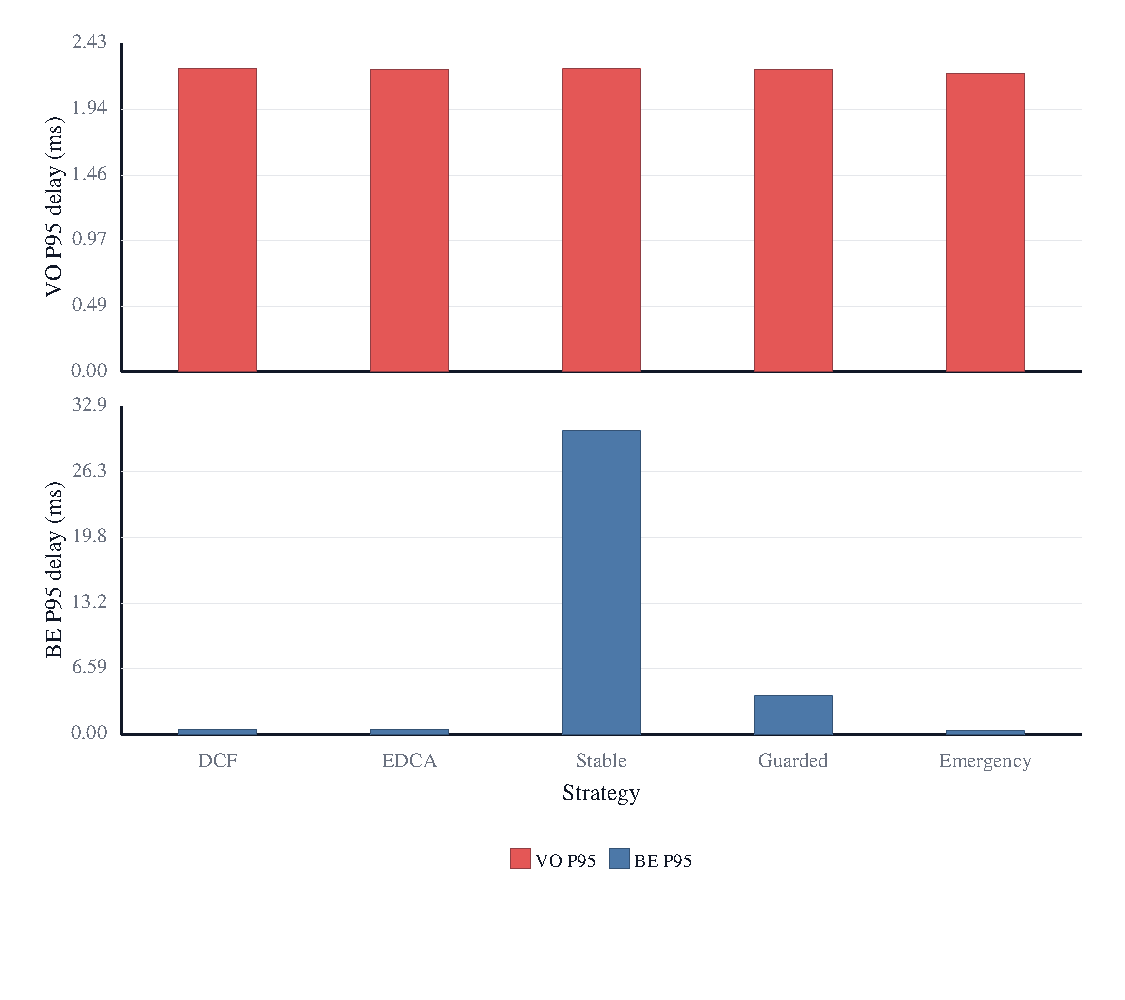
\includegraphics[width=0.92\linewidth, trim=0 50 0 8, clip]{Figs/fig_01_p95_delay_priority_gap_highway_heavy.pdf}
	\end{center}
	\fonte{Prepared by the author.}
\end{figure}

The floor that every policy shares is set by the alert generator itself rather than by channel access.
Each physical copy of a burst---including the first---is dispatched at an offset $\max(0,\,U(-J,\,J))$ after the logical burst timestamp that defines the delay origin, where $J$ is the configured repeat jitter (\autoref{sec:impl:crash}).
That offset therefore has a point mass at zero and a 95th percentile of $0.9\,J$: about \SI{1.8}{\milli\second} at the high-load setting $J=\SI{2}{\milli\second}$ and about \SI{4.5}{\milli\second} at the low and medium setting $J=\SI{5}{\milli\second}$.
Adding the sub-millisecond transfer delay measured on the same samples reproduces the observed floors of about 2.2~ms and 4.6--4.9~ms respectively, and the mean behaves the same way: $\E[\max(0,\,U(-2,2))]=\SI{0.5}{\milli\second}$ accounts for half of the 0.99~ms Voice mean in \autoref{tab:eval:heavy_qos}.
Only when the first copy is lost does the inter-copy gap~$g$ enter, adding one further quantum per missed repeat---the application-level repetition on which robust vehicular broadcast schemes rely~\cite{Robust_Broadcast_Ma,Reliable_Broadcast_Farnoud}.
At the 95th percentile under diffuse load that regime is rare, so contention shifts probability mass within a generator-imposed floor instead of creating a \gls{mac}-policy lever.
Two consequences follow for how the 2.2~ms figure should be read: it is not a pure medium-access measurement, and no MAC policy could have moved it.

%%%%%%%%%%%%%%%%%%%%%%%%%%%%%%%%%%%%%%%%%%%%%%%%%%%%%%%%%%%%%%%%%%%%%%%%%%%%%%%%
\section{The Best Effort Cost of Protection}
\label{sec:eval:cost}

Section~\ref{sec:eval:hotspot} established what emergency preemption \emph{buys} under concentrated load.
This section prices what protection \emph{costs}, starting from the hotspot cell and then noting the same mechanism under uniform load---where there is no Voice return.

\subsection{Hotspot pricing}
\label{sec:eval:cost:hotspot}

At \texttt{hotspot\_high} the Best Effort bill is inseparable from the Voice win.
Emergency drops about $16.1\times10^{3}$ Best Effort frames while blocked (\autoref{tab:eval:hotspot}).
That preemption is also what prevents crash-node Best Effort starvation: under EDCA/\texttt{stable}/\texttt{guarded} the same-sender Best Effort mean reaches $0.98$--$1.45$~\si{\second}, versus 3.3~ms under emergency.
\autoref{fig:eval:gain_cost} places the tradeoff in $\Delta$-space versus plain \gls{dcf}: under hotspot high load, emergency alone moves left on the Voice axis; under uniform high load the adaptive policies buy no Voice P95 reduction while Best Effort P95 rises---especially under \texttt{stable}.

\begin{figure}[htb]
	\caption{\label{fig:eval:gain_cost}Voice-gain versus Best Effort cost relative to plain \glsentryshort{dcf} at high load (three-seed means). Dual panels use independent axes: left is uniform \texttt{netload\_high}; right is \texttt{hotspot\_high}. Negative $\Delta$ Voice P95 is an improvement; positive $\Delta$ Best Effort P95 is a penalty.}
	\begin{center}
		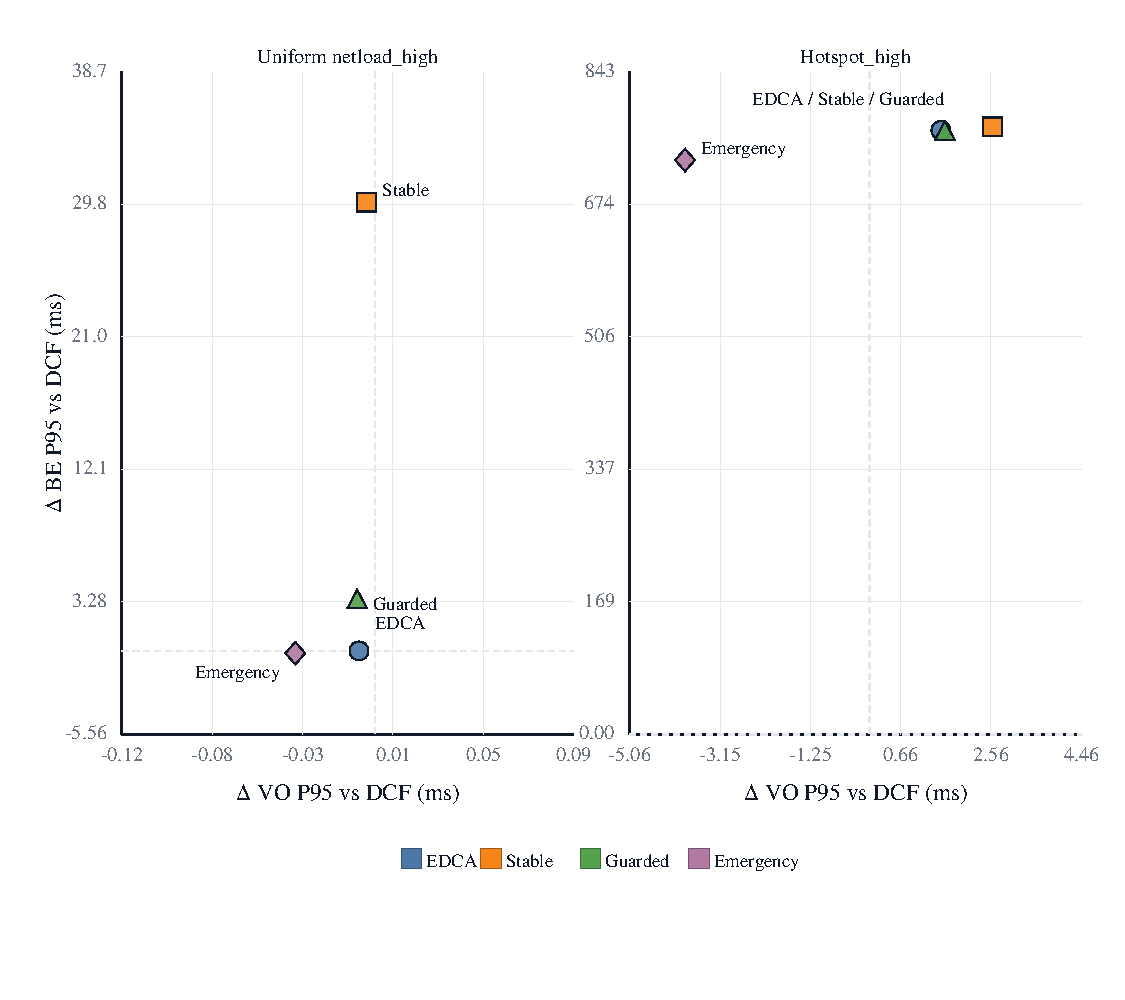
\includegraphics[width=0.95\linewidth, trim=0 50 0 8, clip]{Figs/fig_04_vo_gain_vs_be_cost_highway_heavy.pdf}
	\end{center}
	\fonte{Prepared by the author.}
\end{figure}

\subsection{Uniform-load cost without a Voice target}
\label{sec:eval:heavy:ladder}

Under the uniform matrix the same controller still fires, but without a Voice return (\autoref{tab:eval:heavy_p95}, \autoref{tab:eval:heavy_ctrl}, \autoref{fig:eval:ctrl}).
\texttt{stable} and \texttt{guarded} accumulate about $1.1\times10^{5}$ protection activations per high-load run with zero preemption counters, stretching fleet Best Effort P95 to 30~ms and 3.9~ms.
Emergency pays about $2.5\times10^{3}$ Best Effort drops while blocked plus twelve suppressed grants and keeps fleet and crash-sender tails at 0.37~ms and 0.44~ms---below plain---while Voice P95 remains on the 2.2~ms floor.
In short: deferral buys delay; dropping buys silence; only dropping yields Voice service once a concentrated target exists (\autoref{sec:eval:hotspot}).

\begin{table}[htb]
	\ABNTEXfontereduzida
	\caption{\label{tab:eval:heavy_p95}Best Effort 95th-percentile delay (ms) across offered-load regimes for the five-policy ladder (100~vehicles, three-run means with min--max range across seeds). Voice rows are omitted: Voice P95 stays on the generator's dispatch-jitter floor for every policy (\autoref{sec:eval:light}). Cells with a vanishing seed spread omit the range.}
	\begin{center}
		\scriptsize
		\setlength{\tabcolsep}{3pt}
		\begin{tabularx}{\linewidth}{@{}l *{5}{>{\centering\arraybackslash}X}@{}}
			\toprule
			\textbf{Load} & \textbf{Plain} & \textbf{EDCA} & \textbf{Stable} & \textbf{Guarded} & \textbf{Emerg.} \\
			\midrule
			\multicolumn{6}{@{}l}{\textit{\gls{be} (background, fleet)}} \\
			\texttt{low}    & 0.217 & 0.217 & \shortstack{0.323\\[-1pt]{\scriptsize [0.217--0.419]}} & 0.217 & 0.217 \\
			\texttt{medium} & 0.297 & 0.297 & \shortstack{2.081\\[-1pt]{\scriptsize [0.711--3.203]}} & \shortstack{0.357\\[-1pt]{\scriptsize [0.297--0.387]}} & 0.297 \\
			\texttt{high}   & \shortstack{0.511\\[-1pt]{\scriptsize [0.509--0.513]}} & \shortstack{0.524\\[-1pt]{\scriptsize [0.507--0.538]}} & \shortstack{30.491\\[-1pt]{\scriptsize [27.614--34.175]}} & \shortstack{3.889\\[-1pt]{\scriptsize [2.955--4.458]}} & \textbf{0.369} \\
			\addlinespace
			\multicolumn{6}{@{}l}{\textit{\gls{be} from the crash node}} \\
			\texttt{low}    & 0.217 & 0.217 & \shortstack{0.708\\[-1pt]{\scriptsize [0.641--0.753]}} & \shortstack{1.357\\[-1pt]{\scriptsize [0.217--2.871]}} & 0.217 \\
			\texttt{medium} & 0.297 & \shortstack{0.335\\[-1pt]{\scriptsize [0.297--0.411]}} & \shortstack{3.040\\[-1pt]{\scriptsize [2.419--3.814]}} & \shortstack{2.323\\[-1pt]{\scriptsize [1.197--3.110]}} & 0.297 \\
			\texttt{high}   & \shortstack{0.631\\[-1pt]{\scriptsize [0.621--0.651]}} & \shortstack{0.772\\[-1pt]{\scriptsize [0.731--0.842]}} & \shortstack{13.763\\[-1pt]{\scriptsize [13.541--13.955]}} & \shortstack{3.865\\[-1pt]{\scriptsize [3.769--3.944]}} & \shortstack{\textbf{0.435}\\[-1pt]{\scriptsize [0.369--0.567]}} \\
			\bottomrule
		\end{tabularx}
	\end{center}
	\fonte{Prepared by the author.}
\end{table}

\begin{table}[H]
	\ABNTEXfontereduzida
	\caption{\label{tab:eval:heavy_ctrl}Adaptive-controller actions at heavy-density high load (three-run means; Voice-protection and Best Effort-drop columns in thousands, $\times 10^{3}$; Best Effort hold is a raw event count). The \texttt{emergency} hold entry is about 12 grant-suppression events.}
	\begin{center}
		\small
		\setlength{\tabcolsep}{5pt}
		\begin{tabular}{@{}lrrr@{}}
			\toprule
			\textbf{Policy} &
			\textbf{VO protection} &
			\textbf{BE drop while blocked} &
			\textbf{BE hold} \\
			\midrule
			Stable    & 115  & 0  & 0 \\
			Guarded   & 115  & 0  & 0 \\
			Emergency & 127 & 2.53 & 12 \\
			\bottomrule
		\end{tabular}
	\end{center}
	\fonte{Prepared by the author.}
\end{table}

\begin{figure}[htb]
	\caption{\label{fig:eval:ctrl}Adaptive-controller actions by offered load, heavy density (three panels): Voice-protection activations, Best Effort grants suppressed while blocked, and Best Effort frames dropped while blocked. Emergency alone combines protection with explicit preemption; \texttt{stable} and \texttt{guarded} mainly accumulate protection windows without dropping.}
	\begin{center}
		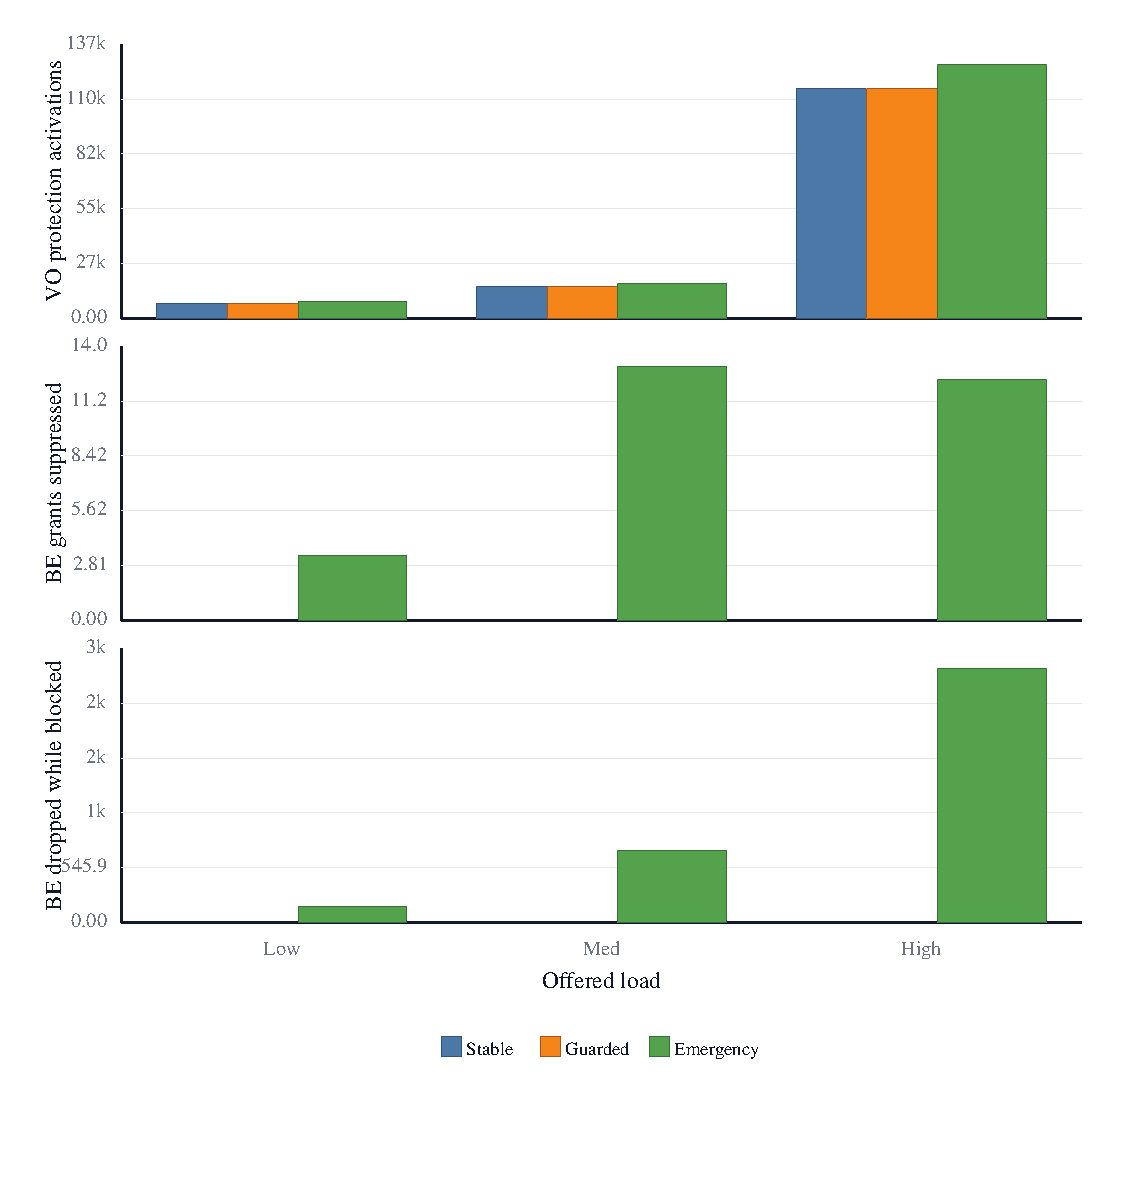
\includegraphics[width=0.88\linewidth, trim=0 50 0 8, clip]{Figs/fig_07_v2x_control_actions_by_load_highway_heavy.pdf}
	\end{center}
	\fonte{Prepared by the author.}
\end{figure}

\section{Discussion}
\label{sec:eval:discussion}

\subsection{Event-triggered escalation, not always-on QoS}
\label{sec:eval:disc:escalation}

Adaptive blocking is harmful when armed without Voice-limited congestion: \texttt{stable} and \texttt{guarded} inflate Best Effort delay while Voice alert age stays put (\autoref{sec:eval:light}).
The mechanism should be treated as an escalation level attached to genuine channel stress, not as an always-on replacement for ordinary EDCA marking~\cite{IEEE80211e_2005,aguiar2026_veins_qos}.
Explicit DSCP-to-Voice mapping remains a reasonable default; bounded or emergency suppression should be reserved for the concentrated regime of \autoref{sec:eval:hotspot}, where preemption flips from pure cost to measured Voice benefit (\autoref{tab:eval:hotspot}).

\subsection{Reading the baseline correctly}
\label{sec:eval:disc:plain}

Two measurement traps are aggregation artifacts rather than policy effects.
First, under \texttt{plain} both classes receive identical per-frame \gls{mac} treatment, yet \autoref{tab:eval:heavy_qos} shows a Voice--Best Effort delay gap: the gap reflects different traffic processes (one crash-node alert stream versus a fleet-wide Poisson offer), not a differentiating \gls{dcf} queue.
Second, Voice RX/alert exceeds Best Effort RX/TX for structural reasons---different denominators and a denser neighborhood around the stopped crash node.
Cross-class comparisons within one policy therefore describe different traffic processes; the crash-node Best Effort slice is the controlled same-sender check, and cross-policy comparisons within one class remain the policy measurement.
Poisson redraws keep Best Effort offer at about 22~thousand transmissions on every uniform run, so seeds no longer split into an uncongested draw and two saturated draws.

\subsection{Regime-conditional significance of the Voice effects}
\label{sec:eval:disc:significance}

Under the uniform matrix there is no Voice-tail reduction to claim against representative V2X latency budgets such as the~\SI{25}{\milli\second} end-to-end bound for cooperative platooning in \gls{threegpp} TS~22.186~\cite{ts22186}: absolute Voice P95 stays near 2.2~ms for every policy (\autoref{sec:eval:light}).
That margin is moreover partly structural rather than earned by the channel, since about \SI{1.8}{\milli\second} of the 2.2~ms is the alert generator's own per-copy dispatch jitter (\autoref{sec:eval:light}); the medium-access contribution to the uniform-load tail is smaller still.
The hotspot cell of \autoref{tab:eval:hotspot} is where absolute tails re-enter that budget band and where emergency compresses them.
Three seeds per cell keep this a mechanism check rather than an effect-size estimate (\autoref{sec:eval:disc:limits}); the boundary itself is the take-home---the same preemption is a cost center under uniform load and a Voice lever under concentrated load.

\subsection{Protection cost, class granularity, and spatial fairness}
\label{sec:eval:disc:cost}

Bounded protection makes Best Effort service worse than plain \gls{dcf} at high uniform load, and emergency converts part of the backlog into explicit loss while keeping the fleet Best Effort tail short (\autoref{sec:eval:cost}).
Because the model treats \emph{all} Best Effort traffic as suppressible, these penalties are a worst-case bound for the two-class abstraction (\autoref{sec:sys:scope}): in a real stack, traffic outside the current crash alert may still be safety relevant.
Deployments would need finer-grained classes before comparable \gls{mac} aggression, and the trade-off is defensible only for genuinely critical, short-lived flows such as the alert window studied here.

\label{sec:eval:disc:spatial}
Nor is the penalty uniform across vehicles: protection is armed locally by overheard Voice frames, so vehicles near the crash source defer or drop Best Effort while distant vehicles continue unaffected (\autoref{sec:sys:controller}).
The Best Effort cost is spatially concentrated around the event---arguably desirable for a crash---but pooled averages understate the worst-affected vehicles; per-vehicle fairness is left as future work.

\subsection{Preemption as a starvation cure under concentrated contention}
\label{sec:eval:disc:starvation}

Under concentrated contention, \gls{edca}-family queues can starve the very node they should serve first.
At \texttt{hotspot\_high}, crash-node Best Effort means of $0.98$--$1.45$~\si{\second} under EDCA/\texttt{stable}/\texttt{guarded} collapse to 3.3~ms under emergency (\autoref{tab:eval:hotspot}).
Dropping is therefore both the Voice lever and the starvation cure when continuous hotspot demand would otherwise own local arbitration.

\subsection{Burst cadence as an online arming trigger}
\label{sec:eval:disc:trigger}

The dose-response of \autoref{tab:eval:hotspot_dose} implies a measurable online signal for deciding when protection is worth its cost: arm emergency suppression only while recent alert cadence times the bounded block window (\autoref{tab:impl:parameters}) saturates the available blocking budget.
The controller already tracks activation count and \texttt{maxContinuousBlock}, so the trigger is an instrumentation problem, not a new measurement.
This closes the escalation design loop of \autoref{sec:eval:disc:escalation}.

\subsection{Denial-of-service risk of Voice-triggered suppression}
\label{sec:eval:disc:dos}

Protection is armed by local Voice queue pressure and \emph{overheard} Voice frames without authenticating the sender, so a faulty or malicious node continuously emitting Voice-marked traffic could keep nearby vehicles in blocking mode.
The risk is bounded but not removed: protection windows are finite (20--80~ms maximum continuous block plus a guard interval, \autoref{tab:impl:parameters}) and suppression affects only a node's own Best Effort transmissions.
Real deployment would additionally require V2X message authentication, rate limiting of alert bursts, and plausibility checks before Voice frames may trigger suppression.

\subsection{Limitations and threats to validity}
\label{sec:eval:disc:limits}

Heavy-density \glspl{kpi} average three seeds and report the min--max range on headline delay tables, still without confidence intervals or significance tests, so results are qualitative mechanism checks rather than proven effect sizes; all observed prioritization is statistical contention shaping, not deterministic real-time communication~\cite{kosekszott2012What}.
The evaluation is simulation-only, models a single crash source on a one-hop highway corridor, and uses the simplified \gls{phy} assumptions of \autoref{chap:implementation} and \autoref{sec:sys:scope}; concurrent alerts would arm overlapping protection windows whose interaction is not evaluated.
Results do not predict absolute performance under richer propagation or congestion control, and no adaptive-EDCA or \gls{dcc} baseline is implemented, so no superiority claim is made against those families~\cite{etsi_dcc_2018}.
The configured \gls{edca} parameters follow the IEEE~802.11 BSS QoS defaults rather than the distinct \gls{ocb} default set, and group-addressed frames use \gls{inet}'s default fastest-mandatory-mode rate selection rather than a basic-rate policy (\autoref{sec:impl:radio}); both choices are uniform across policies but may shift absolute values relative to deployed 802.11p stacks.
The \texttt{high} crash-burst profile is a deliberate stress case rather than a standardized alert schedule, and no application-level safety deadline is evaluated.
The three adaptive profiles are fixed design points whose triggers are not individually ablated, although their spread of block windows (4--15~ms) and Voice thresholds (1--3 packets) acts as a coarse sensitivity ladder; a systematic parameter sweep is future work.
The hotspot cells place streaming nodes by injection order rather than by a received-power map, so the exact gain magnitudes depend on that geometry; the sign of the effect---and its absence at sparser burst cadences---is the claim, not the decimals.
Within that scope the comparison remains internally fair: all configurations share the same \gls{phy} stack, mobility trace, and load matrix, isolating \gls{mac}-policy effects~\cite{aguiar2026_veins_qos}.

%%%%%%%%%%%%%%%%%%%%%%%%%%%%%%%%%%%%%%%%%%%%%%%%%%%%%%%%%%%%%%%%%%%%%%%%%%%%%%%%
\section{Chapter Summary}
\label{sec:eval:summary}

The evaluation compared five \gls{mac} policies on the same highway matrix and found a regime-conditional answer rather than a universal Voice-tail race.
The primary positive result is \texttt{hotspot\_high}: emergency preemption recovers Voice service when near-crash airtime is concentrated and bursts are dense enough to keep protection armed (\autoref{tab:eval:hotspot}).
The uniform Poisson matrix is the null that makes that result conditional: Voice alert age stays on the generator's dispatch-jitter floor for every policy, while adaptive blocking mainly taxes Best Effort (\autoref{sec:eval:light}).
Bounded blocking without dropping (\texttt{stable}, \texttt{guarded}) never converts hotspot stress into Voice service; dropping is the load-shedding step that both compresses the Voice tail and cures crash-node Best Effort starvation.
The practical takeaway is therefore conditional: explicit DSCP-to-Voice marking is a reasonable default; adaptive blocking---especially emergency preemption---is justified as an event-triggered escalation where near-crash congestion is concentrated, with authentication and rate limiting as deployment prerequisites.

The subsequent chapter concludes the dissertation by summarizing these findings, stating the conditional practical takeaway, and outlining limitations and future work.


% ---
% 6 - Conclusion
% ---
\chapter{Conclusion}
\label{chap:conclusion}

This dissertation asked whether crash-triggered Voice traffic can obtain better wireless service than ordinary Best Effort under contention in decentralized vehicular Wi-Fi, and at what cost that protection is paid.
The answer was pursued with a deliberately minimal two-class model: all vehicles exchange periodic Best Effort multicast, one designated crash source injects temporary Voice alert bursts marked DSCP~46, and five \gls{mac} policies are compared on the same highway matrix---plain \gls{dcf}, EDCA with explicit Voice mapping, and three adaptive extensions (\texttt{stable}, \texttt{guarded}, \texttt{emergency}) that suppress competing Best Effort while alerts are active~(\autoref{chap:sysmodel}, \autoref{chap:implementation}).
The evaluation is simulation-only and mechanism-oriented: it isolates statistical contention shaping under controlled load and density, not deterministic real-time guarantees or application-level crash outcomes~(\autoref{chap:evaluation})~\cite{kosekszott2012What,IEEE80211e_2005,aguiar2026_veins_qos}.

%%%%%%%%%%%%%%%%%%%%%%%%%%%%%%%%%%%%%%%%%%%%%%%%%%%%%%%%%%%%%%%%%%%%%%%%%%%%%%%%
\section{Main Findings}
\label{sec:conc:findings}

Under heavy density and high offered load, Voice 95th-percentile alert age is about 2.2~ms under every policy: EDCA does not beat plain \gls{dcf}, and emergency's 2.21~ms versus 2.24~ms is not a material Voice-tail win.
The policy contrast is Best Effort cost.
\texttt{stable} raises fleet Best Effort P95 from 0.51~ms under plain \gls{dcf} to 30~ms; \texttt{guarded} to 3.9~ms; emergency keeps 0.37~ms by dropping competing frames (about $2.5\times10^{3}$ Best Effort drops while blocked)~\cite{aguiar2026_veins_qos}.

The light-density high-load sweep is the same gating test rather than a Voice-gain story.
Bounded adaptive profiles (\texttt{stable}/\texttt{guarded}) leave Voice P95 at 2.08~ms while inflating Best Effort P95 to 49~ms and 9.0~ms; only emergency shortens the Best Effort tail, by preemption rather than by protecting Voice.
Cross-reading both densities shows an enabling condition that this matrix does not meet: adaptive blocking would help Voice only when removing Best Effort competition actually shortens alert service; under a Poisson 125~ms offer it mainly shifts delay onto ordinary traffic.

%%%%%%%%%%%%%%%%%%%%%%%%%%%%%%%%%%%%%%%%%%%%%%%%%%%%%%%%%%%%%%%%%%%%%%%%%%%%%%%%
\section{Practical Takeaway}
\label{sec:conc:takeaway}

The practical takeaway is therefore conditional.
Explicit DSCP-to-Voice mapping remains a reasonable default for crash-marked alerts~\cite{IEEE80211e_2005}.
Adaptive Best Effort suppression---especially emergency preemption---should be treated as an event-triggered escalation level attached to genuine congestion and genuine alert activity, not as an always-on replacement for ordinary EDCA.
Deployment would additionally require authentication, rate limiting, and plausibility checks before overheard Voice frames may arm suppression, because the same local trigger that protects a crash can be abused by faulty or malicious Voice traffic (\autoref{chap:evaluation}).

The absolute Voice delays in this synthetic setting remain far below representative platooning latency budgets such as the~\SI{25}{\milli\second} end-to-end bound in \gls{threegpp} TS~22.186~\cite{ts22186}.
The contribution is accordingly \gls{mac}-level cost accounting under a Poisson offer, not a claim that the simulated scenario already improves crash outcomes at the application layer.

%%%%%%%%%%%%%%%%%%%%%%%%%%%%%%%%%%%%%%%%%%%%%%%%%%%%%%%%%%%%%%%%%%%%%%%%%%%%%%%%
\section{Limitations}
\label{sec:conc:limits}

The study's limits are those already argued in the Evaluation discussion (\autoref{sec:eval:discussion}); they are restated here as the boundary conditions on the Conclusion.

\noindent\textbf{Simulation scope and statistical strength.}
The evaluation is simulation-only, with no testbed or hardware validation, so claims remain tied to the configured Veins/\gls{inet} model~\cite{aguiar2026_veins_qos}.
Heavy-density \glspl{kpi} average three seeds and report the min--max range on headline delay tables, still without confidence intervals or significance tests, and light-density results use the same three-seed rule; the numbers are therefore qualitative mechanism checks under a controlled matrix, not proven effect sizes.
All observed prioritization is statistical contention shaping, not deterministic real-time communication~\cite{kosekszott2012What}.

\medskip
\noindent\textbf{Traffic abstraction and baselines.}
The traffic model is a synthetic two-class Best Effort / Voice abstraction rather than \gls{cam}/\gls{denm} schedules or richer multi-class ITS stacks, and the high crash-burst profile is a deliberate stress case rather than a standardized alert timetable.
Treating \emph{all} Best Effort as suppressible is a worst-case bound for that abstraction: in a real stack, traffic outside the current crash alert may still be safety relevant, so a binary split can underestimate preemption harm (\autoref{sec:eval:disc:cost}).
No adaptive-EDCA or \gls{dcc} baseline is implemented, so no superiority claim is made against those always-on families~\cite{etsi_dcc_2018,romdhani2003AdaptiveEDCF}.
The three adaptive profiles are fixed design points whose triggers are not individually ablated.

\medskip
\noindent\textbf{Radio, topology, and delivery model.}
Connectivity uses free-space path loss, a static \gls{snir} threshold, and binary obstacle loss; small-scale fading, shadowing, and graded attenuation are omitted (\autoref{chap:implementation}).
The corridor is a one-hop highway multicast setting with a single crash source: overlapping protection windows from concurrent alerts are not evaluated, alerts are not retransmitted as multi-hop relays across the 5~km road, and only the light/heavy density pair with three offered-load levels is swept---not a continuous highway-parameter space of speeds, lane layouts, or channel plans.

\medskip
\noindent\textbf{Interpretation caveats that affect how results are read.}
Absolute Voice delays remain far below representative platooning budgets even under plain \gls{dcf} (\autoref{sec:eval:disc:significance})~\cite{ts22186}, so the reported 2.2~ms Voice P95 quantifies alert age under a moderate Poisson offer rather than demonstrated application-level safety benefit, while Best Effort penalties from untimely blocking can still be severe.
Under \texttt{plain}, Best Effort and Voice statistics differ because the traffic processes differ, not because the single \gls{dcf} queue differentiates them (\autoref{sec:eval:disc:plain}); only within-class, cross-policy comparisons are controlled.
Pooled Best Effort averages understate spatially concentrated cost near the crash source (\autoref{sec:eval:disc:spatial}), and unauthenticated Voice frames can arm suppression---a denial-of-service risk bounded by finite windows but not removed without authentication and rate limiting (\autoref{sec:eval:disc:dos}).

Within that scope the comparison remains internally fair---shared radio stack, mobility, and load matrix---so the reported differences isolate \gls{mac}-policy effects~\cite{aguiar2026_veins_qos}.

%%%%%%%%%%%%%%%%%%%%%%%%%%%%%%%%%%%%%%%%%%%%%%%%%%%%%%%%%%%%%%%%%%%%%%%%%%%%%%%%
\section{Future Work}
\label{sec:conc:future}

Several extensions follow directly from the limitations above and from the Evaluation discussion.

\medskip
\noindent\textbf{Stronger evidence and richer scenarios.}
Larger seed batches with confidence intervals or significance tests would move the study from qualitative mechanism checks toward statistically supported effect sizes.
Richer propagation (fading, shadowing, graded obstacles), continuous sweeps of density and offered load, multi-channel or multi-hop relay settings on long corridors, and standardized \gls{cam}/\gls{denm}-like schedules would test whether the conditional frontier survives more realistic radio and traffic stress.
Connecting Voice delay and loss to an application-level safety deadline, crash-avoidance distance, or other outcome metric would address the practical-significance gap left by the present 2.2~ms Voice tails~\cite{ts22186}.

\medskip
\noindent\textbf{Baselines, parameters, and concurrency.}
Activation-criteria ablations and systematic parameter sweeps would separate which trigger and window settings drive the observed Voice gains.
Adaptive-\gls{edca}, ITS-G5 \gls{dcc}, and sidelink baselines would place the event-triggered profiles against established always-on congestion and prioritization families~\cite{etsi_dcc_2018,romdhani2003AdaptiveEDCF}.
Concurrent alert sources---and the interaction of overlapping protection windows---remain unevaluated.

\medskip
\noindent\textbf{Deployment constraints.}
Security against malicious or faulty Voice triggering (authentication, rate limiting, plausibility checks), finer-grained classes than a binary Voice/Best Effort split, and per-vehicle Best Effort fairness around the crash source are prerequisites before comparable \gls{mac} aggression could be defended outside a synthetic two-class study.
Hardware-in-the-loop or testbed validation would further bound how much of the simulated protection-versus-cost frontier transfers to real 802.11p stacks.

In summary, crash-aware prioritization in decentralized vehicular Wi-Fi can measurably improve Voice delay, jitter, and Voice-frame loss under heavy congestion, but only as a carefully bounded, event-triggered escalation whose cost to ordinary traffic must be acknowledged and constrained.

% ----------------------------------------------------------
% ELEMENTOS PÓS-TEXTUAIS
% ----------------------------------------------------------
\postextual
% ----------------------------------------------------------

% ----------------------------------------------------------
% Referências bibliográficas
% ----------------------------------------------------------
\begingroup
    \SingleSpacing\printbibliography
\endgroup

% ----------------------------------------------------------
% Glossário
% ----------------------------------------------------------
%\imprimirglossario

% ----------------------------------------------------------
% Apêndices
% ----------------------------------------------------------

% ---
% Inicia os apêndices
% ---
% \begin{apendicesenv}
% %	\partapendices* 
% 	\chapter{Código Embarcado - main.py}

\begin{lstlisting}[language=Python]
import sys
sys.path.append('./widgets')
from PySide6.QtWidgets import QApplication
from GUI_LED import MyWindow

if __name__ == "__main__":
    app = QApplication([])
    window = MyWindow()
    window.show()
    sys.exit(app.exec())
\end{lstlisting}







% ----------------------------------------------------------% ----------------------------------------------------------
\chapter{Código GUI e Controle LED - Python}
\begin{lstlisting}[language=Python]
from PySide6.QtWidgets import QApplication, QMainWindow, QFileDialog, 
        QVBoxLayout, QPushButton, QWidget, 
        QLabel, QSpinBox, QGroupBox
from PySide6.QtCore import QTimer
from matplotlib.backends.backend_qt5agg import FigureCanvasQTAgg 
        as FigureCanvas
from matplotlib.offsetbox import AnchoredText
from matplotlib.figure import Figure
import pandas as pd
import numpy as np
import Adafruit_PCA9685
import time

class MyWindow(QMainWindow):
    def __init__(self, parent=None):
        super(MyWindow, self).__init__(parent)
        self.setWindowTitle("Sun Simulator Plot")
        self.resize(500, 400)

        layout = QVBoxLayout()

        spin_box_group_box = self.create_spin_box()
        layout.addWidget(spin_box_group_box)

        self.button = QPushButton('Open CSV File')
        self.button.clicked.connect(self.open_file_dialog)
        layout.addWidget(self.button)

        self.start_stop_button = QPushButton('Start Plotting')
        self.start_stop_button.clicked.connect(self.toggle_plotting)
        layout.addWidget(self.start_stop_button)

        self.selected_file_label = QLabel()
        layout.addWidget(self.selected_file_label)

        self.canvas = FigureCanvas(Figure())
        layout.addWidget(self.canvas)

        widget = QWidget()
        widget.setLayout(layout)

        self.setCentralWidget(widget)

        self.df = None
        self.current_row = 0
        self.plot_timer = QTimer()
        self.plot_timer.timeout.connect(self.plot_next_row)
        self.is_plotting = False

        # Initialize the PCA9685 driver.
        self.pwm = Adafruit_PCA9685.PCA9685()
        # Set the PWM frequency to 120 Hz.
        self.pwm.set_pwm_freq(120)

        # Define the LED channels in the order given in the CSV.
        self.led_channels = ['X+', 'X-', 'Y+', 'Y-', 'Z+', 'Z-']

    def create_spin_box(self):
        spin_box_group_box = QGroupBox("Timer Settings")
        spin_box_layout = QVBoxLayout()
        spin_box_layout.addWidget(QLabel("Timer Interval (seconds):"))
        self.timer_spinbox = QSpinBox()
        self.timer_spinbox.setMinimum(1)
        self.timer_spinbox.setMaximum(9999)
        spin_box_layout.addWidget(self.timer_spinbox)
        spin_box_group_box.setLayout(spin_box_layout)
        return spin_box_group_box

    def open_file_dialog(self):
        filename, _ = QFileDialog.getOpenFileName
                    (self, "Open CSV File", "", "CSV Files (*.csv)")
        if filename:
            self.df = pd.read_csv(filename)
            self.selected_file_label.setText
                        (f"Selected file: {filename}")

    def toggle_plotting(self):
        self.is_plotting = not self.is_plotting
        self.plot_timer.stop() if not self.is_plotting else 
                            self.plot_graph()
        self.start_stop_button.setText('Start Plotting') if not 
                            self.is_plotting else self.start_stop_button.setText('Stop Plotting')

    def plot_graph(self):
        self.canvas.figure.clear()
        self.ax = self.canvas.figure.subplots()
        self.ax.set_xlabel('Time')
        self.ax.set_ylabel('Radiation')
        self.ax.legend()
        self.canvas.draw()
        self.plot_timer.start(self.timer_spinbox.value() * 1000)

    def set_led_brightness(self, channel, duty_cycle):
        # Set the brightness of the LED
        self.pwm.set_pwm(channel, 0, int(4096 * duty_cycle))

    def update_leds(self, time):
        for i, channel in enumerate(self.led_channels):
            # Update the brightness of the LED
            brightness = self.df.loc[time, channel]
            # Normalize the brightness to a value between 0 and 1, 
            # Considering brightness values are in the range 0-1425
            self.set_led_brightness(i, brightness / 1425)

    def plot_next_row(self):
        if self.current_row >= len(self.df):
            self.plot_timer.stop()
            return

        self.ax.cla()  # clear the current plot before drawing
        for column in self.df.columns[1:]:
            x = np.arange(self.current_row + 1)
            y = self.df.iloc[:self.current_row + 1][column]
            self.ax.plot(x, y)

        # Add a legend based on column headers
        self.ax.legend(self.df.columns[1:])  
        self.ax.set_xlabel('Time [s]')
        self.ax.set_ylabel('Radiation')

        at = AnchoredText(
            f"x+: {self.df.iloc[self.current_row]['X+']}\n"
            f"x-: {self.df.iloc[self.current_row]['X-']}\n"
            f"y+: {self.df.iloc[self.current_row]['Y+']}\n"
            f"y-: {self.df.iloc[self.current_row]['Y-']}\n"
            f"z+: {self.df.iloc[self.current_row]['Z+']}\n"
            f"z-: {self.df.iloc[self.current_row]['Z-']}",
            loc='upper left', frameon=True
        )
        at.patch.set_boxstyle("round,pad=0.3")
        self.ax.add_artist(at)

        self.canvas.draw()

        # Update the LED brightness after drawing the plot.
        self.update_leds(self.current_row)
        self.current_row += 1

\end{lstlisting}







% \end{apendicesenv}
% ---


% ----------------------------------------------------------
% Anexos
% ----------------------------------------------------------

% ---
% Inicia os anexos
% ---
% \begin{anexosenv}
% %	\partanexos*
% 	\input{aftertext/anexo_a}
% \end{anexosenv}

%---------------------------------------------------------------------
% INDICE REMISSIVO
%---------------------------------------------------------------------
% \phantompart
% \printindex
%---------------------------------------------------------------------

\end{document}
